% Soubory musí být v kódování, které je nastaveno v příkazu \usepackage[...]{inputenc}

\documentclass[%        Základní nastavení
%  draft,    				  % Testovací překlad
  12pt,       				% Velikost základního písma je 12 bodů
  a4paper,    				% Formát papíru je A4
  oneside,      			% Jednostranný tisk
	%twoside,      			% Dvoustranný tisk (kapitoly a další důležité části tedy začínají na lichých stranách)
	unicode,						% Záložky a metainformace ve výsledném  PDF budou v kódování unicode
]{report}				    	% Dokument třídy 'zpráva', vhodná pro sazbu závěrečných prací s kapitolami

\usepackage[utf8]{inputenc}			  %	Kódování zdrojových souborů je UTF-8				% Balíček pro nastavení kódování zdrojových souborů

\usepackage[				% Nastavení geometrie stránky
	bindingoffset=10mm,		% Hřbet pro vazbu
	hmargin={25mm,25mm},	% Vnitřní a vnější okraj
	vmargin={25mm,34mm},	% Horní a dolní okraj
	footskip=17mm,			  % Velikost zápatí
	nohead,					      % Bez záhlaví
	marginparsep=2mm,		  % Vzdálenost marginálií
	marginparwidth=18mm,	% Šířka marginálií
]{geometry}

\usepackage{sectsty}
	%přetypuje nadpisy všech úrovní na bezpatkové, kromě \chapter, která je přenastavena zvlášť v thesis.sty
	\allsectionsfont{\sffamily}

\usepackage{graphicx} % Balíček 'graphicx' pro vkládání obrázků
											% Nutné pro vložení logotypů školy a fakulty

\usepackage[          % Balíček 'acronym' pro sazby zkratek a symbolů
	nohyperlinks				% Nebudou tvořeny hypertextové odkazy do seznamu zkratek
]{acronym}						
											% Nutné pro použití prostředí 'acronym' balíčku 'thesis'

\usepackage[
	breaklinks=true,		% Hypertextové odkazy mohou obsahovat zalomení řádku
	hypertexnames=false % Názvy hypertext. odkazů budou tvořeny nezávisle na názvech TeXu
]{hyperref}						% Balíček 'hyperref' pro sazbu hypertextových odkazů
											% Nutné pro použití příkazu 'pdfsettings' balíčku 'thesis'

\usepackage{pdfpages} % Balíček umožňující vkládat stránky z PDF souborů
                      % Nutné při vkládání titulních listů a zadání přímo
                      % ve formátu PDF z informačního systému

\usepackage{enumitem} % Balíček pro nastavení mezerování v odrážkách
  \setlist{topsep=0pt,partopsep=0pt,noitemsep} % konkrétní nastavení

\usepackage{cmap} 		% Balíček cmap zajišťuje, že PDF vytvořené `pdflatexem' je
											% plně "prohledávatelné" a "kopírovatelné"

%\usepackage{upgreek}	% Balíček pro sazbu stojatých řeckých písmem
											%% např. stojaté pí: \uppi
											%% např. stojaté mí: \upmu (použitelné třeba v mikrometrech)
											%% pozor, grafická nekompatibilita s fonty typu Computer Modern!
                      
%\usepackage{amsmath} %balíček pro sabu náročnější matematiky                 

\usepackage{dirtree}	% sazba adresářové struktury
                      % vhodné pro prezentaci obsahu elektronické přílohy (např. CD)

\usepackage[formats]{listings}	% Balíček pro sazbu zdrojových textů
\lstset{              % nastavení
%	Definice jazyka použitého ve výpisech
%    language=[LaTeX]{TeX},	% LaTeX
%	language={Matlab},		% Matlab
	language={C},           % jazyk C
    basicstyle=\ttfamily,	% definice základního stylu písma
    tabsize=2,% definice velikosti tabulátoru
    inputencoding=utf8,         % pro soubory uložené v kódování UTF-8
		columns=fixed,  %fixed nebo flexible,
		fontadjust=true, %licovani sloupcu
    extendedchars=true,
    literate=%  definice symbolů s diakritikou
    {á}{{\'a}}1
    {č}{{\v{c}}}1
    {ď}{{\v{d}}}1
    {é}{{\'e}}1
    {ě}{{\v{e}}}1
    {í}{{\'i}}1
    {ň}{{\v{n}}}1
    {ó}{{\'o}}1
    {ř}{{\v{r}}}1
    {š}{{\v{s}}}1
    {ť}{{\v{t}}}1
    {ú}{{\'u}}1
    {ů}{{\r{u}}}1
    {ý}{{\'y}}1
    {ž}{{\v{z}}}1
    {Á}{{\'A}}1
    {Č}{{\v{C}}}1
    {Ď}{{\v{D}}}1
    {É}{{\'E}}1
    {Ě}{{\v{E}}}1
    {Í}{{\'I}}1
    {Ň}{{\v{N}}}1
    {Ó}{{\'O}}1
    {Ř}{{\v{R}}}1
    {Š}{{\v{S}}}1
    {Ť}{{\v{T}}}1
    {Ú}{{\'U}}1
    {Ů}{{\r{U}}}1
    {Ý}{{\'Y}}1
    {Ž}{{\v{Z}}}1
}
\usepackage{float}
\usepackage{booktabs}
\usepackage{multirow}
\usepackage{multicol}
\usepackage{tabularray} %-
\usepackage{pdflscape} %-
\usepackage{tablefootnote} %Přidal jsem já
\usepackage{caption} %Přidal jsem já
\usepackage{xcolor} %Přidal jsem já
\usepackage{tikz} %Přidal jsem já, slouží k vykreslení stavového diagramu v 7. kapitole
\usepackage{amsmath, amssymb, array} %vyhodilo AI, že to pomuže s errory: 233 err -> fix to 125 err (spravilo to 108 err)
\usepackage{csquotes, siunitx} %vyhodilo AI, že to pomuže s errory: 125 err -> 124 err

\usepackage[utf8]{inputenc}

%%%%%%%%%%%%%%%%%%%%%%%%%%%%%%%%%%%%%%%%%%%%%%%%%%%%%%%%%%%%%%%%%
%%%%%%      Definice informací o dokumentu             %%%%%%%%%%
%%%%%%%%%%%%%%%%%%%%%%%%%%%%%%%%%%%%%%%%%%%%%%%%%%%%%%%%%%%%%%%%%

% V tomto souboru se nastavují téměř veškeré informace, proměnné mezi studenty:
% jméno, název práce, pohlaví atd.
% Tento soubor je SDÍLENÝ mezi textem práce a prezentací k obhajobě -- netřeba něco nastavovat na dvou místech.

\usepackage[
%%% Z následujících voleb jazyka lze použít pouze jednu
  czech-english,		% originální jazyk je čeština, překlad je anglicky (výchozí)
  %english-czech,	% originální jazyk je angličtina, překlad je česky
  %slovak-english,	% originální jazyk je slovenština, překlad je anglicky
  %english-slovak,	% originální jazyk je angličtina, překlad je slovensky
%
%%% Z následujících voleb typu práce lze použít pouze jednu
  %semestral,		  % semestrální práce (nesází se abstrakty, prohlášení, poděkování) (výchozí)
  bachelor,			%	bakalářská práce
  %master,			  % diplomová práce
  %treatise,			% pojednání o disertační práci
  %doctoral,			% disertační práce
%
%%% Z následujících voleb zarovnání objektů lze použít pouze jednu
%  left,				  % rovnice a popisky plovoucích objektů budou zarovnány vlevo
	center,			    % rovnice a popisky plovoucích objektů budou zarovnány na střed (vychozi)
%
]{thesis}   % Balíček pro sazbu studentských prací


%%% Jméno a příjmení autora ve tvaru
%  [tituly před jménem]{Křestní}{Příjmení}[tituly za jménem]
% Pokud osoba nemá titul před/za jménem, smažte celý řetězec '[...]'
\author{Adam}{Černák}

%%% Identifikační číslo autora (VUT ID)
\butid{230049}

%%% Pohlaví autora/autorky
% (nepoužije se ve variantě english-czech ani english-slovak)
% Číselná hodnota: 1...žena, 0...muž
\gender{0}

%%% Jméno a příjmení vedoucího/školitele včetně titulů
%  [tituly před jménem]{Křestní}{Příjmení}[tituly za jménem]
% Pokud osoba nemá titul před/za jménem, smažte celý řetězec '[...]'
\advisor[Ing.]{Petr}{Petyovský}[Ph.D.]

%%% Jméno a příjmení oponenta včetně titulů
%  [tituly před jménem]{Křestní}{Příjmení}[tituly za jménem]
% Pokud osoba nemá titul před/za jménem, smažte celý řetězec '[...]'
% Nastavení oponenta se uplatní pouze v prezentaci k obhajobě;
% v případě, že nechcete, aby se na titulním snímku prezentace zobrazoval oponent, pouze příkaz zakomentujte;
% u obhajoby semestrální práce se oponent nezobrazuje (jelikož neexistuje)
% U dizertační práce jsou typicky dva až tři oponenti. Pokud je chcete mít na titulním slajdu, prosím ručně odkomentujte a upravte jejich jména v definici "VUT title page" v souboru thesis.sty.
\opponent[Ing.]{Tomáš}{Macho}[Ph.D.]

%%% Název práce
%  Parametr ve složených závorkách {} je název v originálním jazyce,
%  parametr v hranatých závorkách [] je překlad (podle toho jaký je originální jazyk).
%  V případě, že název Vaší práce je dlouhý a nevleze se celý do zápatí prezentace, použijte příkaz
%  \def\insertshorttitle{Zkác.\ náz.\ práce}
%  kde jako parametr vyplníte zkrácený název. Pokud nechcete zkracovat název, budete muset předefinovat,
%  jak se vytváří patička slidu. Viz odkaz: https://bit.ly/3EJTp5A
\title[System for measuring the residual volume of liquid in bottles]{Systém pro měření zůstatkového objemu kapaliny v láhvi}

%%% Označení oboru studia
%  Parametr ve složených závorkách {} je název oboru v originálním jazyce,
%  parametr v hranatých závorkách [] je překlad
\specialization[Automation and Measurement]{Automatizační a měřicí technika}

%%% Označení ústavu
%  Parametr ve složených závorkách {} je název ústavu v originálním jazyce,
%  parametr v hranatých závorkách [] je překlad
\department[Department of Control and Instrumentation]{Ústav automatizace a měřicí techniky}
%\department[Department of Biomedical Engineering]{Ústav biomedicínského inženýrství}
%\department[Department of Electrical Power Engineering]{Ústav elektroenergetiky}
%\department[Department of Electrical and Electronic Technology]{Ústav elektrotechnologie}
%\department[Department of Physics]{Ústav fyziky}
%\department[Department of Foreign Languages]{Ústav jazyků}
%\department[Department of Mathematics]{Ústav matematiky}
%\department[Department of Microelectronics]{Ústav mikroelektroniky}
%\department[Department of Radio Electronics]{Ústav radioelektroniky}
%\department[Department of Theoretical and Experimental Electrical Engineering]{Ústav teoretické a experimentální elektrotechniky}
%\department[Department of Telecommunications]{Ústav telekomunikací}
%\department[Department of Power Electrical and Electronic Engineering]{Ústav výkonové elektrotechniky a elektroniky}

%%% Označení fakulty
%  Parametr ve složených závorkách {} je název fakulty v originálním jazyce,
%  parametr v hranatých závorkách [] je překlad
%\faculty[Faculty of Architecture]{Fakulta architektury}
\faculty[Faculty of Electrical Engineering and~Communication]{Fakulta elektrotechniky a~komunikačních technologií}
%\faculty[Faculty of Chemistry]{Fakulta chemická}
%\faculty[Faculty of Information Technology]{Fakulta informačních technologií}
%\faculty[Faculty of Business and Management]{Fakulta podnikatelská}
%\faculty[Faculty of Civil Engineering]{Fakulta stavební}
%\faculty[Faculty of Mechanical Engineering]{Fakulta strojního inženýrství}
%\faculty[Faculty of Fine Arts]{Fakulta výtvarných umění}
%
%Nastavení logotypu (v hranatych zavorkach zkracene logo, ve slozenych plne):
\facultylogo[logo/FEKT_zkratka_barevne_PANTONE_CZ]{logo/UTKO_color_PANTONE_CZ}

%%% Rok odevzdání práce
\graduateyear{2025}
%%% Akademický rok odevzdání práce
\academicyear{2024/25}

%%% Datum obhajoby (uplatní se pouze v prezentaci k obhajobě)
\date{18.\,6.\,2025}

%%% Místo obhajoby
% Na titulních stránkách bude automaticky vysázeno VELKÝMI písmeny (pokud tyto stránky sází šablona)
\city{Brno}

%%% Abstrakt
\abstract[%
Překlad abstraktu
(v~angličtině, pokud je originálním jazykem čeština či slovenština; v~češtině či slovenštině, pokud je originálním jazykem angličtina)
]{%
Bakalarska práce se zabívá zefektivněním měření zbytkového objemu kapaliny v lahvi pro inventurní účely v hotelnických provozech (HoReCa). Objem se stanoví z naměřené hmotnosti kapaliny a její hustoty. Systém se skládá z váhy, čtečky čárového kodu, modulu s výpočetní jednotkou a vstupně výstupních periferií pro ovládání systému. Úkolem je propojit a realizovat komunikaci mezi jednotlivými komponentami, vytvořit databázi obsahující klíčová data pro výpočet zbytkového objemu a vytvořit firmware s grafickým prostředím pro modul s výpočetní jednotkou, který bude zpracovávat data z ostatních komponent.}

%Bakalarska práce se zabívá zefektivněním měření zbytkových objemů kapalin v láhvích pro inventurní účely v hotelnických provozech(HoReCa). Měření objemu probíhá nepřímo z přepočetu hmotnostního množství na objemové. Systém se skládá z váhy, čtečky čárového kodu, mikrokontroleru, vstupně výstupních periferií a osobního počítače. Úkolem je propojit a realizovat komunikaci mezi jednotlivými komponentami, vytvořit databázi hmotností jednotlivých lahví a kapalin a vytvořit firmware na mikrokontroler pro zpracování dat a komunikaci s V/V perifiriemi. Vytvořit grafické uživatelské rozhraní na osobní počítač pro správu databáze a tisk dat.

%%% Klíčová slova
\keywrds[indirect liquid volume measurement]{nepřímé měření objemu kapalin}
%databaze, GUI

%%% Poděkování
\acknowledgement{%
Rád bych poděkoval vedoucímu bakalářské práce
panu Ing. Petru Petyovskému, Ph.D.\ za odborné vedení,
konzultace, trpělivost a~podnětné návrhy k~práci.
}%  % do tohoto souboru doplňte údaje o sobě, druhu práce, názvu...

%%%%%%%%%%%%%%%%%%%%%%%%%%%%%%%%%%%%%%%%%%%%%%%%%%%%%%%%%%%%%%%%%%%%%%%%

%%%%%%%%%%%%%%%%%%%%%%%%%%%%%%%%%%%%%%%%%%%%%%%%%%%%%%%%%%%%%%%%%%%%%%%%
%%%%%%     Nastavení polí ve Vlastnostech dokumentu PDF      %%%%%%%%%%%
%%%%%%%%%%%%%%%%%%%%%%%%%%%%%%%%%%%%%%%%%%%%%%%%%%%%%%%%%%%%%%%%%%%%%%%%
%% Při načteném balíčku 'hyperref' lze použít příkaz '\pdfsettings':
\pdfsettings
%  Nastavení polí je možné provést také ručně příkazem:
%\hypersetup{
%  pdftitle={Název studentské práce},    	% Pole 'Document Title'
%  pdfauthor={Autor studenstké práce},   	% Pole 'Author'
%  pdfsubject={Typ práce}, 						  	% Pole 'Subject'
%  pdfkeywords={Klíčová slova}           	% Pole 'Keywords'
%}
%%%%%%%%%%%%%%%%%%%%%%%%%%%%%%%%%%%%%%%%%%%%%%%%%%%%%%%%%%%%%%%%%%%%%%%

\pdfmapfile{=vafle.map}

%%%%%%%%%%%%%%%%%%%%%%%%%%%%%%%%%%%%%%%%%%%%%%%%%%%%%%%%%%%%%%%%%%%%%%%
%%%%%%%%%%%       Začátek dokumentu               %%%%%%%%%%%%%%%%%%%%%
%%%%%%%%%%%%%%%%%%%%%%%%%%%%%%%%%%%%%%%%%%%%%%%%%%%%%%%%%%%%%%%%%%%%%%%
\begin{document}
\pagestyle{empty} %vypnutí číslování stránek

%%% Vložení desek -- od září 2021 na žádost fakulty nepoužíváno
%\includepdf[pages=1]%  buďto generovaných informačním systémem
  %{pdf/student-desky}% název souboru nesmí obsahovat mezery!
%%% NEBO vytvoření desek z balíčku
%%\makecover
%%%
%\oddpage % při dvojstranném tisku přidá prázdnou stránku
%% kazdopádně ale:
%\setcounter{page}{1} %resetovaní čítače stránek -- desky do číslování nezahrnujeme

%% Vložení titulního listu
\includepdf[pages=1]%    buďto generovaného informačním systémem
  {pdf/student-titulka}% název souboru nesmí obsahovat mezery!
%% NEBO vytvoření titulní stránky z balíčku

%\maketitle
%%
\oddpage  % při dvojstranném tisku se přidá prázdná stránka %%%%%%%%%%%%%%%%%%%%%%%%
   
%% Vložení zadání
\includepdf[pages=1]%   buďto generovaného informačním systémem
  {pdf/student-zadani}% název souboru nesmí obsahovat mezery!
%% NEBO lze vytvořit prázdný list příkazem ze šablony
%\patternpage{}%
%	{\sffamily\Huge\centering ZDE VLOŽIT LIST ZADÁNÍ}%
%	{\sffamily\centering Z~důvodu správného číslování stránek}
%%
\oddpage % při dvojstranném tisku se přidá prázdná stránka %%%%%%%%%%%%%%%%%%%%%%%%

%% Vysázení stránky s abstraktem
\makeabstract

% Vysázení stránky s rozšířeným abstraktem
% (pokud píšete práci v češtině či slovenštině, vložení rozšířeného abstraktu zrušte;
%  pro semestrální projekt také není potřeba rozšířený abstrakt uvádět)
%% Vysázení stránky s rozšířeným abstraktem
% (týká se pouze bc. a dp. prací psaných v angličtině, viz Směrnice rektora 72/2017)
\cleardoublepage
\noindent
{\large\sffamily\bfseries\MakeUppercase{Rozšířený abstrakt}}
\\
Výtah ze směrnice rektora 72/2017:\\
\emph{Bakalářská a diplomová práce předložená v angličtině musí obsahovat rozšířený abstrakt v češtině
nebo slovenštině (čl. 15). To se netýká studentů, kteří studují studijní program akreditovaný v
angličtině.}
(čl. 3, par. 7)\\
\emph{Nebude-li vnitřní normou stanoveno jinak, doporučuje se rozšířený abstrakt o rozsahu přibližně 3
normostrany, který bude obsahovat úvod, popis řešení a shrnutí a zhodnocení výsledků.}
(čl. 15, par. 5)

%%% Vysázení citace práce
\makecitation

%%% Vysázení prohlášení o samostatnosti
\makedeclaration

%%% Vysázení poděkování
\makeacknowledgement

%%% Vysázení obsahu
\tableofcontents

%%% Vysázení seznamu obrázků
% (vynechejte, pokud máte dva nebo méně obrázků)
\listoffigures

%%% Vysázení seznamu tabulek
% (vynechejte, pokud máte dvě nebo méně tabulek)
\listoftables

%%% Vysázení seznamu výpisů kódu
% (vynechejte, pokud máte dva nebo méně výpisů)
%\lstlistoflistings

\cleardoublepage\pagestyle{plain}   % zapnutí číslování stránek

%Pro vkládání kapitol i příloh používejte raději \include než \input
%%% Vložení souboru 'text/uvod.tex' s úvodem
\chapter*{Úvod}
\phantomsection
\addcontentsline{toc}{chapter}{Úvod}

Tato semestrální práce se věnuje návrhu systému pro měření zůstatkového objemu kapalin pro ulehčení inventurních činností v HoReCa(Hotel/Restaurant/Café) podnicích. Běžná fyzická inventura kapalin, v našem případě destilátů, obnáší přelévání alkoholu do odměrných válců a zpět pro zjištění jejich objemu. Tato metoda je časově náročná a navíc dochází k dalším nežádoucím jevům jako dehonestaci alkoholu, plýtvání vody, atd.
%Nově navržený systém má za úkol z hmotnosti kapaliny vypočíst jeho objem.

Nově navržený měřicí systém se bude skládat z mikrokontroléru \cite{Raspberry pi}, váhy, čtečky čárového kódu \cite{Sensor for robots}, vstupních a výstupních periferií, které jsou navzájem propojené. Jeho úkolem je z naměřené hmotnosti lahve a jejího objemu vypočítat výsledný objem bez nutnosti vůbec láhev otevírat.
Při dosavadních metodách měření může určení objemu jedné láhve trvat až 2 minuty. Cílem nového systému je tuto dobu omezit na odhadovaných 3 - 5 sekund. Běžně při inventurách měříme i 30 lahví a pro tyto případy má smysl implementovat nově navrhovaný systém.

%Tato práce obsahuje v 1. polovině teoretickou část pro popis jednotlivých komponent, specifikování požadavků na nich






































%Úvod studentské práce, např...
%
%Nečíslovaná kapitola Úvod obsahuje \uv{seznámení} čtenáře s~problematikou práce.
%Typicky se zde uvádí:
%(a) do jaké tematické oblasti práce spadá, (b) co jsou hlavní cíle celé práce a (c) jakým způsobem jich bylo dosaženo.
%Úvod zpravidla nepřesahuje jednu stranu.
%Poslední odstavec Úvodu standardně představuje základní strukturu celého dokumentu.
%
%Tato práce se věnuje oblasti \acs{DSP} (\acl{DSP}), zejména jevům, které nastanou při nedodržení Nyquistovy podmínky pro \ac{symfvz}.%
%\footnote{Tato věta je pouze ukázkou použití příkazů pro sazbu zkratek.}
%
%Šablona je nastavena na \emph{dvoustranný tisk}.
%Nebuďte překvapeni, že ve vzniklém PDF jsou volné stránky.
%Je to proto, aby důležité stránky jako např.\ začátky kapitol začínaly po vytisknutí a svázání vždy na pravé straně.
%%
%Pokud máte nějaký závažný důvod sázet (a~zejména tisknout) jednostranně, nezapomeňte si přepnout volbu \texttt{twoside} na \texttt{oneside}!

%%% Vložení souboru 'text/cile.tex' s úvodem
%\chapter*{Cíle práce}
\phantomsection
\addcontentsline{toc}{chapter}{Cíle práce}

Konkrétní specifikace cílů, které má autor v~práci vyřešit.
Tato kapitola je \emph{volitelná} -- pokud váš studijní program nevyžaduje zvláštní kapitolu s cíli,
cíle specifikujte v~rámci Úvodu.

\chapter{Inventura v HoReCa provozech}
\label{inventura}
%\section{Definice}

V ekonomice se pod pojmy inventura rozumí zvláštní administrativní činnost, při které se k určitému datu zjišťuje skutečný stav majetku a jestli tento stav odpovídá se stavem majetku v účetnictví. 
\cite{Zákon o účetnictví}
%Stav majetku se zjistí jako rozdíl dvou po sobě jdoucích inventur. V praxi se spočítá rozdíl SS a SvU ze dvou po sobě jdoucích inventur

V praxi to znamená, že se porovnají rozdíly skutečného stavu majetku(např. peněžní hodnota prodaného zboží) a stavu majetku v účetnictví(např. stav kasy) ze dvou po sobě jdoucích inventur, tedy poslední a předposlední inventura.

\section{Limity přesného měření v provozu}

V provozovnách HoReCa je při inventarizaci zásob alkoholu kladen důraz na rychlost. Inventura se často provádí po skončení provozu nebo při střídání směn, kdy je potřeba během krátkého času zkontrolovat stav zásob. Cílem je zachytit výrazné nesrovnalosti, nikoli zajistit naprosto přesné změření každé lahve do posledního mililitru. V praxi to znamená, že obsluha zpravidla počítá plné lahve a u otevřených lahví odhaduje zbytkový objem (například vizuálně v centilitrech či jako podíl lahve - běžně u vysoce viskózních destilátů, kde přelévání přináší velké ztráty). Tento postup je podstatně rychlejší než každou láhev přesně měřit a umožňuje odhalit zásadní rozdíly (typicky manko svědčící o krádeži či zapomenuté tržbě), aniž by personál trávil neúměrně dlouhý čas měřením - v opačném případě by náklady na vykonání detailní inventury byly nákladnější než samotná chyba fyzického stavu.
%V takovém případě by se ani zaměstnavateli nevyplatilo.. i kdyby kompenzovaná

Moderní systémy skladové evidence dokonce nabízejí režimy “rychlé inventury”, které jsou navrženy pro bleskovou kontrolu klíčových položek během pár minut. To vše odráží fakt, že inventura slouží hlavně jako kontrolní mechanismus – má odhalit zjevné anomálie a větší rozdíly, zatímco drobné odchylky jsou v každodenním provozu tolerovány.
	
%Při inventurách, obzvlášť evidenci zbytkového objemu destilátů je kladen důraz na rychlost a efektivitu provedení. Cílem je zachytit výrazné nesrovnalosti jako krádež v podniku ne odměřit zbytkový objem na mililitry. Důležité je spočítat přesný stav kusového zboží, tedy neotevřených lahví ve skladu, při odměření zbytkového objemu se jedná jen o hrubý odhad, zda neubilo pulku lahve alkoholu. Aby bylo možné se co nejvíce přiblížit fyzického stavu s účetním stavem podníku bylo by nutné eliminovat chyby v pracovním provozu a při provádění inventury, což je v obou případech nereálné nebo vysoce nepraktické 
%
%Duvodem je 
%\begin{itemize}
%    \item Nedodržení risky na panáku - ve spěchu přelijeme
%    \item Rozlévání chlazeného alkoholu (menší objem) - ryska je dimenzovaná pro 20 °C
%    \item U alkoholu s nalévačem dochází k zvětrávání a vypařování ethanolu
%    \item samotné chyby při inventůře viz kapitola výše
%\end{itemize}
%
%Zaměstnavatelé sami nechtějí investovat peníze do dražšího zařízení nebo platit zaměstnance, protože čas navíc co stráví při inventuře je nákladnější než chyba měření pár millilitrů. 
%
%že v průběhu chodu podniku dochází kontinuálně ke ztrátam alkoholu, i když jen drobným jako podávání chlazeného alkholu (menší objem) - riska na panaku je dimenzovana pro 20°C, ve spěchu risku přelijeme, u alkoholu s nalévačem dochází k zvětrávání a vypařování ethanolu, při samotné inventůře si nemůžem dovolit čekat než lahev se zahřeje na pokojovou teplotu, tudíž "nikdy" stav fyzického stavu nebude sedět se stavem v účetnictví vždy se bude jednat o drobný rozdíli s kterýma musíme počítat, proto nemá cenu ani dělat velice přesnou inventarizaci.
%	
v HoReCa podnicích se tedy vysoká přesnost měření u inventur lihovin neuplatňuje zejména proto, že náklady (časové i materiální) na dosažení laboratorní přesnosti by převýšily přínosy. Přijatelná nepřesnost je vyvážena tím, že inventura spolehlivě zachytí podstatné odchylky, aniž by brzdila provoz, např. čekáním, než se vychlazená lahev zahřeje na pokojovou teplotu.

%– což je v souladu se současnou praxí v pohostinství a interními kontrolními postupy podniků.
%
%\cite{Zákon o účetnictví}
%Zdroj: https://www.zakonyprolidi.cz/cs/1991-563#cast5

\section{Metrologické postupy a legislativa inventury}
Z pohledu českého zákona o metrologii (č. 505/1990 Sb.) se inventura zásob prováděná pro interní potřeby podniku nepovažuje za měření pro obchodní styk. Podnik proto nemusí používat schválená ("cejchovaná") měřidla ani dodržovat postupy stanovené pro úřední měření. Má tak volnost zvolit metodu, která je pro daný provoz nejpraktičtější, byť by vykazovala vyšší měřicí nejistotu. V HoReCa provozech se proto běžně využívají odměrné válce nižší třídy přesnosti z důvodu lepší cenové dostupnosti.

\subsection{Váhy z hlediska legislativy}
Navrhovaný měřicí systém obsahuje váhu pro měření hmotnosti zbytkové kapaliny v láhvi. Dle výše zmíněného zákona o metrologii, konkrétně §3, se váhy dělí na:
\begin{itemize}
    \item \textbf{Stanovené měřidla} - je vysokopřesné měřící zařízení používané primárně pro kalibraci nebo ověřování jiných měřicích přístrojů. Jeho hlavním účelem je poskytovat referenční standard, proti kterému se porovnávají ostatní měřidla. Využívají se v obchodním odvětví, kde mají přímý vliv na koncového spotřebitele. \cite{Zákon o metrologii}
    \item \textbf{Pracovní měřidla} - Pracovní měřidla jsou běžně používána v průmyslových a výrobních procesech nebo domácnostech pro rutinní měření. Slouží k provádění měření v rámci každodenních operací. \cite{Zákon o metrologii}
\end{itemize}
\smallskip
Navrhovaný měřicí systém se bude pohybovat v obchodním odvětví, ale nebude mít přímý vliv na koncového spotřebitele, tudíž váha by byla využívána pro interní činnosti podniku, kde závisí na majiteli, zda požaduje váhu jako stanovené měřidlo, či nikoli. Pro účely navrhovaného systému stačí i pracovní měřidlo.\cite{použití elektronických vah v obchodním styku}


\chapter{Dosavadní metody měření}
\label{Dosavadní metody měření}
Tato kapitola se zabývá dosavadními metodami pro měření objemu destilátů v HoReCa podnicích za účelem inventur.

\section{Odměrný válce}
\label{Dosavadní metody měření - valce}
%-----------------------------------------------------------
%Nejrozšířenější metodou měření objemu kapalin, v našem případě lihovin, je pomocí odměrných válců. Jedná se o přímé měření, při kterém hladina kapaliny určuje zbytkový objem díky stupnici na válci.

%Jedna z nevýhod této měřicí metody je tepelná roztažnost kapalin, kdy válce jsou dimenzované pro konkrétní teplotu, obvykle 20 °C. Většina otevřených destilátů je chlazena v lednicích pro zachování chuti, kvality a aromatu, což způsobuje menší objem naměřený na válci oproti skutečnému. Podmínky skladování si stanovuje každý výrobce lihovin sám. Obvykle čím má lihovina menší procento alkoholu tím se podává chladnější, není to ale pravidlo. Víno je chlazeno na 5 - 15 °C, lihoviny 5 - 18 °C(gin, rum, whisky) a emulzní likéry(vaječný likér, Baileys) > 5 °C. 

%Například, měří-li se při teplotě 5 °C destilát s vysokým obsahem alkoholu, např. 80\% z důvodu vyšší tepelné roztažnosti ethanolu oproti vodě a při počátečním objemu 1 l, vyjde chyba 13,74 ml za předpokladu, že destilát obsahuje pouze ethanol a vodu bez dalších příměsí. Pro účely inventury však není tato chyba nijak významná. Postup výpočtu je ukázán níže. [\ref{objem_kapalina}]
%-----------------------------------------------------------

Nejrozšířenější metodou měření objemu kapalin, v našem případě lihovin, je pomocí odměrných válců. Jedná se o přímé měření, při kterém výška hladiny kapaliny určuje zbytkový objem díky stupnici na válci.

Hlavní nevýhodou je časová náročnost z důvodu neustálého přelévání alkoholu do válce a zpět, včetně nutnosti 
jeho čištění. To vede k dalším problémům jako je spotřeba vody při mytí, dehonestace a úbytek alkoholu při přelévání.

Další z nevýhod této měřící metody je tepelná roztažnost kapalin, kdy válce jsou dimenzované pro 
konkrétní teplotu, obvykle 20 °C. Většina otevřených destilátů je chlazena v lednicích pro zachování chuti, kvality a aromatu, což způsobuje menší objem naměřený na válci oproti skutečnému. Podmínky skladování si stanovuje každý výrobce lihovin sám. Obvykle čím má lihovina menší procento alkoholu tím se podává chladnější, není to ale pravidlo. Víno je chlazeno na 5 - 15 °C, lihoviny 5 - 18 °C(gin, rum, whisky) a emulzní likéry(vaječný likér, Baileys) > 5 °C. 
	
Například, měří-li se při teplotě 5 °C destilát s vysokým obsahem alkoholu, např. 80\% z důvodu vyšší 
tepelné roztažnosti ethanolu oproti vodě a při počátečním objemu 1 l, vyjde chyba 13,74 ml za předpokladu, že destilát obsahuje pouze ethanol a vodu bez dalších příměsí. Pro účely inventury však není tato chyba nijak významná.
Postup výpočtu je ukázán níže [\ref{objem_kapalina}].
          
Přesnost válců závisí na jejich třídě přesnosti. Pro inventurní účely jsou válce běžně nižší třídy (třída B), díky lepší cenové dostupnosti s přesností ±10 ml na 1 l. Můžeme se setkat v gastro průmyslu i s odměrnými válci nejvyšší přesnosti (třída A), které jsou primárně určeny pro laboratorní účely. Tyto válce mají přesnost pro objem 1 litr: ±5 ml. Obě třídy jsou stanovené normou ISO 4788. Výsledná přesnost, ale bývá menší z výše zmíněných důvodů a to tedy schopnosti uživatele odhadnout hodnotu mezi ryskami a tepelnou roztažností kapaliny, která se v praxi běžně zanedbává z časových důvodů, proto se po započtení chyby tepelné roztažnosti z příkladu č.[\ref{objem_kapalina}], může chyba vyšplhat až na 33,74 ml pro válec třídy B a 23,74 ml pro válec třídy A.\\

%\subsection{Obecné odměrné válce}
%\label{obecny_valec}

%Jsou nejpoužívanějším měřidlem při inventurách. Kapalinu lijeme přímo do válce a sledujeme rysku, které odpovídá výška hladiny. Tato metoda je z časového hlediska neefektivní z důvodu neustálého přelévání alkoholu do válce a zpět, následně jeho čištění.\\

\textbf{Výhody}
\begin{itemize}
    \item Cenová dostupnost\\
\end{itemize}

\textbf{Nevýhody}
\begin{itemize}
    \item \textbf{Časově velmi nákladné} – přelévání a omývání válců
    \item Spotřeba vody při mytí
    \item Dochází k dehonestaci alkoholu
    \item Úbytek alkoholu při přelévání
    \item Přesnost je závislá na teplotě kapaliny
    %\item Nižší přesnost měření\\\\\\\\\\\\\\\\\\
\end{itemize}

%\begin{figure}[!h]
%    \begin{center}
%        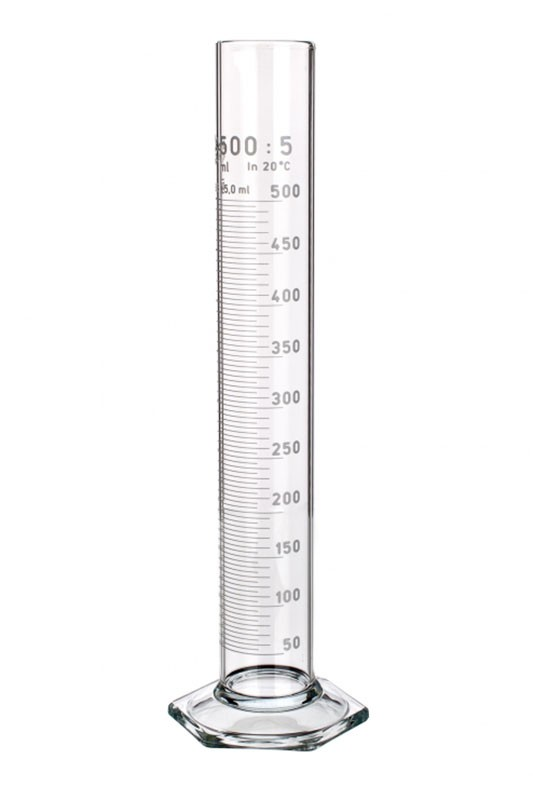
\includegraphics[scale=0.4]{obrazky/odměrný válec.jpg}
%    \end{center}
%    \caption{Odměrný válec \cite{Odměrný válec}}
%\end{figure}
%ZDROJ: https://www.vinarskepotreby.cz/odmerny-valec-1000-ml-sklo.html#gallery

\subsection{Příklad tepelné roztažnosti}
\begin{equation}
\label{objem_kapalina}
    \Delta V = \Delta V_v + \Delta V_e \left[m^3\right]
\end{equation}


\[\Delta V = 0,64 + 1,13 = 13,74 \left[ml\right]\]


\(\Delta V\) ...celkový rozdílový objem

\(\Delta V_{v}\) ...rozdílový objem vody \([m^3]\)

\(\Delta V_{e}\) ...rozdílový objem ethanolu \([m^3]\)


\begin{equation}
%\label{objem_kapalina}
    \Delta V_v = \frac{p_v}{100} \cdot V_0 \cdot \beta_v \cdot (t_1 - t_0)
\end{equation}

\[\Delta V_v = \frac{20}{100} \cdot 1 \cdot  2,14 \cdot 10^{-4} \cdot (20 - 5) = 0,64 \left[ml\right]\]

\(p_v\) ...objemový podíl vody \([\%]\) 

\(V_0\) ...počáteční objem lihoviny \([m^3]\)

\(\beta_v\) ...součinitel objemové teplotní roztažnosti vody \([\frac{m^3}{m^3 \cdot ^\circ C}]\)

\(t_1\) ...koncová teplota \([^\circ C]\)

\(t_0\) ...počáteční teplota \([^\circ C]\)

\begin{equation}
    \Delta V_e = \frac{p_e}{100} \cdot V_0 \cdot \beta_e \cdot (t_1 - t_0)\left[m^3\right] \label{objem_kapalina}
\end{equation}

\[\Delta V_e = \frac{80}{100} \cdot 1 \cdot  1,09 \cdot 10^{-3} \cdot (20 - 5) = 13,1 \left[ml\right]\]

\(p_e\) ...objemový podíl ethalonu(alkoholu) \([\%]\) 

\(\beta_e\) ...součinitel objemové teplotní roztažnosti ethalonu \([\frac{m^3}{m^3 \cdot ^\circ C}]\)




\section{Odměrné válce na alkohol}
\label{valec_na_alkohol}

%Ne příliš moc využívanou alternativou jsou válce
%Nepříliš využívaná metoda, zato mnohem efektivnější od klasického válce, kde je nutno alkohol přelévat, zde nám stačí jen láhev s alkoholem položit do středu válce a sledovat stupnici pro měřený alkohol.\\
Nepříliš využívaná metoda, zato mnohem efektivnější od klasického válce jsou odměrné válce na alkohol. Válec obsahuje několik stupnic, obvykle kolem 40, pro různé destiláty. Láhev alkoholu přiložíme k patřičné stupnici a sledujeme rysku, které odpovídá výška hladiny. Tato hodnota je rovna zbytkovému objemu v láhvi. Výhodou této metody je absence přelévání alkoholu.\\

%Lahev alkoholu přiložíme k patřičné stupnici a jaké hodnotě na stupnici od hladiny
%hodnota na stupnici, které je rovna výška hladiny je rovna zbytkovému objemu v láhvi

%Lahev alkoholu prilozime k patricne stupnici a sledujeme rysku, které odpovídá výška hladiny. Tato hodnota je rovna zbytkovému objemu v láhvi. Výhodou této metody je absence přelévání alkoholu.

\textbf{Výhody}
\begin{itemize}
    \item Cenová dostupnost\\
\end{itemize}

\textbf{Nevýhody}
\begin{itemize}
    %\item \textbf{Časově nákladné}
    \item Válec nemusí obsahovat stupnici s požadovaným alkoholem
    \item Změna tvaru láhve - Pokud výrobce alkoholu změní tvar láhve je nutné kupovat nový válec s novou stupnicí
 %(Nový alkohol - pokud v podniku přibide nový destilát k prodeji je nutné koupit válec...)
    \item Přesnost je závislá na teplotě kapaliny
    %\item Nižší přesnost měření\\\\\\\\\\\\\\\\\\
\end{itemize}

\begin{figure}[H]
    \begin{center}
        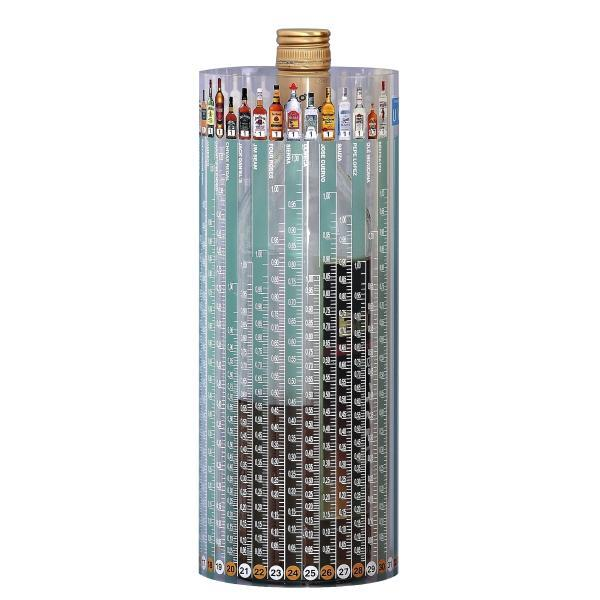
\includegraphics[scale=0.35]{obrazky/odměrný válec na alkohol.jpg}
        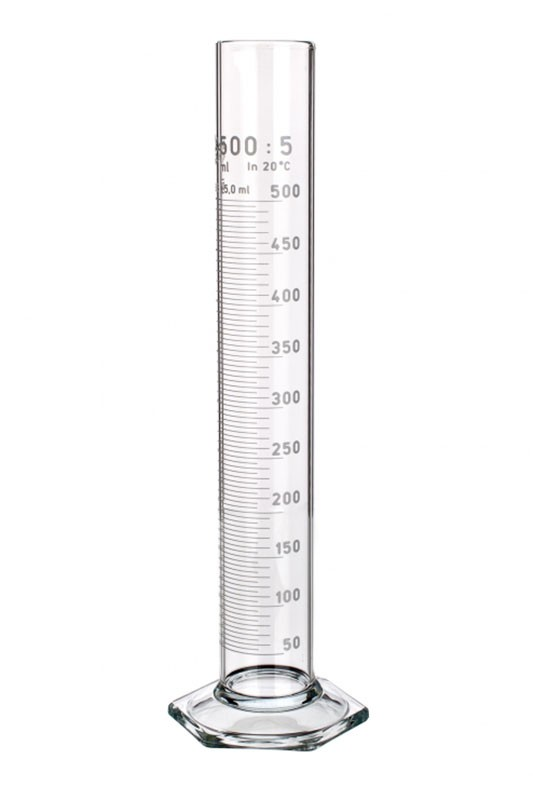
\includegraphics[scale=0.33]{obrazky/odměrný válec.jpg}
    \end{center}
    \caption{Odměrný válec na alkohol (nalevo)\cite{Odměrný válec na alkohol}, obyč. odměrný válec (napravo)\cite{Odměrný válec}}
\end{figure}
%\caption{Odměrný válec na alkohol (na levo) \cite{Odměrný válec na alkohol}}, obyč. odměrný válec (na pravo)


%%Nevyhody:
%zmena tvaru lahve - nutno kupovat nový válec s novou stupnicí
%nepresná hodnota meření

\section{Váhy}
%%foto - mozna
%%Princip přepočtu/výpočtu je podrobneji rozebrán/vice zminen v kapitole [...]

Jedná se o chytré váhy, které na základě databáze s klíčovými daty jsou schopny přepočítat hmotnost měřeného destilátu na jeho objem. 
%Tato problematika je podrobněji rozebrána v kapitole č.3.

Mezi tyto váhy spadá i navrhovaný měřicí systém, který má za úkol inovovat dosavadní měřicí metody. Jeho funkcionalita je více rozebrána v následujících kapitolách. Mezi hlavní nevýhody z pohledu uživatele patří: vysoká pořizovací cena, nutnost jednou za čas kalibrovat váhu a popřípadě doplnění stávající databáze o chybějící destiláty.
%(Databáze je zpravidla rozsáhlá a pokrývá veškeré běžně dostupné destiláty).

%...Toto není nutné pokud datábaze je rozsáhlá a pokrývá i ). více... a v případě méně známých destilátů jejich doplnění do databáze váhy.

%Existuje na světě pár společností vyvíjející váhy se stejným účelem. Bohužel jejich využití v praxi je téměř nulové z důvodu neznalosti existence těchto vah a vysoké ceny. Existuji zjednodušené řešení, kdy se využije običejná váha a aplikace pro výpočet objemu, do které se ručně zadá hmotnost destilátu.

%\section{Porovnání}
%
%Válce činí výhodné pouze jedna věc a to pořizovací cena v opačném případě se jedná o velice neefetivní způsob měření. Přes časové a finanční náklady je stále využívána, protože inventura v podnicích není laboratorní...
%
%Měření zbytkového objemu alkoholu v HoReCa podnicích není záležitostí laboratorního výzkumu tedy požadavky na přesnost jsou minimální, klíčovým fakorem je délka/doba inventury.

%\begin{equation}
%    \rho = \frac{m_{plná} - m_{prázdná}}{V_{max}} \, \left[\mathrm{kg/m^3}\right] \label{objem_kapalina}
%\end{equation}


%Výsledný vzorec pro výpočet objemu:

%\begin{equation}
%    V = \frac{m - m_{prázdná}}{\rho} \, \left[\mathrm{m^3}\right] \label{objem_kapalina}
%\end{equation}

%%%%%%%%%%%%%%%%%%%%%%%%%%%%%%%%%%%%%%%%%%%%%%%%%%%%%%%%%%%%%%
%%%%%%%%%%%%%%%%%%%%%%%%%%%%%%%%%%%%%%%%%%%%%%%%%%%%%%%%%%%%%%

%Pop

\chapter{Nově navržený systém}
%\addcontentsline{toc}{chapter}{Výpočet objemu - var. 2}
Tato kapitola popisuje obecný princip funkčnosti měřicího systému, vysvětluje přepočet hmotnosti na objem a vstupující chyby měření do systému.

\section{Postup měření}

Pro evidenci zůstatkového objemu jedné láhve je nutné naskenovat její čárový kód pomocí čtečky čárových kódů a zvážit ji. Mikrokontroler na základě získaného EAN vybere z databáze patřičná data, viz kapitola č. \ref{databaze} a přepočítá hmotnost na objem. V případě, že by čárový kód nebyl čitelný, je možné ho zadat ručně do systému prostřednictvím klávesnice. Veškeré důležité informace včetně zbytkového objemu se zobrazí na displeji.

\section{Výpočet objemu}
Hlavní komponentou vyvíjeného systému je váha, kdy z naměřené hmotnosti se vypočítá zbytkový objem pomocí vypočtené hustoty z rozdílu plné a prázdné láhve se získá hmotnost kapaliny a z údajů na etiketě se získá objem. Výhodou této metody je, že teplotní roztažnost nemá vliv na výsledek měření, protože neovlivňuje měřenou hmotnost na rozdíl od odměrných válců, kde teplotní roztažnost tvoří největší podíl chyby (přes 30 ml).

%Použijeme základní vztah pro výpočet objemu, kde hmotnost kapaliny vypočítáme jako rozdíl hmotnosti láhve se zbytkovou kapalinou a hmotnosti prázdné láhve. Výhodou této metody je, že nemá, který má u odměrných válců největší podíl chyby (přes 30 ml):

\begin{equation}
    V = \frac{m - m_{min}}{\rho} \, \left[\mathrm{m^3}\right] \label{objem_kapalina}
\end{equation}

V ...objem kapaliny

m ...hmotnost láhve se zbytkovou kapalinou \([\mathrm{kg}]\)

\(m_{min}\) ...hmotnost prázdné láhve \([\mathrm{kg}]\)

\(\rho\) ...hustota kapaliny \([\mathrm{kg/m^3}]\)
\\
\\
Výpočet hustoty kapaliny:

\begin{equation}
    \rho = \frac{m_{max} - m_{min}}{V_{max}} \, \left[\mathrm{kg/m^3}\right] 
    \label{hustota_kapalina}
\end{equation}


\(m_{max}\) ...hmotnost plné láhve \([\mathrm{kg}]\)

\(V_{max}\) ...objem plné láhve \([\mathrm{m^3}]\)
\bigskip

%Při výpočtu objemu můžeme zanedbat tepelnou roztažnost ze dvou důvodů:
%\bigskip
%\begin{enumerate}
%    \item
%    Při inventarizaci se snažíme zjistit rozdíl v množství destilátu od předchozí inventury. Běžnou praxí je využití odměrného válce, kdy objem určujeme podle rysky. Nový systém však využívá nepřímého měření založeného na hmotnosti. Kapalina při změně objemu nemění svou hmotnost, což vyvolává otázku, proč se nesoustředíme na měření zbytkové hmotnosti místo objemu. V obchodní praxi, a to i v gastronomii, se však všechny lihoviny uvádějí v jednotkách objemu. Proto je nutné naměřenou hmotnost přepočítat na objem, přičemž je klíčové, aby všechny hodnoty byly vztaženy ke stejné teplotě, aby bylo možné výsledky mezi sebou porovnávat.
%    
%    Objem se počítá pro referenční teplotu, při které byl stanoven objem plné láhve. Každý kapalný produkt (nápoje, mycí prostředky, oleje atd.) uvádí na své etiketě objem, který je obvykle vypočítán pro pokojovou teplotu 20 °C. Výhodou této metody je, že umožňuje zjistit zbytkové množství kapaliny při jakékoliv teplotě. V případě odměrných válců by bylo nutné měřit všechny destiláty při pokojové teplotě, což je časově náročné(z důvodu než se nám alkohol vytažený z lednice zahřeje na pokojovou teplotu) nebo by bylo potřeba měřit teplotu lihoviny a následně provést korekční výpočet, jaký objem by kapalina měla při pokojové teplotě. Ani jeden z těchto postupů se však běžně nepoužívá kvůli své nepraktičnosti.
%    
%    \item 
%    %Z výše uvedeného bodu vyplývá, že vypočítaný objem bude odpovídat referenční teplotě 20 °C. Stejně jako v příkladu č. [\ref{objem_kapalina}] se objeví zanedbatelná chyba, pokud bude měřicí systém stejně nebo přesnější než odměrný válec.
%    I pro případ, kdybychom nepočítali objem pro referenční teplotu, tak odchylka vyjde stejně jako v příkladu č. [\ref{objem_kapalina}], kde se objeví zanedbatelná chyba, pokud bude měřicí systém stejně nebo přesnější než odměrný válec.
%\end{enumerate}

%%%%%%%%%%%%%
%\\ 
%\\
%Velkou výhodou výpočtu objemu přes hmotnost je eliminace vlivu tepelné roztažnosti, která nemá vliv na hmotnost

%Nově navrhovaný měřicí systém je navrhovaný z důrazem na rychlost měření a i když přesnost je sekundární z důvodu hrubého odhadu, tedy zda není např. odcizena lahev. Stejně do měření objemu destilátů vstupuje hromada drobných chyb, které těžko v praxi jsme schopni ovlivnit jako je
%\begin{itemize}
%    \item Nedodržení risky na panáku - ve spěchu přelijeme
%    \item Rozlévání chlazeného alkoholu(menší objem), i když riska je dimenzovaná pro 20°C
%    \item U alkoholu s nalévačem dochází k zvětrávání a vypařování ethanolu
%    \item samotné chyby při inventůře viz kapitola výše
%\end{itemize}

\section{Chyby měření}
\label{sec:chyby měření}
Podle první kapitoly víme, že inventura je interní záležitostí podniku, pro kterou není nutné mít certifikované měřidla a přesnost si stanovuje každý zaměstnavatel sám. Bylo by tedy dobré aby nový měřicí systém měřil se stejnou nebo i lepší přesností než stávající metody, tedy odměrné válce. V praxi se nejčastěji setkáme s válci třídy B garantující přesnost $\pm$10 ml, tedy požadovaná přesnost měřícího systému je stejná nebo méně než $\pm$10 ml. V praxi by to znamenalo, že nám stačí váha s přesností $\pm$10 g, ale do systému vstupuje více chyb než jen chyba váhy.
Tedy pro určení přesnosti je nutné znát chyby které působí na měřicí systém.
\subsection{Vliv tlaku}
Vliv tlaku obecně zanedbáváme, protože má téměr nulový vliv a to i otevřených válců, kde vztlaková síla vytlačí vzduch, vytlačený vzduch pak nemá žádný vliv. Při vážení lahví jsou lahve uzavřené, tak k vytlačení vzdchu nedochází pokud nemáme na hrdle nalévátko. Dále máme tlak co působi zvnějšku lahve, tedy při vychlazené lahvi dojde k ochlazení okolního vzduchu, který způsobí 

\subsection{Vliv teploty}
\label{orosení}
I když výhodou nepřímého výpočtu objemu přes hmotnost je eliminace vlivu tepelné roztažnosti, stále se teplota může projevit ve formě orosení lahve, kde dojde ke změně její hmotnosti.

Orosení neboli kondenzace vody na těle láhve je zapříčiněno rozdílem teplot a okolní vlhkostí. Klíčový je rosný bod (RB), který lze zjistit z rovnice rosného bodu (viz vzorec č. \ref{rosný bod obecne}), kde pro 20 °C prostředí a vlhkost 50\% (běžně se pohybuje 40 - 60\%) vychází RB kolem 9,3 °C (viz příklad č. \ref{rosný bod}), což je dostačující pro vyvolání orosení u lahví chlazených na 5 °C. [z1][z2]
%FRYML, Martin. Návrh přístroje pro přímé stanovení ro
Dále na velikost orosení má vliv:
\begin{itemize}
    \item Velikost lahve - Čím větší plocha, tím více vysrážené vody.
    \item Obsah láhve - Přímo nijak neovlivňuje RB, ale tekutina uvnitř udrží déle lahev chladnou, což zapříčiní více vysrážené vody.
\end{itemize}
\smallskip
Byl tedy proveden experiment na 3 lahvích různých objemů a druhů alkoholu vychlazených na 5 °C v prostorách s teplotou 20 °C a relativní vlhkostí 53 \%. Než se naakumuluje dostatek vody na povrchu lahve chvilku to trvá, proto byla hmotnost lahve měřena po dobu 60 min. Níže tabulka č. \ref{tab:orosení} ukazuje výsledky měření, kdy nejvyšší nárust byl 0,54 g po 30 min, po této době už hmotnost lahve začala klesat na svoji původní hodnotu.

%Byl tedy proveden experiment na 3 lahvích různých objemů a obsahu kapaliny vychlazených na 5 °C v prostorách s teplotou 20 °C a relativní vlhkostí 53 \%. Než se naakumuluje dostatek vody na povrchu lahve chvilku to trvá, proto byla hmotnost lahve měřena po dobu 60 min. V praxi se zbytkový objem odměřuje krátce po vytažení lahve, tudíš je validní brat v potaz výsledky v krátkém intervalu. Níže tabulka ukazuje výsledky měření, kde po 5 min jsme byly schopni naměřit rozdíl 0,5g a nejvyšší nárus byl 1g po 45 min, po této době už hmotnost lahve klesala zpět na původní hodnotu.

\begin{table}[H]
    \centering
    \begin{tabular}{|c|c|c|c|c|}
        \hline
         Destilát & \begin{tabular}[c]{@{}c@{}}Materiál \\ lahve [g]\end{tabular} & \begin{tabular}[c]{@{}c@{}}Objem \\ lahve [l]\end{tabular} & \begin{tabular}[c]{@{}c@{}}Max. přírustek \\ hmotnosti [g]\end{tabular} & \begin{tabular}[c]{@{}c@{}} Čas max. \\ přírustku [min]\end{tabular}\\
         \hline \hline
         Nivnice borovička & sklo & 1 & 0,54 & 30\\
         \hline
         Heffron (rum) & sklo & 0,7 & 0,41 & 30\\
         \hline
         Božkov (vaječný lik.) & sklo & 0,5 & 0,17 & 20\\
         \hline
    \end{tabular}
    \caption{Přírůstky hmotnosti při orosení láhve. Měřeno s přesností na 0,01 g.}
    \label{tab:orosení}
\end{table}

V případě omezení této chyby stačí láhev před měřením otřít. Cílem ale bylo ukázat, jak vysoká chyba může nastat, pokud láhev neotřeme. Pro provozní účely je tato chyba však zanedbatelná.

%V případě měření s přesnější váhou by nám výsledné přírustky hmotnosti vykreslili xxx charakter[xx]

\subsection{Chyba hmotnosti lahve}
\label{Chyba hmotnosti lahve}
Jednou z chyb je možná odlišná hmotnost lahví při výrobě, proto bylo provedené měření rozdílu hmotností jednotlivých lahví. Pro ověření chyby z hmotnosti lahvi byla vybrána jeden z těžších destilátů. Testovných kusů bylo 15 lahví stejného typu a odlišných šarží. U stejných šarží je možné dosáhnout menší odchylky hmotnosti z důvodu identických podmínek výroby pro všechny lahve. 
Maximální rozptyl byl 3,5 g, tedy chyba \textbf{$\pm$0,85 g} (viz tab. č. \ref{tab:chyba_lahve_a_plnění}), což u měření vody je schopno zpusobit chybu o velikosti 3,5 ml. Do výpočtu za hodnotu $m_{min}$ se bude uvádět průmerná hodnota ze všech naměřených lahví.


\subsection{Chyba hmotnosti nalévače}
Některé láhve mají na svém hrdle nalévač nebo také nalévátko místo víčka, který ulehčuje rozlévání alkoholu. Jeho hmotnost se pohybuje na základě typu - lehčí nalévače jsou menší a plastové s hmotností okolo \textbf{3,8 g}, na druhé straně máme nalévače větší celokovové obsahující navíc klapku proti zvětrávání alkoholu, který váží až \textbf{50 g}. Hmotnost samotného nalévače přináší chybu do měřeného systému, proto bude kompenzovaná databázi hmotností jednotlivých nalévačů (viz kap. č. \ref{databaze}). %Dalším řešením je nalévač před měřením sundat, to ale zpomaluje vykonání inventury.

%některé obsahují klapku proti vypařování, čímž jejích hmotnost vzroste na 50 g

\begin{figure}[H]
    \begin{center}
        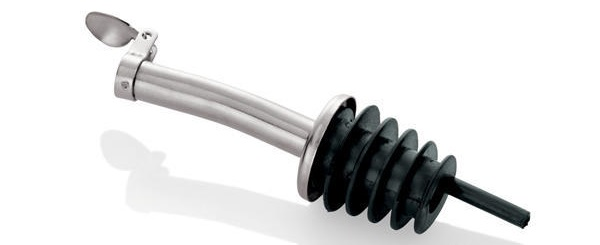
\includegraphics[scale=0.6]{obrazky/nalevac.jpg}
        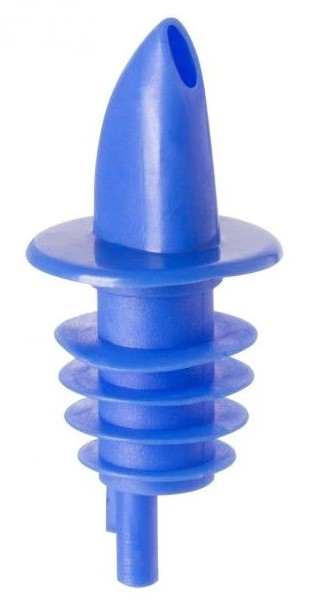
\includegraphics[scale=0.15]{obrazky/nelévač_plast.jpg}
    \end{center}
    \label{nalevačos}
    \caption{Nalévače na alkohol \cite{nalevatko}}
\end{figure}
%modré lavévátko: https://www.alkohol-shop.cz/nalevatko-plastove-modre/

\subsection{Chyba z plnění lahve}
\label{Chyby hustoty}
Pro výpočet objemu (rovnice č. \ref{objem_kapalina}) je nutná znalost hustoty destilátu, pro kterou platí předpis rovnice č. \ref{hustota_kapalina}, kde $m_{max}$ se získá navážením plné neotevřené lahve, $m_{min}$ navážením té stejné prázdné lahve, čímž se eliminuje chyba z rozptylu lahví viz kap. č. \ref{Chyba hmotnosti lahve} (chyby se navzájem odečtou) a $V_{max}$ se stanoví z etikety destilátu, který by měl odpovídat rozdílu $m_{max}$ a $m_{min}$. V této fázi vstupuje do výpočtu chyba plnění, tj. odchylka skutečného objemu od hodnoty uvedené na etiketě.

Podle nařízení EU č. 1169/2011 je v obchodních řetězcích přípustná relativní chyba objemu 1,5 \% pro kapalné produkty o objemu 500–1000 ml, což pro 1000 ml představuje toleranci $\pm$15 ml. V tomto případě by samotná chyba plnění převýšila chybu odměrných válců třídy B o objemu 1 l. Pro ověření byla provedena vlastní měření na 15 lahvích destilátu Amundsen vodka 0,5 l, kde chyba vyšla $\pm$3,65 ml (viz tab. č. \ref{tab:chyba_lahve_a_plnění}). Měřeno váhou s přesností $\pm$0,01 g a přepočteno na objem z hustoty odpovídající měřenému destilátu.


%a přepočteno na objem z hustoty odpovídající směsi vody a ethanolu v poměru 2:1 viz tabulka \ref{tab:chyba_lahve_a_plnění}. Do výpočtu samotné hustoty nám vstupuje chyba  objemu +-3,65 a chyba váhy s kterou jsou měřeny $m_{max}$ a $m_{min}$.

%---------------------------------------------------------------

%Do budoucna je v plánu databázi přesunout na server, kdesi uživatel váhy pouze stahne aktualizovanou databázi, kde je evidovaná hustota destilátu s maximální přesností pro minimalizaci chyby, ale chci dát též uživateli možnost si uložit destilát do databáze za předpokladu, že by měl exotický kousek který by nebyl uloženy v databazi na serveru a to za cenu snížení přesnosti měření tohoto destilátu. 

%Do budoucna je v plánu databázi přesunout na server, aby uživatel nemusel vést databízi a ukládat do ní nové destiláty, možnost toho ale zustane pro případ uložení destilátu, který nebude dostupný v rámci online databáze, tam budou hustoty destilátů měřeny s vyšší přesností(jednorázová investice), důvodem je jednorázová investice, která se finančně nijak nedotýka spotřebitele a navíc hlavním zdrojem chyby systému je právě ze stanovená hustoty, pro minimalizaci chyby. Přesnost váhy zůstane stejná z důvodu pořizovacích nákladů (není důvod si připlácet o několik tisíc korun za možnost naměřit objem o "3 kapky" lépe / není důvod si připlácet o několik tisíc korun za možnost naměřit objem s přesností na 0,01 ml). V případě zanedbání chyby hustoty by celková chyba systému vyšla 

%----------------------------------------------------------------


%Cílem práce je mít databázi uloženou na serveru, kde si uživatel váhy pouze stahne aktualizovanou databázi, kde je evidovaná hustota destilátu s maximální přesností pro minimalizaci chyby, ale chci dát též uživateli možnost si uložit destilát do databáze za předpokladu, že by měl exotický kousek který by nebyl uloženy v databazi na serveru a to za cenu snížení přesnosti měření tohoto destilátu. 

%Poslední možností je, pokud uživatel trvá na vysoké přesnosti a destilát neni uložen v databázi je možné si pořídit vlastní přesné zařízení pro stanovení hustoty kapaliny jako je pyknometr nebo přesná váha + přesný odměrný válec.

%Cílem zařízení je i cenově dostupná možnost pro řešení inventarizace, proto do online databáze budou ukládaná s přesností, která neovlivní výslednou přesnost zařízení. Obsluhu a správu online databáze bude provádět prodejce měřícího systému (já).

\subsection{Chyba váhy}
Posledním klíčovým faktorem je chyba váhy. Jedná se o jedinou chybu, která je ovlivnitelná, proto je nutné na základě již zmíněných chyb výše zvolit přesnost váhy takovou, aby celková přesnost systému nepřesáhla stanovenou hranici $\pm$ 10 ml.


%Teoreticky by nám stačila přesnost vyšší jak +-10g (+-10 ml vody), ale je nutné vzít v potaz i ostaní chyby, které ve výsledku mohou překročit celkovou chybu +-10 ml. Tedy přesnost váhy musí být určena z ohledem na to aby měřící systém jako celek nepřekročil celkovou chybu +-10ml.

Hmotnost se nám ve vzorcích č. \ref{objem_kapalina} a č.  \ref{hustota_kapalina} vyskytuje na 4 místech: \textit{m}, $m_{max}$ a 2x $m_{min}$. Z praktického hlediska bude měření těchto veličin prováděno stejnou váhou. Pro vypočtení přesnosti váhy je nutné znát jak se se jednotlivé chyby v systému šíří a působí na sebe, což je ukázáno na schématu obr. č. \ref{chyby} - jednotlivé proměnné jsou popsané v tab. č. \ref{tab:popis-symbolu}. (V tabulce č.x je vidět výsledná chyba systému v závislosti na různě přesných váhah běžně dostupných na trhu.) V tabulce č. \ref{tab:přesnosti vah} je vidět jak jednotlivé přesnosti běžně dostupných vah na trhu ovlivňují celkovou chybu systému. Hlavním složením destilátů je voda a ethanol, které jsou v různém poměru na základě druhu destilátu. Ethanol má menší hustotu, tedy na jednotku hmotnosti má větší objem než voda, proto byly výpočty stanoveny i pro destilát s obsahem čistého ethanolu. Výsledná přesnost systému se nachází někde mezi chybou stanovenou ethanolem a vodou. Z tabulky č. \ref{tab:přesnosti vah} odpovídá stanovenemu požadavku na přesnost do $\pm$ 10 ml, váha s přesností 0,5 g. 

V příkladu č. \ref{vypočet_objemu} je uveden výpočet pro váhu s přesností d = 0,5 g při hustotě vody. Chyba z orosení lahve nebyla ve výpočtu uvažována. V praxi je lahev vážena bezprostředně po vyjmutí z lednice, takže vysrážená voda na stěně je zanedbatelné hmotnosti (viz tab. \ref{tab:measurement_data}), navíc se dá chyba kompenzovat otřením samotné lahve. Pro stanovení přesnosti systému je využito metody maximální kumulované chyby tzv. worst-case, která uvažuje nejvyšší možné hodnoty dílčích chyb a nezohledňuje jejich pravděpodobnostní rozdělení, na rozdíl od analýzy nejistot podle GUM (Guide to the Expression of Uncertainty in Measurement).

%Na příkladu č. \ref{vypočet_objemu} je vidět konkrétní výpočet pro váhu s přesností d = 0,5 g při hustotě vody. Chyba z orosení lahve nebyla ve výpočtu uvažována. V praxi je lahev před vážením otřena a proces probíhá bezprostředně po vyjmutí z chladu, takže vysrážená voda na stěně nemá měřitelný vliv na hmotnost (viz tab. \ref{tab:measurement_data}). Pro stanovení přesnosti je využito metody chyb měření, které počítají s maximální možnou chybou tzv. "worst-case", která narozdíl on nejistot měření nepočítají s pravděpodobností výskytu chyby.

%Pro výpočet bylo využití klasických metod pro práci s chybami tzv. "worst case", kdy nam vyjde absolutní, největší možná chyba, včetně, do výpočtu jsou započítány i hrubé chyby měření, ale tím, že nám jde jen o hrubý odhad přesnosti, aby příliš "neuskočila" od přesností oměrných válců nám stačí. V případě určení přesnější chyby systému by bylo nutné zvolit stanovení chyby pomocí nejistot, které počítají s pravděpodobností výskytu chyby. Výpočet by byl složitější z důvodu nepřímého měření, který by vedl na parciální derivaci pro výpočet citlivostního koefientu a nutnosti započítat korelaci z důvodu systematických chyb způsobené opakovaným měřením stjného zařízením, výsledkem by ale byla realističtější a menší chyba systému.

%Z tabulky jde vidět, že zvyšování přesnosti váhy o 1 řád přinese zlepšení pouze o $\approx$1 ml.

\begin{figure}[H]
    \begin{center}
        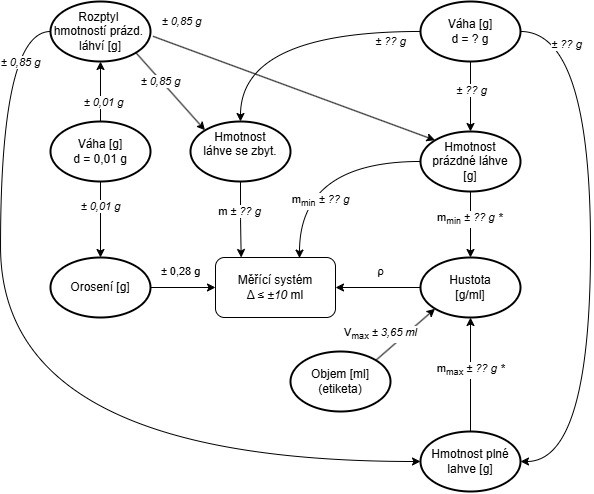
\includegraphics[scale=0.9]{obrazky/Propagace nejistot-Metoda1++.jpg}
    \end{center}
    \caption{Šíření chyb měřicím systémem}
    \label{chyby}
\end{figure}

\begin{table}[H]
    \centering
    \begin{tabular}{|l|l|}
        \hline
        \textbf{Symbol} & \textbf{Popis} \\ \hline \hline
        $m_{\text{min}}$ [g] & Hmotnost prázdné lahve \\ \hline
        $m_{\text{max}}$ [g]& Hmotnost plné lahve \\ \hline
        $m$ [g]& Hmotnost láhve se zbytkovým objemem \\ \hline
        $V_{\text{max}}$ [ml] & Max. objem lahve (etiketa) \\ \hline
        $\rho$ [g/ml]& Hustota kapaliny \\ \hline
        $\Delta_{\rho}$ [g/ml] & Chyba hustoty kapaliny \\ \hline
        $\Delta_m$ [g]& Chyba váhy pro stanovení chyby $\Delta_o$ a $\Delta_\ell$ \\ \hline
        $\Delta_o$ [g]& Chyba z orosení lahve (viz kap. č. \ref{orosení}) \\ \hline
        $\Delta$ [g]& Chyba váhy měřícího systému \\ \hline
        $\Delta_{V_{\text{max}}}$ [ml]& Chyba plnění lahve výrobcem (viz kap. č. \ref{Chyby hustoty}) \\ \hline
        $\Delta_\ell$ [g]& Chyba z rozptylu hmotnosti lahví (viz kap. č. \ref{Chyba hmotnosti lahve}) \\ \hline
        $\Delta_V$ [ml]& Chyba měřicího systému \\ \hline
    \end{tabular}
    %\caption{Popis symbolů ze schématu na obr. č.x a příkladu č.x }
    %\caption{Popis symbolů pro obr. č.x a příklad č.x }
    %\caption{Popis šířících se veličin a chyb měřicího systému}
    \caption{Popis šířících se veličin a chyb měřicím systémem}
    \label{tab:popis-symbolu}
\end{table}

\noindent\textbf{Výpočet hustoty destilátu} 
\smallskip
\newline
Hodnoty $m_{max}$, $m_{min}$ a $V_{max}$ jsou zvoleny, aby odpovídaly hustotě vody $\rho = 0,998$ g/ml v případě použití lahve s objemem 1 l. Hodnoty chyb jsou převzaty z výše uvedených kapitol (viz kap. č. \ref{orosení} až č. \ref{Chyby hustoty}). Souhrnný výpis použitých chyb v tomto příkladu je ukázán v tab. č. \ref{tab:chyby_rozloení}.

\begin{equation}
    \rho \;=\;
\frac{\bigl(m_{\max}+\Delta_{\ell}\bigr)\,\pm\Delta
      \;-\;\bigl(m_{\min}+\Delta_{\ell}\bigr)\,\pm\Delta}
     {V_{\max}\,\pm\Delta_V} = \frac{(m_{\max}-m_{\min})\;\pm\;2\Delta}
     {V_{\max}\,\pm\Delta_V}   
     \label{hustotaa}
\end{equation}
\bigskip
$m_{max}$ a $m_{min}$ se stanoví stejnou lahví, čímž se jejich chyby $\Delta_\ell$ navzájem vyruší.

\begin{equation}
\rho \;=\;
\underbrace{
\frac{(m_{\max}-m_{\min})}{V_{\max}}
}_{\text{nominální hodnota}}
\;\pm\;
\underbrace{
\frac{(m_{\max}-m_{\min})}{V_{\max}}
\left(
   \frac{2\,\Delta}{(m_{\max}-m_{\min})} \;+\; \frac{\Delta_{V_{\max}}}{V_{\max}}
\right)
}_{\text{maximální (worst-case) chyba}}
     \label{objem_kapalinaaa}
\end{equation}

\begin{equation}
\rho = \frac{(1198-200)}{1000}
\;\pm\;
\frac{(1198-200)}{1000}
\left(
   \frac{2 \cdot 0,5}{998} \;+\; \frac{3,65}{1000}
\right) = 0,998 \pm 0,00464 \text{ g/ml}
     \label{objem_kapalinaa}
\end{equation}

\noindent\textbf{Výpočet zbytkového objemu destilátu} 
\smallskip
\newline
Hodnota $m$ je rovna $m_{max}$ (zbytkový objem odpovídá plné lahvi) z důvodu získání nejvyšší relativní chyby, tedy i nejvyšší chyby celého měřicího systému.

\begin{equation}
V \;=\;
\frac{m \pm (\Delta + \Delta_\ell) \;-\; m_{\min} \pm (\Delta + \Delta_\ell)}
     {\rho \;\pm\; \Delta_\rho}\, = 
\frac{\,(m-m_{\min}) \;\pm\; 2(\Delta + \Delta_\ell)}
     {\rho \;\pm\; \Delta_\rho}
 \end{equation}

 \begin{equation}
V \;=\;
\underbrace{
\frac{\,(m-m_{\min})}
     {\rho} 
 }_{\text{nominální hodnota}}
 \pm
 \underbrace{
 \frac{(m-m_{\min})}{\rho}
\left(
   \frac{2\,(\Delta+\Delta_\ell)}{(m-m_{\min})} \;+\; \frac{\Delta_\rho}{\rho}
\right)
}_{\text{maximální (worst-case) chyba}}
 \end{equation}

 \begin{equation}
V \;=\;
\frac{(1198-200)}{0,998}
\pm
 \frac{(1198-200)}{0,998}
\left(
   \frac{2\,(0,5+0,85)}{(1198-200)} \;+\; \frac{0,00464}{0,998}
\right) = 1000 \pm 7,35 \text{ ml}
\label{vypočet_objemu}
 \end{equation}

% Requires: \usepackage{amsmath}
\begin{table}[h]
    \centering
    \begin{tabular}{|l|c|c|c|}
        \hline
        \textbf{Chyba} & \textbf{Hodnota} & \textbf{Příspěvek [ml]} & \textbf{Rel. Příspěvek [\%]} \\
        \hline \hline
        $\Delta V_{\text{max}}$ & $\pm 3{,}65 \, \text{ml}$ & 3{,}65 & 49,7 \\
        \hline
        $\Delta$ & $\pm 0{,}5 \, \text{g}$ & $4\Delta / \rho_{\text{voda}} = 2$ & 27,2 \\
        \hline
        $\Delta_\ell$ & $\pm 0{,}85 \, \text{g}$ & $2\Delta_\ell / \rho_{\text{voda}} = 1{,}7$ & 23,1 \\
        \hline
        $\Delta_V$ & $\pm 7{,}35 \, \text{g}$ & 7,35 & 100 \\
        \hline
    \end{tabular}
    \caption{Rozložení "worst-case“ chyb v systému – absolutní a relativní podíl}
    %\caption{Přehled chybových příspěvků a jejich relativní přispění}
    \label{tab:chyby_rozloení}
\end{table}

\begin{table}[H]
    \centering
    \begin{tabular}{|c|c|c|}
        \hline
        \begin{tabular}[c]{@{}c@{}}Přesnost \\ váhy [$\pm$ g]\end{tabular} & \begin{tabular}[c]{@{}c@{}}Přesnost systému \\ (voda) [$\pm$ ml]\end{tabular} & \begin{tabular}[c]{@{}c@{}}Přesnost systému \\ (ethanol) [$\pm$ ml]\end{tabular}\\ \hline \hline
         1 & 9,35 - 11,4 & 11.9 - 12,66\\ \hline
         0,5 & 7.35 - 9,90 & 9.32 - 10,76\\ \hline
         0,1 & 5.75 - 8,70 & 7.29 - 9,24\\ \hline
         0,01 & 5.39 - 8,43 & 6.83 - 8,89\\ \hline
    \end{tabular}
    \caption{Přesnost měřicího systému v závislosti na přesnosti váhy a měřeném médiu}
    \label{tab:přesnosti vah}
\end{table}


%za Δ dosadíme přesnosti běžně dostupných vah.
Největší podíl na celkové chybě systému má chyba $\Delta_{V_{\text{max}}}$ viz tab. č. \ref{tab:chyby_rozloení}. V případě výpočtu objemu za pomocí dat z online databáze, kde je hustota vedena přesně, by její chyba odpadla. Chyba systému by pak odpovídala předpisu č. \ref{chyba_objemu} - Opětovné vynechání chyby z orosení láhve. Navíc pokud dosadíme znovu váhu s přesností 0,5 g, tak nám nyní vyjde přesnost značně vyšší a to $\pm$1,35 ml pro vodu (viz příklad č. \ref{chyba_objemu_vyčislení}).

\begin{equation}
\Delta_V = \frac{\Delta + \Delta_\ell}{\rho_{voda}}
\label{chyba_objemu}
\end{equation}

 \begin{equation}
\Delta_V = \frac{0,5 + 0,85}{0,998} = 1,35 \text{ ml}
\label{chyba_objemu_vyčislení}
\end{equation}
----------------------------------------------------------------------------------------------------

xxxxxxxxxxxxxxxxxxxxxxxxxxxxxxxxxxxxxxxxxxxxxxxxxxxxxxxxxxxxxxxxxxxxxx

------------------------------------------------------------------------------------------------


%\begin{equation}
%    \pm m = \pm 5 \cdot 0.789 \, \left[\mathrm{g}\right] \label{objem_kapalina}
%\end{equation}



%\subsection{Stanovení přesnosti váhy na základě }
%Propagace nejistot pro měřící metodu A
%\subsection{Výpočet hustoty přes hmotnost lahve a stanovení přesnosti váhy}

%Zde dominantní chybu tvoří objem kapaliny, i když nám z měření vyšla chyba pouze +-xx ml, tak budem počítat z maximálně možnou dle normy ISOXXX.

%Výslednou chybu dokáže ovlivnit zda m\_min a m\_max budem měřit ze stejné láhve či nkoli. v případě stejné láhve se nám vykompenzuje chyba způsobená rozptylem hmotností lahví (+- 0,85g)

%I když chyba systému je zanedbatelná pro inevnturní účely v praxi bude systém připojen k online databázi, aby uživatel nemusel vést databízi a ukládat do ní nové destiláty, možnost toho ale zustane pro případ uložení destilátu, který nebude dostupný v rámci online databáze, tam budou hustoty destilátů měřeny s maximální přesností(jednorázová investice), důvodem je jednorázová investice, která se finančně nijak nedotýka spotřebitele a navíc hlavním zdrojem chyby systému je právě ze stanovená hustoty, pro minimalizaci chyby. Přesnost váhy zůstane stejná z důvodu pořizovacích nákladů (není důvod si připlácet o několik tisíc korun za možnost naměřit objem o "3 kapky" lépe / není důvod si připlácet o několik tisíc korun za možnost naměřit objem s přesností na 0,01 ml). V případě zanedbání chyby hustoty by celková chyba systému vyšla 



%\begin{figure}[H]
%    \begin{center}
%        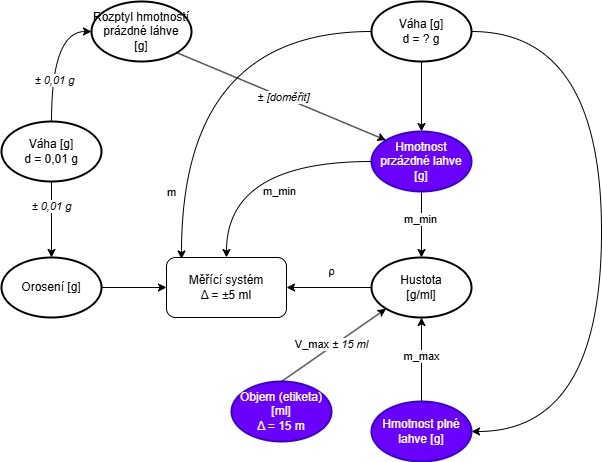
\includegraphics[scale=0.6]{obrazky/Propagace nejistot-Metoda1+.jpg}
%    \end{center}
%    \caption{Propagace nejistot - Výpočet hustoty pomocí plné láhve}
%\end{figure}
%
%//Tabulka ze vstupními parametry a jejich podílem chyby
%// nebo proste jen udělat tabulku a chyb a jejich podíl chyby


%řesnosti váhy}
%
%řednictím odměrného válce, který bude dostačující přesnosti, aby celý systém splňoval kritérium přesnosti. Přesnost válce a váhy by vůči sobě neměly být příliš rozdílný, aby měli na chybu stejný vliv (ovlivnily chybu ve stejném řádu - tedy se nejlépe navzájem vyrovnají). (pokud válec bude větší přesnosti a váha menší, přesnost válce bude automaticky kompenzována na přesnost váhy a naopak.). Dostupné válce na trhu se řídí zmíněnou normou ISOxxx. Podmínkou výběru válce je absolutní chyba pod +-5ml, tedy válce s menším objeme. Z dostupných válcu na trhu je nejvhodnějším kadinátem 250 ml válec s přesností +-1ml, kde jeho relativní chyba činí 0,4\% tedy jedná se o nejpřesnější válec na velikost vlastního objemu. Tedy pokud budem stanovovat hustotu ze vzorku pokrývající max objem válce a váhou stejné přesnosti výjde nám nejmenší relativní chyba hustoty.
%
%hustší kapa-
%kapalina bude
%vážit méně na jednotku objemu, v našem případě 10 ml. Tudíž nás zajímá, která
%složka destilátu má nejmenší hustotu. Ve své podstatě bude měřen pouze ethanol
%a voda, co se týče příměsí pro dochucení, tak ty jsou větší hustoty, proto přesnost váhy vztáhneme k ethanolu, i když nikdy nebudeme měřit 100\% ethanol, ale jeho směs s vodou a dalšími příměsi.

%Nakonec byl vytvořen Python script, který kombinuje dotupné přesnosti odměrných válců a vah. Z důvodu, jak bylo zmíněné už u válce nezáleží na absolutní chybě ale relativní, tudíž je možné využít celé spektrum dostupných válců, které se relativně jen mírně liší, díky skriptu ne že jsem schopen najít nejpřesnější kombinaci, ale vidím všechy ostatní kombinace pro přehled a jak působí na měřící systém.

%\begin{equation}
%    \pm m = \pm 5 \cdot 0.789 \, \left[\mathrm{g}\right] \label{objem_kapalina}
%\end{equation}

\begin{table}[h]
\centering
\caption{Rozpočet „worst-case“ chyb – absolutní i relativní podíl}
\renewcommand{\arraystretch}{1.15}
\begin{tabular}{@{}lcccc@{}}
\toprule
\textbf{Zdroj} & \textbf{Hodnota} & \textbf{Koef.} & \textbf{Příspěvek [ml]} & \textbf{Rel. podíl [\%]}\\
\midrule
Chyba plnění při~kalib.        & $\pm3{,}35\ \mathrm{ml}$ & $2$ & $6{,}70$ & $67{,}7$\\
Chyba váhy (\(\Delta\))        & $\pm0{,}50\ \mathrm{g}$ & $3S$ & $1{,}50$ & $15{,}2$\\
Rozptyl prázdných lahví (\(\Delta_\ell\))
                               & $\pm0{,}85\ \mathrm{g}$ & $2S$ & $1{,}70$ & $17{,}1$\\
\midrule
\multicolumn{3}{r}{\textbf{Celkem}} &
\(\boxed{\Delta V_{\text{max}} = 9{,}90\ \mathrm{ml}}\) & $100$\\
\bottomrule
\end{tabular}
\label{tab:worst_case_budget_rel}
\end{table}


\begin{table}[h]
\centering
\caption{Dosazené hodnoty a jejich příspěvek do maximální chyby objemu}
\renewcommand{\arraystretch}{1.2}
\begin{tabular}{@{}lccccc@{}}
\toprule
\textbf{Symbol} & \textbf{Popis} & \textbf{Hodnota} & \textbf{Příspěvek}\\
\midrule
$V_{\max}$      & jmenovitý objem lahve           & $1000\ \text{ml}$  & – \\
$m_{\max}$      & hmotnost plné lahve (kalibr.)   & $1180\ \text{g}$   & – \\
$m_{\min}$      & hmotnost prázdné lahve (kalibr.)& $180\ \text{g}$    & – \\
$S=\dfrac{V_{\max}}{m_{\max}-m_{\min}}$
                & převod $\,\bigl[\text{g}\rightarrow\text{ml}\bigr]$
                                                   & $1,000\ \text{ml·g}^{-1}$ & – \\[4pt]
\(\Delta V_{\text{plnění}}\)
                & chyba plnění při kalibraci      & $\pm3,35\ \text{ml}$ &
\(2\,\Delta V_{\text{plnění}} = 6,70\ \text{ml}\) \\

\(\Delta\)      & chyba váhy (každé vážení)       & $\pm0,50\ \text{g}$ &
\(3\,\Delta\,S = 1,50\ \text{ml}\) \\

\(\Delta_{\ell}\)
                & rozptyl hmotností lahví         & $\pm0,85\ \text{g}$ &
\(2\,\Delta_{\ell}\,S = 1,70\ \text{ml}\) \\
\midrule
\multicolumn{3}{r}{\textbf{Celková maximální chyba}} &
\(\boxed{\Delta V_{\text{max}} = 9,90\ \text{ml}}\) \\
\bottomrule
\end{tabular}
\label{tab:worst_case_budget}
\end{table}


\[
\Delta\rho_{\max}= \rho_{\mathrm{DB}}
\left(
   \frac{2\Delta}{m_{\max}-m_{\min}}
  +\frac{\Delta V_{\max}}{V_{\max}}
\right)
\]

\[
\Delta V_{\max}= 2\,\Delta V_{\max}^{\text{plnění}}
               +\frac{3\Delta\,V_{\max}}{m_{\max}-m_{\min}}
\tag{A}
\]


\[
\Delta V_{\max}
  = 2\,\Delta V_{\max}^{\text{plnění}}
  + \frac{(3\Delta + 2\Delta_{\ell})\,V_{\max}}
         {m_{\max}-m_{\min}}
\tag{B}
\]


\begin{equation}
    \rho \;=\;
\frac{\bigl(m_{\max}+\Delta_{\ell}\bigr)\,\pm\Delta
      \;-\;\bigl(m_{\min}+\Delta_{\ell}\bigr)\,\pm\Delta}
     {V_{\max}\,\pm\Delta_V} = \frac{(m_{\max}-m_{\min})\;\pm\;2\Delta}
     {V_{\max}\,\pm\Delta_V}   
     \label{hustotdda}
\end{equation}



\begin{equation}
\rho \;=\;
\underbrace{
\frac{(m_{\max}-m_{\min})}{V_{\max}}
}_{\text{nominální hodnota}}
\;\pm\;
\underbrace{
\frac{(m_{\max}-m_{\min})}{V_{\max}}
\left(
   \frac{2\,\Delta}{(m_{\max}-m_{\min})} \;+\; \frac{\Delta_{V_{\max}}}{V_{\max}}
\right)
}_{\text{maximální (worst-case) chyba}}
     \label{objem_kapasdalina}
\end{equation}

\begin{equation}
\rho = \frac{998}{1000}
\;\pm\;
\frac{998}{1000}
\left(
   \frac{2 \cdot 0,5}{998} \;+\; \frac{3,65}{1000}
\right) = 0,998 \pm 0,00464 ml/g
     \label{objem_kapasdalina}
\end{equation}

\begin{equation}
V \;=\;
\frac{m \pm (\Delta + \Delta_\ell) \;-\; m_{\min} \pm (\Delta + \Delta_\ell)}
     {\rho \;\pm\; \Delta_\rho}\, = 
\frac{\,(m-m_{\min}) \;\pm\; 2(\Delta + \Delta_\ell)}
     {\rho \;\pm\; \Delta_\rho}
 \end{equation}

 \begin{equation}
V \;=\;
\underbrace{
\frac{\,(m-m_{\min})}
     {\rho} 
 }_{\text{nominální hodnota}}
 \pm
 \underbrace{
 \frac{(m-m_{\min})}{\rho}
\left(
   \frac{2\,(\Delta+\Delta_\ell)}{(m-m_{\min})} \;+\; \frac{\Delta_\rho}{\rho}
\right)
}_{\text{maximální (worst-case) chyba}}
 \end{equation}

 \begin{equation}
V \;=\;
\frac{(1198-200)}{0,998}
\pm
 \frac{(1198-200)}{0,998}
\left(
   \frac{2\,(0,5+0,85)}{(1198-200)} \;+\; \frac{0,00464}{0,998}
\right) = 1000 \pm 7,35 ml
 \end{equation}



%\begin{table}[h]
%\centering
%  \begin{tabular}{c c c c}
%    \toprule
%    \textbf{Popis} &
%    \textbf{Symbol} &
%    \textbf{Hodnota} &
%    \textbf{Příspěvek {[}ml{]}} &
%    \textbf{rel. příspěvek {[}\%{]}} \\ \midrule
%    Hmotnost prázdné láhve              & $m_{\min}$ & $180\;\text{g}$          & --      & --   \\
%    Hmotnost plné láhve                 & $m_{\max}$ & $1180\;\text{g}$         & --      & --   \\
%    Hmotnost láhve se zbytkovým objemem & $m$        & $m = m_{\max}$           & --      & --   \\
%    Max. objem láhve (etiketa)          & $V_{\max}$ & $1000\;\text{ml}$        & --      & --   \\
%    Hustota kapaliny (voda)             & $\rho$     & $1000\;\text{g\,ml}^{-1}$& --      & --   \\
%    Chyba hustoty kapaliny              & $\Delta\rho$ & --                     & --      & --   \\[2pt]
%    Chyba váhy pro stanovení $\Delta_o,\,\Delta_\ell$ & $\Delta_m$ & $\pm 0{,}01\;\text{g}$ & -- & -- \\[2pt]
%    Chyba z orosení láhve (včetně $\Delta_m$) & $\Delta_o$ & $\pm 0{,}28\;\text{g}$ & -- & -- \\[4pt]
%    Chyba váhy měřicího systému         & $\Delta$   & $\pm 3{,}35\;\text{ml}$  & $(4\Delta)/\rho = 2,00$ & 27,2 \\
%    Chyba plnění láhve výrobcem         & $\Delta V_{\max}$ & $\pm 3{,}65\;\text{ml}$ & $\Delta_m = 3,65$ & 49,7 \\
%    Chyba z rozptylu hmotnosti láhví \newline (včetně $\Delta_m$) & $\Delta_\ell$ & $\pm 0{,}85\;\text{g}$ & $2\Delta_\ell/\rho = 1,70$ & 23,1 \\[4pt]
%    \textbf{Chyba měřicího systému}     & $\Delta V$ & -- & \textbf{7,35} & \textbf{100} \\ \bottomrule
%  \end{tabular}
%  \caption{Rekapitulace složek worst-case chyby měřicího systému.}
%\end{table}

% Requires: \usepackage{array}

%\begin{table}[h]
%    \centering
%    \begin{tabular}{|>{\raggedright}p{4cm}|c|c|c|c|}
%    \hline
%    \textbf{Popis} & \textbf{Symbol} & \textbf{Hodnota} & \textbf{Příspěvek [ml]} & \textbf{rel. Příspěvek [\%]} \\ \hline
%    Hmotnost prázdné láhve & $m_\text{min}$ & 180 g & - & - \\ \hline
%    Hmotnost plné láhve & $m_\text{max}$ & 1180 g & - & - \\ \hline
%    Hmotnost láhve se zbytk. Objemem & $m = m_\text{max}$ & - & - & - \\ \hline
%    Max. objem láhve (etiketa) & $V_\text{max}$ & 1000 ml & - & - \\ \hline
%    Hustota kapaliny (voda) & $\rho$ & 1000 g/ml & - & - \\ \hline
%    \textbf{Chyba hustoty kapaliny} & $\Delta_{\rho}$ & & & \\ \hline
%    Chyba váhy pro stanovení $\Delta_m$ a $\Delta_{\rho}$ & $\Delta_m$ & $\pm0,01$ g & & \\ \hline
%    Chyba z orosení láhve (viz kap. č.) & & & & \\ \hline
%    včetně chyby váhy $\Delta_m$ & $\pm$ & $3,35$ ml & & \\ \hline
%    Chyba váhy měřicího systému & $\Delta$ & & & \\ \hline
%    včetně chyby váhy $\Delta_m$ & $\pm 0,28$ g & $\frac{44}{\rho^2} =$ & $27,2$ \\ \hline
%    Chyba plnění láhve výrobcem (viz kap. č. x) & $\Delta V_\text{max}$ & $\pm3,65$ ml & & \\ \hline
%    včetně chyby váhy $\Delta_m$ & & & $49,7$ \\ \hline
%    Chyba z rozptylu hmotnosti láhví (viz kap. č. x) & & & & \\ \hline
%    včetně chyby váhy $\Delta_m$ & $\pm0,85$ g & $\pm1,97$ & $23,1$ \\ \hline
%    \textbf{Chyba měřicího systému} & $\Delta V$ & & $7,35$ & $100$ \\ \hline
%    \end{tabular}
%    \caption{Tabulka chyb a příspěvků měření}
%    \label{tab:chyby-prispevky}
%\end{table}

%%%%%%%%%%%%%%%%%%%%%%%%%%%%%%%%%%%%%%%%%%%%%%%%%%%

%\[
%\rho \;=\;
%\frac{\bigl(m_{\max}+\Delta_{\ell}\bigr)\,\pm\Delta
%      \;-\;\bigl(m_{\min}+\Delta_{\ell}\bigr)\,\pm\Delta}
%     {V_{\max}\,\pm\Delta_V} = \frac{(m_{\max}-m_{\min})\;\pm\;2\Delta}
%     {V_{\max}\,\pm\Delta_V}   
%\]
%
%\(m_{min}\) ...hmotnost prázdné láhve \([\mathrm{g}]\)
%
%\(m_{max}\) ...hmotnost plné láhve \([\mathrm{g}]\)
%
%\(\rho\) ...hustota kapaliny \([\mathrm{g/ml}]\)
%
%\(\Delta\) ...chyba váhy \([\mathrm{g}]\)
%
%\(\Delta_\ell\) ...chyba z rozptylu hmotnosti prázdných láhví \([\mathrm{g}]\)
%
%\(\Delta_V\) ...chyba objemu plné láhve (etiketa) \([\mathrm{g}]\)
%
%\[
%m_{\rho} \;=\; m_{\max} \;-\; m_{\min}
%\]
%
%\(m_{\rho}\) ...hmotnost kapaliny pro stanovení hustoty\([\mathrm{g}]\)
%
%\[
%\rho \;=\;
%\frac{m_{\rho} \,\pm\, 2\Delta}
%     {V_{\max} \,\pm\, \Delta_{V_{\max}}} = \frac{m_{\rho}}{V_{\max}}
%\;\pm\;
%\frac{m_{\rho}}{V_{\max}}
%\left(
%   \frac{2\,\Delta}{m_{\rho}} \;+\; \frac{\Delta_{V_{\max}}}{V_{\max}}
%\right)
%\]


%\[
%V \;=\;
%\frac{%
%      m \,\pm\, (\Delta + \Delta_\ell)
%      \;-\;
%      m_{\min} \,\pm\, (\Delta + \Delta_\ell)
%     }{%
%      \rho \,\pm\, \Delta_\rho
%     }.
%\]
%
%V ...objem kapaliny
%
%m ...hmotnost láhve se zbytkovou kapalinou \([\mathrm{kg}]\)
%
%\(\Delta_\rho\) ...chyba hustoty \([\mathrm{g/ml}]\)
%
%\[
%m_{\mathrm{zb}} \;=\; m \;-\; m_{\min}\,.
%\]
%
%\(m_{zb}\) ...hmotnost zbytkové kapaliny v láhvi \([\mathrm{g}]\)
%
%\[
%V \;=\;
%\frac{\,m_{\mathrm{zb}} \;\pm\; 2(\Delta + \Delta_\ell)}
%     {\rho \;\pm\; \Delta_\rho}\,.
%\]
%
%\begin{center}    
%\boxed{%
%V \;=\;
%\frac{%
%      \bigl[m - m_{\min}\bigr]
%      \,\pm\, 2\bigl(\Delta + \Delta_{\ell}\bigr)}%
%     {%
%      \dfrac{m_{\max}-m_{\min}}{V_{\max}}
%      \,\pm\,
%      \dfrac{m_{\max}-m_{\min}}{V_{\max}}
%      \!\left(
%        \dfrac{2\Delta}{m_{\max}-m_{\min}}
%        +\dfrac{\Delta_{V_{\max}}}{V_{\max}}
%      \right)}%
%}\tag{V\text{-full}}
%\end{center}
%
%\begin{center}  
%\boxed{
%V \;=\;
%\frac{%
%      V_{\max}
%      \bigl[m - m_{\min} \,\pm\, 2(\Delta + \Delta_{\ell})\bigr]}%
%     {%
%      (m_{\max}-m_{\min})
%      \left[
%        1
%        \,\pm\,
%        \left(
%          \dfrac{2\Delta}{m_{\max}-m_{\min}}
%          +\dfrac{\Delta_{V_{\max}}}{V_{\max}}
%        \right)
%      \right]}%
%\tag{V\text{-simp}}}
%\end{center}  
%
%\boxed{
%V
%=
%\underbrace{\frac{m-m_{\min}}{m_{\max}-m_{\min}}\,V_{\max}}_{\text{nominalní hodnota}}
%\;\pm\;
%\underbrace{\Bigl[
%      2\,\Delta_{V_{\text{max}}}
%      \;+\;
%      \bigl(3\,\Delta+2\,\Delta_{\ell}\bigr)\,
%      \frac{V_{\max}}{m_{\max}-m_{\min}}
%\Bigr]}_{\text{maximální (worst-case) chyba}}
%
%\tag{V\text{-simp}}}
%
%\bigskip
%Ukázka výpočtu chyby měřicího systému pro $\Delta$ = 0,5 g, $\rho$ = hustota vody = 1 g/ml (V$_{max}$ = 1 l, m\_max = 1200 g a m\_min = 200 g), $\Delta_\ell$ = 0,85 [\ref{Chyba hmotnosti lahve}], $\Delta_{V_{\text{max}}}$ = 3,65 ml [\ref{Chyby hustoty}]
%
%\[
%\Delta_V = 2\,\Delta_{V_{\text{max}}}
%      \;+\;
%      \bigl(3\,\Delta+2\,\Delta_{\ell}\bigr)\,
%      \frac{V_{\max}}{m_{\max}-m_{\min}}
%\]
%
%\[
%\Delta_V = 2 \cdot 3,65
%      \;+\;
%      (3\cdot0,5+2\cdot0,85)\,
%      \cdot\underbrace{\frac{1000}{1200-200}}_{\text{= 1 $\simeq \rho_{voda}$}}=\pm 9,90 ml
%\]
\chapter{Sériová komunikace}
\label{Sériová komunikace}
Seriová komunikace je způsob přenosu dat mezi dvěma nebo více zařízeními, při kterém se data posílají po jednotlivých bitech po jediném vodiči nebo bezdrátovém kanálu. Touto formou budou komunikovat jednotlivé komponenty navrhovaného měřicího systému, proto je vhodné si tuto terminologii/problematiku objasnit. Nejrozšířenějšími standardy a protokoly pro sériovou komunikaci jsou RS-232, UART, SPI, USB. \cite{ser kom}


%Sériová komunikace je posílání dat v řadě nebo-li bit po bitu
%Seriová komunikace je způsob přenosu dat mezi dvěma nebo více zařízeními, při kterém se data posílají po jednotlivých bitech po jediném vodiči nebo bezdrátovém kanálu. Seriová komunikace je vhodná pro dlouhé vzdálenosti a nižší rychlosti, protože vyžaduje méně vodičů než paralelní komunikace, která se běžně využívá na deskách plošných spojů. Seriová komunikace se dělí na synchronní a asynchronní, podle toho, zda je potřeba precizně synchronizovat časování při vysílání mezi vysílačem a přijímačem. Pro naše účely se budem zabývat pouze asychronní komunikací. Seriová komunikace se používá pro různé účely, jako je komunikace s modemem, tiskárnou, senzory, paměťovými kartami, síťovými adaptéry a dalšími periferiemi. Běžné a obecně známé standardy a protokoly pro seriovou komunikaci jsou RS-232, UART, SPI, USB.
%...precizně synchronizovat časování při vysílání mezi vysílačem a přijímačem (tohle poradil Pety)
%\cite{ser kom}
%[zdroj]
%zdroj kniha o seriove komunikaci
%\begin{figure}[!h]
%    \begin{center}
%        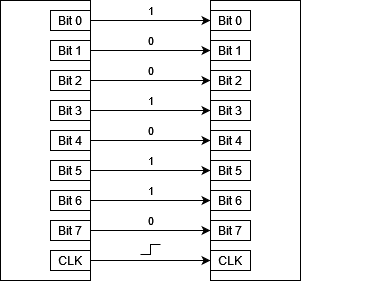
\includegraphics[scale=0.62]{obrazky/paralelni_komunikace.png}
%        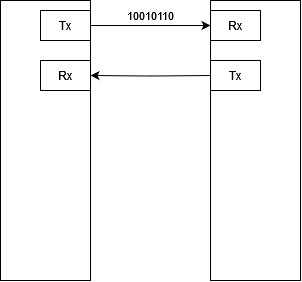
\includegraphics[scale=0.62]{obrazky/Seriova komunikace.png}
%    \end{center}
%    \caption[Porovnání seriové a paralelní komunikace]{Porovnání paralelní(vlevo) a sériové(vpravo) komunikace. Sériová komunikace v topologii pro UART protokol}
%\end{figure}
%zdroj: https://www.rohde-schwarz.com/cz/products/test-and-measurement/essentials-test-equipment/digital-oscilloscopes/understanding-serial-protocols_254522.html#gallery-5

%\section{Komunikační protokoly}
%Komunikační protokol je sada pravidel a dohod, které umožňují zařízením komunikovat mezi sebou. Protokol definuje formát, obsah, časování a řízení toku dat mezi odesílatelem a příjemcem. \cite{ser kom}

\section{komunikační protokol UART}
\label{UART protokol}
Komunikační protokol je sada pravidel a dohod, které umožňují zařízením komunikovat mezi sebou. Protokol definuje formát, obsah, časování a řízení toku dat mezi odesílatelem a příjemcem.

UART (Universal asynchronous receiver - transmitter) protokol je jeden z nejstarších a nejjednodušších komunikačních protokolů, který používá sériovou linku pro přenos dat mezi dvěma zařízeními. UART protokol nemá společný hodinový signál, ale zařízení se mezi sebou jinými prostředky dohodnou na rychlosti přenosu (baud rate) a formátu dat (počet bitů, parita, stop bit). UART protokol používá čtyři signály: TX (vysílač), RX (přijímač), GND (zem) a volitelně RTS/CTS (řízení toku). \cite{ser kom} %UART protokol je často používán pro komunikaci s periferními zařízeními, jako jsou modemy, senzory, displeje nebo klávesnice. \cite{ser kom}

\subsection{UART datový paket}
\label{UARTt}
Datový paket popisuje posloupnost neboli datový tok bitů. Z obrázku č. \ref{UART packet} je vidět, že paket je ohraničený START (logická úroveň 1) a STOP (logická úroveň 0) bitem, které udávají začátek a konec zprávy. Díky tomu jsme schopni separovat více jdoucích paketů v řadě. Za START bitem následuje datový rámec, který bývá z pravidla 8 bitový (1 Bajt) a nese informaci uživatele, ostatní bity slouží k "řízení" paketu. Dále je zde paritní bit, který aplikuje na datový rámec logickou operaci XOR. Existují dva druhy parity: sudá - XOR operace je rovna 1, pokud počet jedniček v datovém rámci je sudý.  Pro lichou paritu platí to stejné v případě, že počet jedniček v rámci je lichý. Paritní bity nejsou vždy využity. Záleží na konkrétní aplikaci. Slouží ke kontrole, jestli datový rámec není poškozen. \cite{ser kom} %[zdroj:] %https://cs.wikipedia.org/wiki/Paritn%C3%AD_bit
%*XOR je 

\begin{figure}[!h]
    \begin{center}
        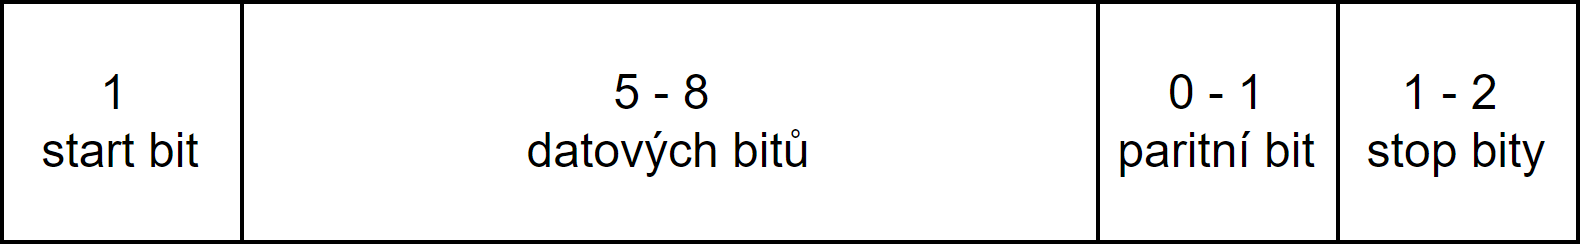
\includegraphics[scale=0.5]{obrazky/datovy ramec UART - final.png}
    \end{center}
    \caption{Datový tok protokolu UART}
    \label{UART packet}
\end{figure}
%ZDROJ: https://yarkov.tech/en/blog/2022-11-04/using-the-web-serial-api-to-communicate-with-the-microcontroller/

\section{Komunikační standard RS-232}
Komunikační standard je soubor pravidel a specifikací, které definují, jak mají zařízení komunikovat mezi sebou. Komunikační standard zahrnuje fyzické, elektrické, funkční a mechanické charakteristiky komunikačního rozhraní. Například RS-232 je komunikační standard pro sériovou komunikaci mezi počítačem a modemem.
RS-232 definuje:
\begin{itemize}
    \item \textbf{Elektrické charakteristiky:} RS-232 používá napěťové úrovně od -15 V do +15 V pro reprezentaci logických stavů 0 a 1. RS-232 také specifikuje maximální rychlost přenosu, impedanci, toleranci zkratu a další parametry signálu.
    \item \textbf{Funkční charakteristiky:} RS-232 popisuje funkce a smysl definovaných signálů, které se používají pro řízení toku dat mezi zařízeními. Některé z těchto signálů jsou například: TXD (odesílaná data), RXD (přijímaná data), RTS (požadavek na odeslání), CTS (povolení k odeslání) a DTR (zařízení a terminál je připraveno navázat spojení). %DTR(zařízení připraveno)
    \item \textbf{Mechanické charakteristiky:} RS-232 definuje také fyzický tvar a rozmístění pinů konektorů, které se používají pro propojení zařízení. Nejběžnějšími typy konektorů jsou DB9 a DB25, které mají devět a pětadvacet pinů, viz obrázek č.\ref{rs232_obr} \cite{ser kom}
\end{itemize}
%Zdroj dokument o seri. komunikaci

\begin{figure}[!h]
    \begin{center}
        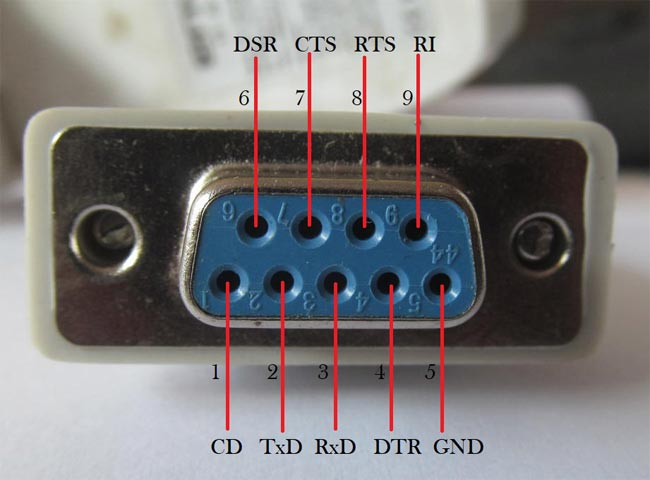
\includegraphics[scale=0.4]{obrazky/RS232.jpeg}
    \end{center}
    \caption{Konektor DB9 s popisem pinů. \cite{RS232}}
    \label{rs232_obr}
\end{figure}
%zdroj RS-232: https://www.pbxdom.com/blog/engineering/what-is-serial-rs232-port-interface/

%\section{USB}
%Universal Serial Bus zkráceně USB je průmyslový standard, který stanovuje specifikace pro kabely a konektory na zařízeních, stéjně jako výše zmíněné RS-232.
%
%USB diponuje konektory Vcc (napájení 5V), datovými piny D+ (vysílač), D- (přijímač) a GND(zem). Obsahuje další konektory jako superrychlostní datové piny, ale těmi se zabívat nebudeme.
%
%Existuje několik verzí USB, které se od sebe líší jak fyzickými rozměry(tvarem konektoru) tak i přenosovou rychlostí. My se budem zabívat verzí USB 2.0 a 3.x s konektorem typu A
%
%USB přišlo jako "náhrada" za starší standard RS-232. USB je rozměrově menší a několika násobně rychlejší.[zdroj]
%%zdroj ai, citoval wikinu
%
%%asi vymazat tuhle sračku
%\begin{figure}[!h]
%    \begin{center}
%        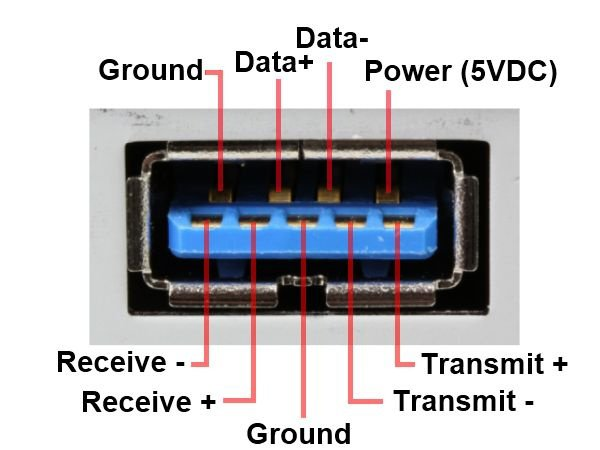
\includegraphics[scale=0.4]{obrazky/USB.jpg}
%    \end{center}
%    \caption{USB 3.1/3.2 A s popisem pinů}
%\end{figure}
%%zdroj USB: https://www.quora.com/If-USB-3-0-type-A-support-max-output-at-5v-0-9a-why-are-there-so-many-type-A-to-type-C-cables-that-supposedly-support-5v-3a
%%Doporuceno zmenit zdroj
\chapter{Nově navržený systém}
\label{Nově navržený systém}
%V této kapitole se budem zabívat nově navrženým systémem, jejíma komponentama a... 
Nově navržený systém se skládá z databáze a 5 hlavních komponent navzájem propojených: modul s výpočetní jednotkou, váha, čtečka čárového kódu a dotykový displej. Dále je možnost připojit systém k počítači pro správu databáze. 

\section{Postup měření}%/Princip/funkcionalita
Pro evidenci zůstatkového objemu jedné láhve je nutné naskenovat její čárový kód pomocí čtečky čárových kódů a zvážit ji. Modul s výpočetní jednotkou na základě získaného EAN vybere z databáze patřičná data, viz kapitola č. \ref{databaze} a přepočítá hmotnost na objem. V případě, že by čárový kód nebyl čitelný, je možné ho zadat ručně do systému prostřednictvím klávesnice. Veškeré důležité informace včetně zbytkového objemu se zobrazí na displeji. %Pro výpis všech naměřených dat je možné systém připojit k počítači a nechat si je vytisknout do formátu .xlsx pomocí navržené desktopové aplikace. Tato aplikace slouží i ke správě databáze.
%Do budoucna k měřicimu systému bude vyvíjena desktopová aplikace běžící na stolním počítačí/notebooku. Mikrokontroler bude k počítači připojen prostřednictvím USB portu
%Do budoucna pro výpis všech naměřených dat bude možné systém připojit k počítači a nechat si je vytisknout do formátu  .xlsx pomocí navržené desktopové aplikace. Tato aplikace slouží i ke správě databáze.

Do budoucna bude vyvíjena desktopová aplikace pro editaci databáze[č.5.3] a zpracování naměřených dat, jako je například tisk do formátu .xlsl. Měřicí systém bude propojený s počítačem skrz USB kabel nebo Wi-Fi.

\section{Blokové schéma}
%FOTO
%Výpočetní jednotka Raspberry pi pracuje s databázi dat jednotlivých destilátů. V první řadě je nutné tuhle databází vytvořit a implementovat prostřednictvím desktopové aplikace. 
\begin{figure}[!h]
    \begin{center}
        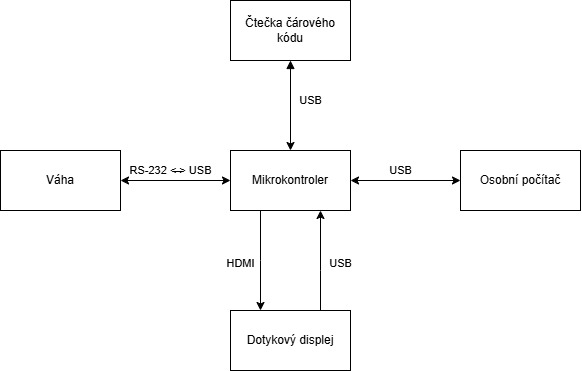
\includegraphics[scale=0.7]{obrazky/Blokové schéma.jpg}
    \end{center}
    \caption{Blokové schéma nově navrženého systému}
    \label{blokove_schema}
\end{figure}

\section{Databáze}
\label{databaze}
%Celý systém je závislý na datech, které nesou informace o názvu destilátu
Aby bylo možné přepočítat hmotnost na objem je nutné znát předem hmotnost prázdné a plné láhve a její maximální objem. Postup výpočtu je zmíněn v kapitole č. \ref{odkazos}. Tyto data jsou uloženy v relační\footnote{Data uložený v tabulkách, kde sloupce reprezentují atributy a řádky jednotlivé záznamy, řádky jsou propojeny pomocí tzv. klíčů. Tabulky \ref{databaze_destilatu} a \ref{tab:my_label} mají prohozené řádky a sloupce z důvodu lepšího umístění na stránku.} databázi včetně informací jako jsou: název destilátu, EAN kód, maximální objem, nebo adresa k obrázku daného produktu.
%K datům se přistupuje pomocí EAN kódu nebo názvem destilátu zadaný klávesnicí.

%Některé destiláty, mají na svém hrdle nalévač místo vršku, který mění hmotnost láhve. Aby naš systém byl časově efektivní, tak implementujeme druhou databázi 

%Některé destiláty mají na svém hrdle nalévátko (obrázek č. \ref{nalevačos}) místo víčka, který mění hmotnost láhve. V takovém případě bychom museli nalévač nahradit víčkem, aby hmotnost láhve odpovídala předpisu funkce, což je časově neefektivní. Místo toho byla navržena druhá databáze, obsahující hmotnosti různých nalévačů. Vzorec pro výpočet objemu ve výchozím nastavení počítá s víčkem na láhvi, proto uživatel musí při měření zakliknout pomocí klávesnice, že chce měřit objem s nalévačem. Při výpočtu dojde k nahrazení hmotnosti víčka hmotností nalévače a následně dojde k výpočtu výsledného objemu.

Některé destiláty mají na svém hrdle nalévač nebo také nalévátko (obrázek č. \ref{nalevačos}) místo víčka, který mění hmotnost láhve. V takovém případě bychom museli nalévač nahradit víčkem, aby hmotnost láhve odpovídala předpisu rovnice č.xyz (skutečná hmotnost prázdné láhve musí odpovídat s hodnotou hmotnosti prázdné láhve v databázi), což je časově neefektivní. Místo toho byla navržena druhá databáze, obsahující hmotnosti různých nalévačů. Vzorec pro výpočet objemu ve výchozím nastavení počítá s víčkem na láhvi, proto uživatel musí při měření zakliknout v aplikaci, že chce měřit objem s nalévačem. Při výpočtu dojde k nahrazení hmotnosti víčka hmotností nalévače a následně dojde k výpočtu výsledného objemu.


%Vyhledání destilátu a jeho dat je porstřednictvím EAN kódu nebo jeho názvu.

Obě databáze jsou uložené v mikrokontroléru.

%FOTO
\begin{table}[H]
\centering
\begin{tabular}{|l|l|l|l|}
\hline
 & Destilát č. 1   & Destilát č. 2   &  . . . \\ \hline
\textbf{Název destilátu} [-] [\textit{TEXT}] &   &    &  \\ \hline
\textbf{EAN kód} [-] [\textit{INTEGER}]&  &    &        \\ \hline
\textbf{Hmotnost prázdné láhve} [g] [\textit{numeric}] &    &  &        \\ \hline
\textbf{Hmotnost plné láhve} [g] [\textit{numeric}] &    &    &  \\ \hline
\textbf{Hmotnost víčka} [g] [\textit{numeric}] &    &    &  \\ \hline
\textbf{Maximální objem láhve} [l] [\textit{numeric}] &    &    &  \\ \hline
\textbf{Množství alkoholu} [\%] [\textit{numeric}] &    &    &  \\ \hline
\textbf{Adresa obrázku} [-] [\textit{TEXT}] &    &    &  \\ \hline
%Obrázek: obsahuje adresu/název obrázku, který je uložen ve složce
\end{tabular}
\label{databaze_destilatu}
\caption{Databáze destilátů}
\end{table}


\begin{table} [H]
    \centering
    \begin{tabular}{|l|l|l|l|}
    \hline
         & Nalévač č. 1 & Nalévač č. 2 &  . . .\\ \hline
         \textbf{Název nalévače} [-] [\textit{TEXT}] & & &\\ \hline
         \textbf{Výrobce} [-] [\textit{TEXT}] & & &\\ \hline
         \textbf{Hmotnost} [g] [\textit{numeric}] & & &\\ \hline
         \textbf{Adresa obrázku} [-] [\textit{TEXT}] & & &\\ \hline
    \end{tabular}
    \caption{Databáze nalévačů}
    \label{tab:my_label}
\end{table}

%\begin{figure}[!h]
%    \begin{center}
%        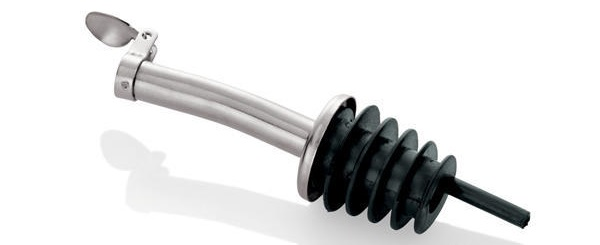
\includegraphics[scale=0.6]{obrazky/nalevac.jpg}
%    \end{center}
%    \label{nalevačos}
%    \caption{Nalévač na alkohol \cite{nalevatko}}
%\end{figure}
% \definecolor{Silver}{rgb}{0.752,0.752,0.752}
% \begin{table}[!h]
%     \centering
%     \begin{tabular}
%         {
%         cell{1}{4} = {c},
%         hlines = {Silver},
%         vlines = {Silver},
%         }
%         Název & hmotnost\\
%         Nalévač č.1 & x\\
%     \end{tabular}
%     \caption{Caption}
%     \label{tab:my_label}
% \end{table}
%\usepackage{color}
%\usepackage{tabularray}
%\definecolor{Silver}{rgb}{0.752,0.752,0.752}
%\begin{tabular}[
%  label = none,
%  entry = none,
%]{
%  cell{1}{4} = {c},
%  hlines = {Silver},
%  vlines = {Silver},
%}
%Název destilátu & destilát č.1 & destilát č.2 & . . . \\
%EAN kód & & & \\
%hmotnost prázdné láhve & & & \\
%hmotnost plné láhve    &              & & \\
%hmotnost víčka         &              &              &       \\
%obrázek                &              &              &       \\
%max. objem             &              &              &       
%\end{tabular}
%Tabulka destilátů
%Nazev | EAN | k | q | m_víčko | max_objem | obrazek | poznamka
%Tabulka druhů nalévačů
%Nazev | m_nalevač | obrazek

\section{Váha}

Nejdůležitější komponentou systému je váha pro výpočet zbytkového objemu z naměřené hmotnosti láhve, viz kapitola č.\ref{Přepočet hmotnosti na objem}.  Proto v této podkapitole rozeberu požadavky, výběr váhy a její alternativy.
%
%Váhy jsou zařízení, která slouží k měření hmotnosti objektů. Existuje mnoho typů vah, ale základní princip je stejný. Váhy se skládají ze dvou hlavních částí: měřicího mechanismu a zobrazovacího mechanismu.
%
%Měřicí mechanismus se skládá z vážícího tělesa a pružiny. Když položíte objekt na váhu, pružina se stlačí a vážící těleso se posune dolů. Tento pohyb se přenáší na měřicí stupnici, která ukazuje hmotnost objektu.
%
%Zobrazovací mechanismus se skládá z displeje a elektronického obvodu. Elektronický obvod přijímá signál od měřicího mechanismu a převádí ho na čitelný formát pro displej. Displej pak zobrazuje hmotnost objektu.[zdroj]
%
%\subsection{Elektronická část váhy}
%
%Elektronická část váhy se skládá z senzoru a elektronického obvodu. Senzor měří deformaci, kterou způsobuje vážený objekt, a převádí ji na elektrický signál. Tento signál je poté zpracován elektronickým obvodem, který obsahuje A/D převodník a mikroprocesor.
%
%Senzory používané v elektronických vahách jsou obvykle tenzometry nebo load cells. Tenzometry jsou malé senzory, které měří změnu odporu, když jsou deformovány. Load cells jsou senzory, které měří změnu napětí, když jsou deformovány. Oba typy senzorů jsou velmi přesné a umožňují měření hmotnosti s vysokou přesností.
%
%A/D převodník převádí analogový signál z senzoru na digitální signál, který může být zpracován mikroprocesorem. Mikroprocesor pak zpracovává signál a zobrazuje výslednou hmotnost na displeji. [zdroj]
%
\subsection{Požadavky na váhu}

%Dle výpočtů[], aby systém splnil toleranci +-5ml je nutné volit váhu s přesností menší jak 0,075g, tomu z dostupných vah na trhu odpovídá váha s přeností 0,01g, kde výsledná přesnost měřícího systému pro metodu x je pod limitem přesnosti válce třídy A a nebo přesnost 0,1g, kde jsem na hraně.
%Další možností jak 

%bude pro metodu č. x XY+-ml a pro metodu a nebo o něco méně přesná 0,1 g, kde výsledná přesnost vychází +-5,2 ml

%Z komerčních důvodů byla vybrána váha s přesností 0,5g, kde přesnost celého systému 

%Tabulka: metoda(A,B,C), přesnost váhy(C=2váhy), přesnost systému, cena

Hlavním požadavkem je oboustranný otevřený komunikační port pro čtení dat a odesílání požadavku na jejich zaslání prostřednictvím sériové linky do řídicí jednotky, je tedy nutné znát přesný popis přenosu dat. Tyto požadavky zpravidla splňují laboratorní a průmyslové váhy, kde se očekává, že data budou zpracovávána pomocí aplikačního softwaru.

Váživost (maximální hmotnost, která lze na váze navážit) se požaduje minimálně 2 kg. Hmotnost prázdné láhve u většiny destilátů se pohybuje od 500 do 800 g a samotný obsah láhve je od 500 do 1000 ml, tudíž až necelý 1 kg. V případě robustnějších lahví okolo 1 kg by váživost do 2 kg nemusela stačit, proto je vhodnější volit 3 kg. Větší váživost jak 3 kg, by neměla pro běžné podniky HoReCa význam, navíc s vyšší váživostí úměrně klesá její přesnost a roste cena váhy.

Přesnost, jinak řečeno rozlišení nebo odčitatelnost, se udává v dílcích(d). Dílek je nejmenší hodnota hmotnosti, kterou lze z displeje váhy odečíst.\cite{vazivost} Měření zbytkového objemu destilátu při inventurách není záležitostí "laboratorního měření" a zákon nestanovuje s jakou přesností je nutné měřit objem v láhvích pro inventurní účely. Obecně na 
přesnost není kladen velký důraz. Tím, že žádná norma nestanovuje, jakou přesnost by měl mít nově navržený měřicí systém, by bylo optimální, aby měřilo s přesností stejnou nebo vyšší než odměrné válce. Odměrné válce na alkohol
(kapitola č. \ref{valec_na_alkohol}) mají přesnost ±5 ml. Obyčejné odměrné válce (kapitola č. \ref{obecny_valec}) třídy B mají přesnost ±10 ml a třídy A ±5 ml.

Požadovaná přesnost váhy závisí na hustotě měřené kapaliny.  Čím hustší kapalinu máme, tím menší přesnost vyžadujeme, a naopak - méně hustá kapalina bude vážit méně na jednotku objemu, v našem případě 10 ml. Tudíž nás zajímá, která složka destilátu má nejmenší hustotu. Ve své podstatě bude měřen pouze ethanol a voda, co se týče příměsí pro dochucení, tak ty jsou větší hustoty, proto přesnost váhy vztáhneme k ethanolu, i když nikdy nebudeme měřit 100\% ethanol, ale jeho směs s vodou a dalšími příměsi. Požadovaná přesnost váhy tedy je ±3,95 g (10 ml ethanolu), postup výpočtu níže[\ref{presnost vahy}]:\\

Výpočet přesností váhy:
%\begin{equation}
%    Presnost\, váhy = \frac{V_{max}-V_{min}}{m_{max}-m_{min}}\, \left[\mathrm{m^3/kg}\right]\label{presnost vahy}
%\end{equation}

%\begin{equation}
%    Přesnost\ váhy = Přesnost\ válce \cdot Hustota\ kapaliny \label{presnost vahy}
%\end{equation}

\begin{equation}
    %U(m) = U(V) \cdot \rho 
    \Delta m = \Delta V \cdot \rho \label{presnost vahy}
\end{equation}

\(\Delta m\) ...Přesnost váhy \([\mathrm{g}]\) %Nejistota hmotnosti (přesnost váhy)

\(\Delta V\) ...Přesnost válce \([\mathrm{ml}]\) %...Nejistota objemu (přesnost válce)

\(\rho\) ...Hustota nejlehčí složky destilátu (ethanol) \([\mathrm{g/ml}]\)

\begin{equation}
    \Delta m = \pm5 \cdot 0,79 = \pm3,95 \, \left[\mathrm{g}\right] \label{presnost vahy}
\end{equation}



Váha je určena pro fyzickou inventuru HoReCa podniků, která spadá pod interní činnost podniku a není podmínkou, aby byla certifikována (viz. kap. č.\ref{sec:metrologie})
%Váha je určena pro interní chod podniku a není podmínkou, aby byla certifikována.

Po splnění výše zmíněných požadavků je rozhodujícím faktorem cena.
\\ \\
%zdroj: https://www.hepnar.cz/poradna/view/co-je-to-max-vazivost-a-dilek/
%Posledním parametrem je cena, kdy
%Váha by měla být kompaktní, aby ji bylo možné
%Při inventurách je hlavním problémem časová náročnost a 
%Přesnost v našem případě není až tak důležitou vlastností
\textbf{Souhrn požadavků prioritně seřazených:} %sestupně / 
\begin{itemize}
    \item Oboustranný otevřený komunikační port
    \item Váživost nad 2 kg
    \item Přesnost ±3,95 g a více
    \item Nízká cena
\end{itemize}

\subsection{Vybraná váha}
%Při výběru váhy jsem se řídil výše zmíněnými požadavky, kdy. 

Váha byla vybrána na základě výše zmíněných požadavků.
Základní parametry váhy jsou vyobrazené v tab. č \ref{vahaa}.
%Kompletní dokumentace je v příloze č. x
Kompletní specifikace je uvedena v dokumentaci: \cite{vaha_datasheed}



\begin{table}[!h]
    \centering
    \begin{tabular}{|c|c|}
        \hline
        Výrobce                                                         & G\&G   \\ \hline
        Model                                                           & E3000  \\ \hline
        %\begin{tabular}[c]{@{}c@{}}Komunikační\\ protokol\end{tabular}  & UART   \\ \hline
        \begin{tabular}[c]{@{}c@{}}Komunikační \\ rozhraní\end{tabular} & RS-232 \\ \hline
        \begin{tabular}[c]{@{}c@{}}Datový \\ konektor\end{tabular} & \begin{tabular}[c]{@{}c@{}}DE-9\\ (Samice)\end{tabular} \\ \hline
        Váživost                                                        & 3 kg    \\ \hline
        Přesnost                                                        & 0.5 g     \\ \hline
        \begin{tabular}[c]{@{}c@{}}Doba \\ stabilizace\end{tabular} & < 2 s \\ \hline
        Cena                                                            & 1987 Kč     \\ \hline
    \end{tabular}
    \caption{Základní parametry vybrané váhy}
    \label{vahaa}
\end{table}

\begin{figure}[!h]
    \begin{center}
        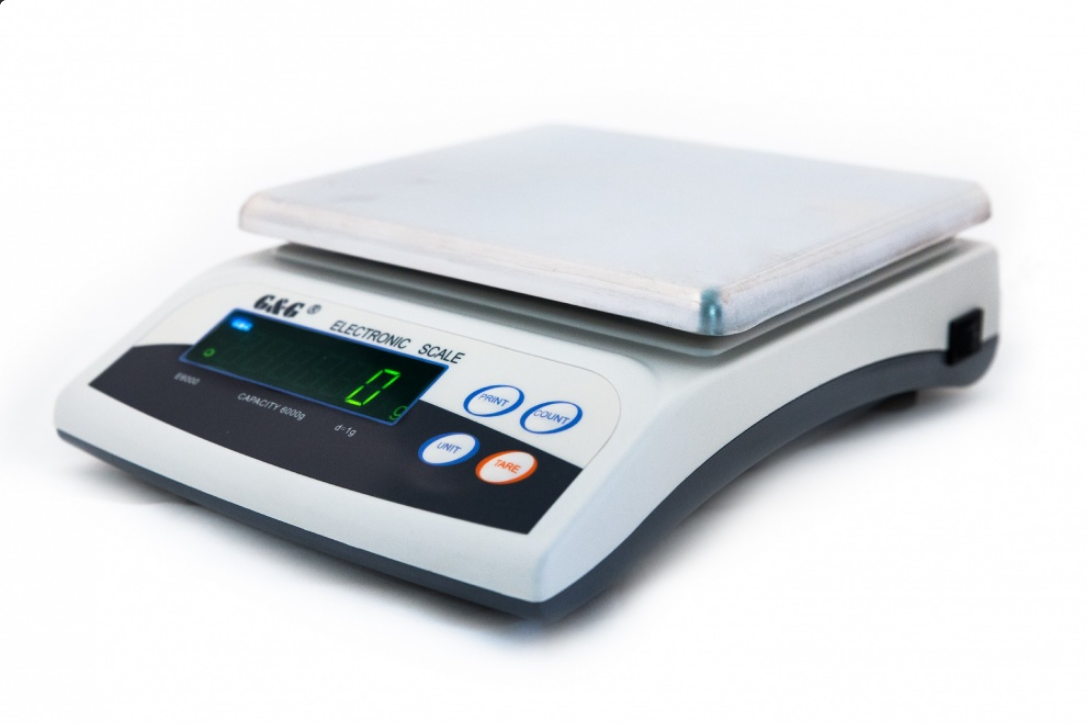
\includegraphics[scale=0.25]{obrazky/E3000.png}
    \end{center}
    \caption{Vybraná váha G\&G E3000 \cite{vaha}}
\end{figure}



% Jeden z hlavních požadavků bylo, aby váha obsahovala otevřený oboustranný komunikační port, jak pro čtení dat, tak i pro odesílání požadavků pro tisk.
% Zvolena váha disponuje RS-232 portem s komunikačním protokolem UART.

% Váživost byla volena 3Kg, protože většina větších destilátů váží do 2kg. Tudíž máme 1kg rezervu.

% Přesnost v našem případě nehraje, až tak významnou roli, proto byla váha vybírána na základě poměr "cena/výkon". Přesnost činní 0,5g.

%\subsection{Datový přenos}

%Váha posílá data přes RS-232 rozhraní. viz. kapitola č.x. Díky výstupnímu napětí 5V je možné bez nutnosti napěťového děliče připojit váhu přímo na vstup mikrokontroleru. Bohužel raspbery pi 4 disponuje pouze jedním UART rozhraním, který funguje v topologii pear-to-pear a bylo vyhrazeno pro senzor čárového kódu. Váha je tedy připojena na USB port, díky redukci RS-232 na USB, kdy propojení pinů je následovný:
%\begin{itemize}
%    \item Tx -> -D
%    \item Rx -> +D
%   \item COM -> COM
%\end{itemize}
%Napěťový vodič je pro náš systém zbytečný, proto není uvažován a datový vodiče jsou zapojený do kříže z důvodu pear-to-pear topologie.

\subsection{Datový paket vybrané váhy}
\label{datový paket váhy}

Paket se skládá z: 1x start bit, 8x datový bit, 1x stop bit.
%\begin{itemize}
%    \item 1 start bit
%    \item 8 datových bitů
%    \item 1 stop bit
%    \item bez paritního bitu
%\end{itemize}
%V našem případě není vyžadován paritní bit z důvodu opětovného odesílání stejných dat na výstup. Přínos by mohl mít pokud bychom ukládali veškeré příchozí data. Systém vezneme pouze poslední příchozí hodnotu, pokud sekvence dat za touhle hodnotou byla neměnná(např. za ±1 sekundu), tedy že se nám ustálila naměřená hmotnost.
%
%Datový paket váhy neobsahuje paritní bit, tudíž není možné zjistit zda zpráva není poškozena. Ošetření absence paritního bitu bude na SW úrovni. Pokud váha bude stabilizovaná a poslední 3 přijaté zprávy budou shodné, můžeme tuto hodnotu prohlásit/brát jako validní/správnou (nepoškozenou).

Datový paket váhy neobsahuje paritní bit, tudíž odhalení poškozené zprávy je obtížnější. Ošetření absence paritního bitu bude na softwarové úrovni, kdy se vyhodnotí poslední 3 přijaté zprávy, pokud budou všechny shodné, můžeme prohlásit, že tato hodnota je s největší pravděpodobností nepoškozená. Pravděpodobnost, že by 3x po sobě přišla stejně poškozená zpráva, je vysoce mizivá.

%Datový paket váhy neobsahuje paritní bit, což ztěžuje detekci případného poškození zprávy. Absence paritního bitu bude proto řešena na softwarové úrovni: vyhodnotí se poslední tři přijaté zprávy a pokud se všechny shodují, lze předpokládat, že jsou pravděpodobně nepoškozené. Pravděpodobnost trojnásobného opakovaného poškození stejné hodnoty je totiž téměř zanedbatelná.
%Další varianty textu: https://chatgpt.com/c/67c9adf8-0744-8000-a2f2-0d6be1335475



%\subsection{Datový rámec} %datový formát

%Datový rámec je část paketu, který obsahuje informace o hmotnosti viz. kapitola č.\ref{UARTt}. Dle dokumentace se formát skládá ze 14 bajtů zakódovaný v ASCII. Na obrázku č.\ref{data} je vidět posloupnost bajtů a jejich význam a na obrázku č.\ref{priklad} je praktický příklad.

%Datový rámec je část paketu, který obsahuje informace o hmotnosti viz. kapitola č.\ref{UARTt}. Dle dokumentace se formát skládá ze 14 bajtů zakódovaný v ASCII. Na obrázku č.\ref{data} je vidět posloupnost bajtů a jejich význam a na obrázku č.\ref{priklad} je praktický příklad.

Předpis výstupních dat se nachází v tabulce. \ref{tabos}, kdy dle dokumentace se formát skládá ze 14 bajtů zakódovaných v ASCII. V tabulce č. \ref{jouu} je praktický příklad.

%\begin{figure}[!h]
%    \begin{center}
%        \includegraphics[scale=0.5]{obrazky/data protokol - váha.PNG}
%    \end{center}
%    \label{data}
%    \caption{Předpis výstupních dat (1 unit = 1 bajt) \cite{vaha_datasheed}}
%\end{figure}

\begin{table} [!h]
    \centering
    \begin{tabular}{|l|l|l|l|l|l|}
    \hline
         Znaménko    & Mezera & Data &  Jednotka & Enter & Posun řádku \\ \hline
         1 B & 1 B           & 7 B           & 3 B &1 B&1 B\\ \hline
    \end{tabular}
    \caption{Předpis výstupních dat}
    \label{tabos}
\end{table}

%\begin{itemize}
%    \item space - "prázdný bit" %pro zachování velikosti 14-bitového slova
%    \item enter - přesunutí na začátek řádku (značení CR v ASCII: $\backslash$r)
%    \item linefeed - odřádkování (značeno LF, v ASCII: $\backslash$n) 
%\end{itemize}




\begin{table}[h]
\centering
\begin{tabular}{|p{0.6cm}|p{0.6cm}|p{0.6cm}|p{0.6cm}|p{0.6cm}|p{0.6cm}|p{0.6cm}|p{0.6cm}|p{0.6cm}|p{0.6cm}|p{0.6cm}|p{0.6cm}|p{0.6cm}|p{0.6cm}|}
\hline
\(\pm\) & SP & \multicolumn{7}{c|}{Data} & \multicolumn{3}{c|}{Jednotka} & CR & LF \\ \hline
- & \verb|␣| & \verb|␣| & 1 & 2 & 3 & . & 4 & 5 & \verb|␣| & g & \verb|␣| & \textbackslash{r} & \textbackslash{n} \\ \hline
\end{tabular}
%Pety navrhl
\caption{Příklad uspořádání dat v datovém formátu displeje}
%Můj navrh
%\caption{Příklad jak jsou data z displeje zapsány v datovém formátu}
\label{jouu}
\end{table}

\subsection{Alternativy vybrané váhy}
%Mezi alternativy k vybrané váze můžeme zařadit:
Níže je seznam s parametry vah dostupných na českém či zahraničním trhu jako alternativy k vybrané váze G\&G E3000. Váhy mají jako stejný parametr váživost 3 kg a oboustranný komunikační port RS-232, proto nejsou níže zmíněny.
\begin{itemize}
    %\item TRONIX ADX3B
    %\begin{itemize}
    %    %\item Váživost 3 kg
    %    \item Přesnost 0,1 g
    %    %\item Oboustraný komunikační port RS-232
    %    \item Cena: 2907 Kč
    %\end{itemize}
    
    \item \textbf{G\&G E3KY05}
    \begin{itemize}
        %\item Váživost 3 kg
        \item[] Výhody
        \begin{itemize}
            \item[$-$] Dostačující přesnost 0,5 g
            \item[$-$] 6 V integrovaná nabíjecí baterie
        \end{itemize}
        %\item Oboustraný komunikační port RS-232
        \item[] Nevýhody
        \begin{itemize}
            \item[$-$] Dokumentace je strohá.
            %\item Dokumentace je vysoce shodná jak u vybrané váhy G\&G E3000, proto je riziko, že by mohla být chybná
            \item[$-$] Vyšší cena: cca 3900 Kč
        \end{itemize}
    \end{itemize}
    
    \item \textbf{U.S. Solid USS-DBS86}
    \begin{itemize}
        %\item Váživost 3 kg
        \item[] Výhody
        \begin{itemize}
            \item[$-$] Dostačující přesnost 0,1 g
            \item[$-$] Nižší cena: cca 1997 Kč
        \end{itemize}
        %\item Oboustraný komunikační port RS-232
        \item[] Nevýhody
        \begin{itemize}
            \item[$-$] Dostupná pouze v zahraničí
            \item[$-$] Velice stručná dokumentace s chybějícími informacemi o komunikačním rozhraní
        \end{itemize}
    \end{itemize}
    
    \item \textbf{A\&D EK-3000i}
    \begin{itemize}
        %\item Váživost 3 kg
        \item[] Výhody
        \begin{itemize}
            \item[$-$] Dostačující přesnost 0,1 g
            \item[$-$] Obsáhlá dokumentace
            \item[$-$] Váha je certifikovaná
        \end{itemize}
        %\item Oboustraný komunikační port RS-232
        \item[] Nevýhody
        \begin{itemize}
            \item[$-$] Vyšší cena: 12670 Kč
        \end{itemize}
    \end{itemize} %G&G E3KY05 
\end{itemize}
\smallskip
Všechny výše uvedené váhy představují vhodné kandidáty pro integraci do navrženého měřicího systému. Model G\&G E3000 byl zvolen zejména s ohledem na příznivý poměr ceny a dostupnosti na tuzemském trhu. Jeho hlavní nevýhodu představuje jen stručně zpracovaná technická dokumentace.





%\begin{figure}[!h]
%    \begin{center}
%        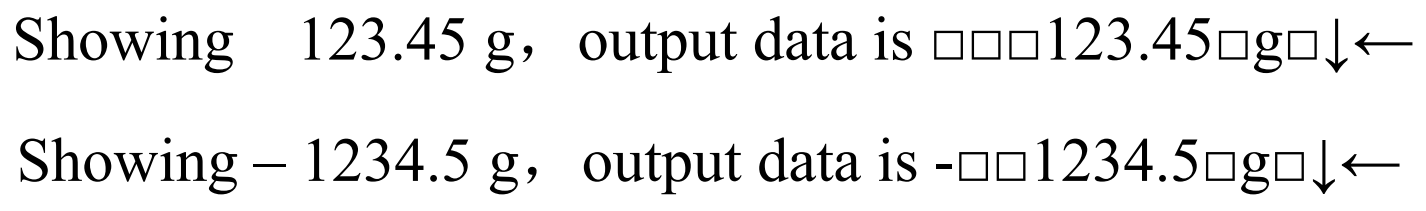
\includegraphics[scale=0.5]{obrazky/příklad protokolu - váha.PNG}
%    \end{center}
%    \label{priklad}
%    \caption{Příklad jak jsou data z displeje zapsány v datovém formátu \cite{vaha_datasheed}}
%\end{figure}



%Výstup reprezentovaný jako kod ASCII

%kombinace /r/n se vy uživa u WIndowsu k odřadkování pro 


%Vstupním portem je USB (viz. kapitola č. x), kdy piny

\section{Displej}
Další komponentou je displej, který je připojen k mikrokontroléru a zobrazuje název aktuálně měřeného destilátu, zůstatkový objem kapaliny v láhvi, maximální objem láhve, procento alkoholu měřeného destilátu a jeho obrázek pro případ, že by výrobce změnil tvar lahve, ale EAN kód by zůstal stejný.

\subsection{Požadavky na displej}
Hlavní požadavky na displej jsou:
\begin{itemize}
    \item Dotykový displej - pro budoucí implementaci klávesnice do displeje z důvodu redukce počtu periferií a snadnějšímu uživatelskému ovládání
    \item Uhlopříčka 5 - 7 palců (12,7 - 17,78 cm) pro dobrou čitelnost
    \item Bez rámečků s montážními otvory - možnost displej uchytit k vlastnímu rámu 
\end{itemize}

\subsection{Výběr displeje}

Vybraný displej je JOY-IT RASPBERRY PI touch display 7". Jeho důležité parametry jsou v tabulce č. \ref{displeej}\\

\begin{table}[!h]
    \centering
    \begin{tabular}{|c|c|}
        \hline
        Výrobce                                                         & JOY-IT   \\ \hline
        Uhlopříčka                                                      & 7" (17,78 cm)  \\ \hline
        Rozlišení                                                        & 1024 × 600 px    \\ \hline
         Rozhraní 
            & HDMI, USB \\ \hline
        Napájení & 5 V (0,6 A) \\ \hline
        Spotřeba & 3 W \\ \hline
        Dotykový displej                                                        & Ano     \\ \hline
        Cena                                                            & 2297 Kč     \\ \hline
    \end{tabular}
    \caption{Základní parametry vybraného displeje}
    \label{displeej}
\end{table}



\begin{figure}[!h]
    \begin{center}
        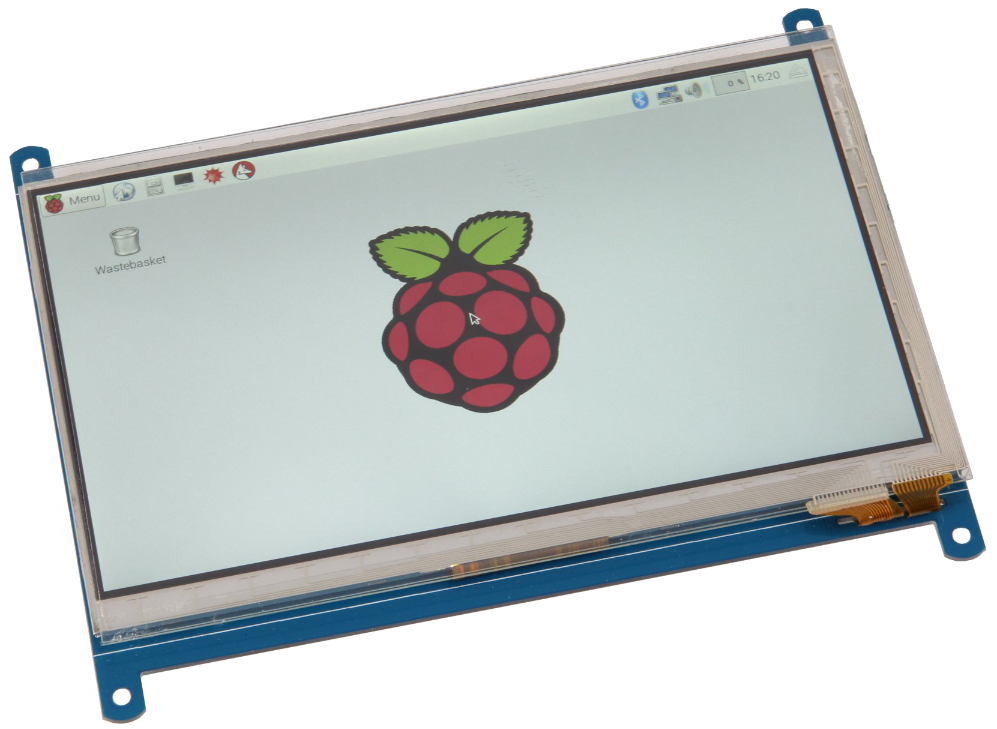
\includegraphics[scale=0.22]{obrazky/Displej.png}
    \end{center}
    \caption{Vybraný displej JOY-IT \cite{displej}}
\end{figure}



%\begin{figure}[!h]
%  \centering
%  \begin{minipage}[t]{0.46\textwidth}
%    \centering
%    \captionof{table}{Základní parametry displeje}
%    \begin{tabular}{|c|c|}
%      \hline
%      Výrobce            & JOY-IT           \\ \hline
%      Uhlopříčka         & 7″ (17,78 cm)    \\ \hline
%      Rozlišení          & 1024 × 600 px    \\ \hline
%      Rozhraní           & HDMI, USB        \\ \hline
%      Napájení           & 5 V / 0,6 A      \\ \hline
%      Spotřeba           & 3 W              \\ \hline
%      Dotykový displej   & Ano              \\ \hline
%      Cena               & 2297 Kč          \\ \hline
%    \end{tabular}
%    \label{tab:displej}
%  \end{minipage}\hfill
%  \begin{minipage}[t]{0.48\textwidth}
%    \centering
%    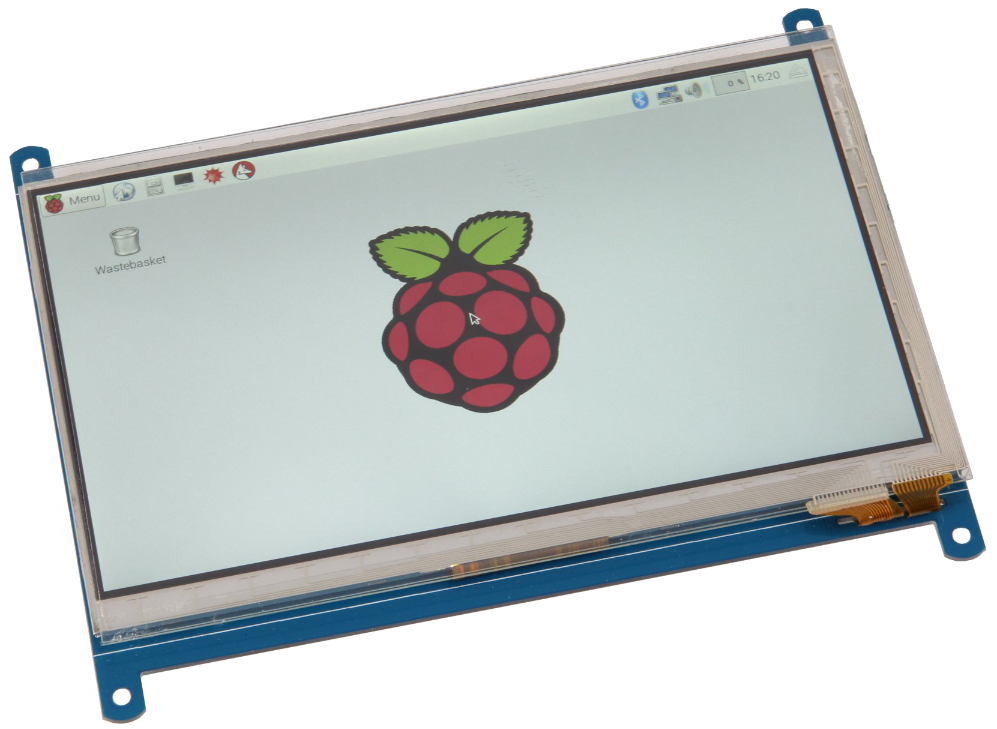
\includegraphics[width=\linewidth]{obrazky/Displej.png}
%    \captionof{figure}{Vybraný displej JOY-IT \cite{displej}}
%    \label{fig:displej}
%  \end{minipage}
%\end{figure}



\subsection{Alternativy vybraného displeje}
Mezi alternativy můžeme zařadit:
\begin{itemize}
    \item \textbf{JOY-IT RASPBERRY PI touch display 5"}
    \begin{itemize}
    \item[] Výhody
        \begin{itemize}
            \item[$-$] Montážní otvory pro uchycení displeje
            \item[$-$] Cena 1599 Kč
        \end{itemize}
    \item[] Nevýhody
        \begin{itemize}
            \item[$-$] Uhlopříčka 5" (12,7 cm)
            \item[$-$] Rozlišení 800x480 px
        \end{itemize}
    \end{itemize}
    \item \textbf{Raspberry Pi LCD - 7" Touchscreen}
    \begin{itemize}
    \item[] Výhody
        \begin{itemize}
            \item[$-$] Montážní otvory pro uchycení displeje
            \item[$-$] Cena 1399 Kč
        \end{itemize}
    \item[] Nevýhody
        \begin{itemize}
            \item[$-$] Uhlopříčka 7" (17,78 cm)
            \item[$-$] Rozlišení 800x480 px
            \item[$-$] Horší dostupnost na českém trhu.
        \end{itemize}
    \end{itemize}


    %\item JOY-IT RASPBERRY PI touch display 5" - displej se liší od vybraného menší uhlopříčkou (5"), menším rozlišením (800x480) a nižší cenou(1599 Kč)
    %\item Raspberry Pi LCD - 7" Touchscreen - displej se liší od vybraného menším rozlišením (800x480) a nižší cenou (1399 Kč). Jeho nevýhodou je horší dostupnost na českém trhu
\end{itemize}




%Displej je připojen k mikrokontroleru
%Displej nám bude zobrazovat data o 

\section{Čtečka čárového kódu}
Čtečka čárového kódu je zařízení, které, jak jeho název napovídá, umí číst grafický kód skládající se z černých a bílých proužků různých šířek, které reprezentují čísla splňující určitý standard pro obchodní průmysl, jako je například formát EAN. EAN (European Article Number) je mezinárodní unikátní identifikační číslo, které usnadňuje prodejcům prodej zboží. Pro český trh se běžně využívá EAN-13 (13-ti místné číslo nacházející se pod čárovým kódem). 

Čárové kódy se dělí na jednorozměrné (1D, lineární), které běžně známe z produktů v obchodech (černobílé proužky) a dvojrozměrné (2D) reprezentované jako matice bodů. Nejznámějším 2D formátem je QR (Quick Response) kod, který se využívá k rychlému placení, sdílení URL adres, připojení k internetu, atd. V praxi jsou 1D kódy, uloženy v databázi obchodu, ke kterému je přiřazen název a cena produktu.
%Čtečka čárového kódu je zařízení, které, jak jeho název napovídá, umí číst kód skládající se z černých proužků různých délek \cite{carovy_kod}, které reprezentují čísla splňující EAN standard.
%zdroj1: https://pageloot.com/cs/carovy-kod/jak-funguje-skener-carovych-kodu/
%zdroj2: https://cs.wikipedia.org/wiki/%C4%8Cte%C4%8Dka_%C4%8D%C3%A1rov%C3%A9ho_k%C3%B3du

%EAN (European Article Number) je mezinárodní unikátní identifikační číslo, které usnadňuje prodejcům prodej zboží. Pro český trh se běžně využívá EAN-13 (13-ti místné číslo nacházející se nad čárovým kódem) \cite{EAN}
%zdroj: https://cs.wikipedia.org/wiki/European_Article_Number

%V praxi je toto číslo uloženo v databázi obchodu, které je spojeno s název produktu a jeho cenou. Po načtení čárového kódu. %Po načtení čárového kódu

%V praxi je toto číslo uloženo v databázi obchodu, ke kterému je přiřazen název a cena produktu.

%Každé zboží se dá lehce indetifikovat pomocí

%V této sekci se nebudeme zabývat, jakým způsobem jsou čísla kódována do této podoby, ale jakým způsobem lze tyto čárové kódy číst.

Čárový kód se skládá z ochranných znaků „start“ a „stop“, ze středového dělícího znaku a z datových znaků, které reprezentují jednotlivé číslice. Formát EAN‑13 konkrétně určuje, že první tři číslice (tzv. prefix) značí zemi nebo region registrace, následujících šest jich slouží k identifikaci výrobce a dalších pět k rozlišení konkrétního produktu. Poslední třináctá číslice má kontrolní charakter. Vypočteme ji tak, že od konce kódu sčítáme číslice (kontrolní číslici ignorujeme) na lichých pozicích (1., 3., 5. atd.). Získaný součet vynásobíme trojkou, potom přičteme součet číslic, které leží na sudých pozicích. Výsledné číslo odečteme od nejbližšího vyššího násobku deseti a takto získaný rozdíl je kontrolní číslice. Tento postup pomáhá ověřit správnost EAN‑13 a minimalizuje chyby při skenování. [zdroj1][zdroj2]
%Zdroj1: https://is.ambis.cz/th/jmeqf/BP_Carove_kody_MMachan_3BK_IT.pdf
%Zdroj2: https://www.vut.cz/www_base/zav_prace_soubor_verejne.php?file_id=16877

\begin{figure}[!h]
    \begin{center}
        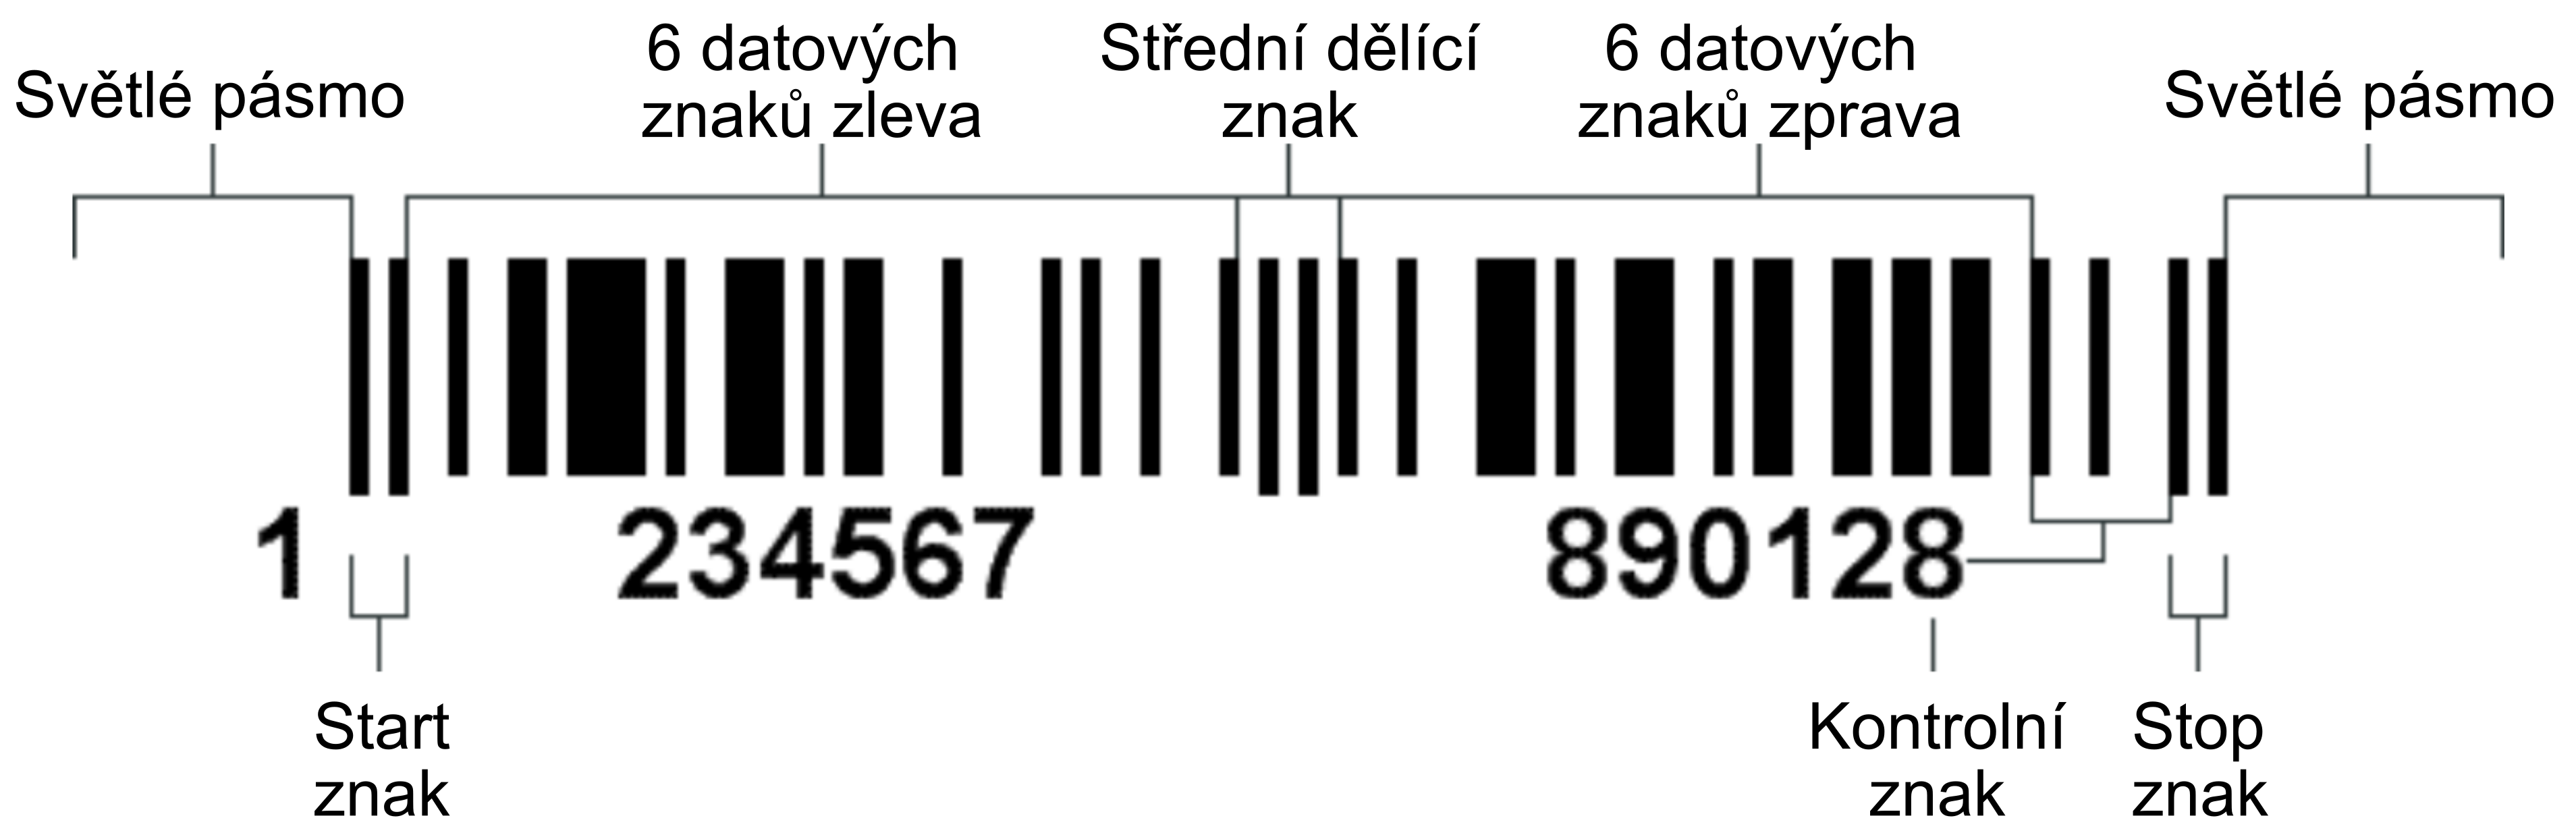
\includegraphics[scale=0.15]{obrazky/čárový kód.png} %0.5
    \end{center}
    \caption{Ukázka čárového kódu EAN-13.}
    \label{čárový kod}
\end{figure}





\subsection{Požadavky na čtečku čárového kódu}
Na trhu existuje celá řada čteček lišících se přesností, způsobem implementace a velikostí. Pro navrhovaný systém je vyžadována čtečka bez ochranného krytu s montážními otvory nebo s dostatečným prostorem pro jejich vyvrtání, aby čtečku bylo možné integrovat do vlastní konstrukce (krabičky) společně se všemi dalšími komponenty. Přednost se dává technologii CCD nebo kamerovému snímači díky vyšší mechanické odolnosti (např. při pádu) a lepší čitelnosti částečně poškozených kódů.
V poslední řadě je nutné, aby čtečka zvládala číst EAN-13 a méně často používaný EAN-8.

%dodelat zde tabulku: technologie: Kamerove (cmos), typ kodu: 1D, 2D, rychlost čtení, proudový odběr


%Na trhu je dostupných více druhů senzorů, které se liší požadavky na přesnost, druh implementace, velikostí atd. Velikost se požaduje menší bez ochranné krabičky pro budoucí uchycení do navrhnuté krabičky, která zastřeší všechny komponenty systému na jednom místě. včetně montážních otvorů nebo dostatečného prostoru pro jejich vyvrtání. Preferovanou technologií je CCD nebo CMOS z důvodu větší durability např. při pádu měřícího systému na zem a lepší čitelnosi poškozených kódů. Navíc od roku 2025 by mělo z obchodník řetězců vymizet klasické 1D čárové kódy a měli by je nahradit 2D QR kody, otázkou je zda přibude i nový formát 2D kódů na kterou budou vyvýjeny nové čtecí systémy

%Požaduje se komunikační rozhraní, nejlépe USB nebo UART pro odesílání a přijímání dat ze čtečky. Datový formát nejlépe ASCII, stejně jako u vybrané váhy, pro jeho jednoduché zpracování.

%Komunikační rozhraní čtečky se požaduje UART nebo USB s možností povolení virtuálního seriového portu pro komunikaci s mikrokontrolérem - označováno USB VCom.

%Další požadavek spočívá v tom, aby čtečka byla schopna číst standard EAN-13, který je běžně používán v České republice, a také EAN-8, s nímž se lze výjimečně setkat.
\subsection{Vybraná čtečka čárového kódu}

%Vybraná čtečka je GM65 od společnosti KROW, využívající CMOS technologie, obrázek č.\ref{gm65}.
%Čtečka disponuje UART a USB VCom. Kompletní specifikace je obsažena v dokumentaci.\cite{scaner}
%Datový formát pro seriovou komuniaci čtečky je stejný jak u vybrané váhy[xx] i zde chybý ověřovací bit, který bude ošetřen softwarově

%Z důvodu technologického pokroku a podle výše zmíněných parametrů jsem byl schopen najít pouze CMOS čtečky, proto tedy vybraná čtečka je GM65....

S ohledem na výše uvedené požadavky byla vybrána kamerová čtečka KROW GM65, využívající optických snímačů CMOS (viz obrázek č.\ref{gm65}) a LED diody pro nasvícení čárového kódu v hůře osvětleném prostředí. Čtečka nabízí komunikační rozhraní UART a USB. Datový formát pro sériovou komunikaci je shodný s vybranou váhou [\ref{datový paket váhy}].
%Podobně jako u váhy chybí ověřovací bit, který bude řešen softwarově. Podrobné technické specifikace čtečky jsou uvedeny v její dokumentaci.

\begin{table}[!h]
    \centering
    \begin{tabular}{|c|c|}
        \hline
        Výrobce                & KROW             \\ \hline
        Model                  & GM65             \\ \hline
        Typ                    & Kamerová čtečka  \\ \hline
        Čtecí vzdálenost \tablefootnote{Pro standard EAN-13 s šířkou kódu 35,6 mm při intenzitě osvětlení 250 lux}       & 4 - 25 cm            \\ \hline
        Rozhraní & HDMI, USB \\ \hline
        Napájení               & 5 V (až 160 mA)  \\ \hline
        Spotřeba               & 0,8 W            \\ \hline
        Rychlost čtení         & 0,1 s            \\ \hline
        Cena                   & 992 Kč           \\ \hline
    \end{tabular}
    \caption{Základní parametry vybraného displeje}
    \label{displeej}
\end{table}


\begin{figure}[!h]
    \begin{center}
        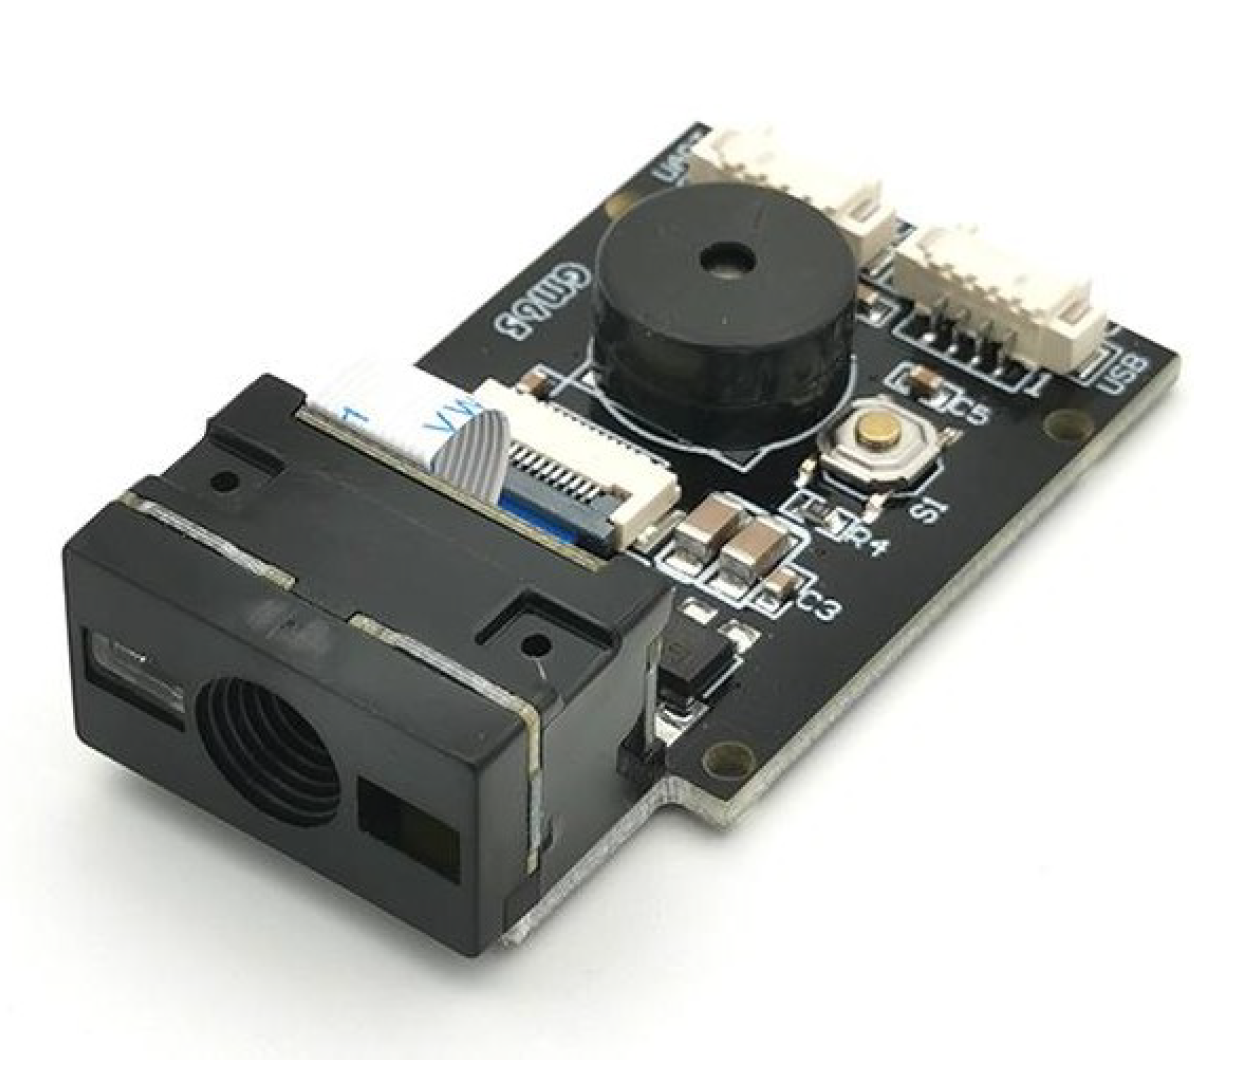
\includegraphics[scale=0.25]{obrazky/gm65.PNG} %0.5
    \end{center}
    \caption{Vybraná čtečka čárového kódu KROW GM65 \cite{scaner}}
    \label{gm65}
\end{figure}

%Toto níže je blbost
%\begin{table} [!h]
%    \centering
%    \begin{tabular}{|l|l|l|l|l|l|}
%    \hline
%         Hlavička  & Typ & Délka dat & Adresa & Data & CRC \\ \hline
%         2 B       & 1 B & 7 B       & 3    B & 1 B  & 1 B\\ \hline 
%    \end{tabular}
%    \caption{Předpis výstupních dat}
%    \label{datovy format čtečky}
%\end{table}




\subsection{Alternativy vybrané čtečky čárového kódu}
%Mezi alternativy můžeme zařadit:
%Vybrané alternativy jsou kamerové

\begin{itemize}
    \item YHDAA YHD-M800D
    \begin{itemize}
        \item[] Výhody
        \begin{itemize}
            \item[$-$] Typ: Kamerový snímač
            \item[$-$] Cena: 1000 Kč
            \item[$-$] Rozhraní: USB
        \end{itemize}
        \item[] Nevýhody
        \begin{itemize}
            \item[$-$] Nepřehledná a nevypovídající dokumentace
        \end{itemize}
    \end{itemize}
    \item WaveShare Barcode Scanner
    \begin{itemize}
        \item[] Výhody
        \begin{itemize}
            \item[$-$] Typ: Kamerový snímač
            \item[$-$] Rozhraní: USB, UART
        \end{itemize}
        \item[] Nevýhody
            \begin{itemize}
                \item[$-$] Vyšší cena: 1318 Kč
            \end{itemize}
    \end{itemize}
\end{itemize}
\smallskip
Vhodnou alternativou je WaveShare, která nabízí srovnatelné technické parametry jako aktuálně zvolený model. V obou případech je k dispozici kvalitní a podrobná dokumentace. Výběr čtečky nakonec připadl na KROW GM65 z důvodu nižší ceny.



%\begin{itemize}
  %  \item YHDAA YHD-M800D - kamerová čtečka, cenově stejně dostupné(1000 Kč) jak vybraná čtečka, integrovaný USB port, nepřehledná a nevypovídající dokumentace 
 %   \item WaveShare Barcode Scanner - kamerová čtečka, dražší než vybraná čtečka(1318 Kč), integrovaný sériový port micro USB a UART
%\end{itemize}

\section{Modul s výpočetní jednotkou} %Mikrokontroler
%Výpočetní modul / Modul s výpočetní jednotkou / Řídicí jednotka / Výpočetní jednotka

Modul s výpočetní jednotkou je samostatná hardwarová součást (obvykle deska plošných spojů osazená procesorem, pamětí a potřebnými rozhraními), která ve větším elektronickém či řídicím systému zajišťuje hlavní výpočetní výkon. Často pracuje v kombinaci s jinými moduly – sběrnicovými, vstupními (senzory, klávesnice), výstupními (displeje, motory) nebo dalšími výpočetními jednotkami. Mezi běžné představitele těchto výpočetních jednotek patří:
\begin{itemize}
    \item Mikrokontrolery (Jednočipové PC, MCU): Jsou to systémy na jednom čipu, které integrují procesor, paměť flash a RAM, A/D převodník, oscilátor (hodiny) a I/O porty. Běžně se využívají v real-time aplikacích, jež nevyžadují vysoký výpočetní výkon.
    \item Jednodeskové počítače (SBC, mikropočítače): Vyšší stupeň integrace oproti mikrokontrolérům. Jde o plnohodnotné počítače na jedné desce. Obvykle běží pod operačním systémem a nabízejí více periferií, což je činí vhodnými pro komplexní a výpočetně náročnější úlohy.
\end{itemize}


%Mikrokontroler jinak označovaný jednočipový počítač je integrovaný obvod
%Mikrokontrolér nebo také jednočipový počítač je integrovaný obvod obsahující kompletní mikropočítač. Jednočipové počítače se vyznačují velkou spolehlivostí a kompaktností, proto jsou určeny především pro jednoúčelové aplikace. Mikrokontroléry jsou často používány v embedded systémech, jako jsou například řídicí systémy, regulátory, senzory a další aplikace, kde je potřeba rychle a spolehlivě zpracovávat data. V praxi si můžeme pod takovou řídicí jednotkou představit např. PLC (Programovatelný automat)
%[zdroj]
%Na bakalařku překopat...je to opsaný
%https://sk.wikipedia.org/wiki/Mikrokontrol%C3%A9r
%https://cs.wikipedia.org/wiki/Jedno%C4%8Dipov%C3%BD_po%C4%8D%C3%ADta%C4%8D

\subsection{Požadavky na modul s výpočetní jednotkou} %Požadavky na řídicí jednotku / výpočetní modul
%napájení
%OS(bez os nepojede databaze atd) a grafická čip, hdmi,  pro vývoj GUI
%Jednodeskotopový PC skrz chod pythonu a Tkinter, ten na mikrokontroleru nerozjedu skrz malou pamět a výkon a na MikroPython nic takového nebude. Dále mikrokontorler nemá SD slot pro ukládání databáze
%V mobilu mam napsany od petyho proč nevybrat to a tam a nejaky popis k mikrokontrolerum

%

Hlavním z požadavků je snadná realizovatelnost firmware s integrovaným grafickým uživatelským rozhraním (GUI) ovládaného dotykovým displejem. Pro takové účely je vhodné použít vysokoúrovňový programovací jazyk, např. Python, který nabízí široký výběr knihoven a nástrojů, které ulehčují a zrychlují vývoj samotného firmware, na druhou stranu je nutné přihlédnout na dostačující výkon a operační paměť (RAM) řídicí jednotky. Vývoj GUI a práce s databází obnáší zpravidla přítomnost OS už jen z důvodu zabudovaných grafických ovladačů pro komunikaci s displejem, správu paměti nebo využití grafických knihoven, které je pro svoji funkčnost OS vyžadují, proto využiji nenáročné distribuce linuxu, která je oproti konkurenčním OS výkonově i paměťově nenáročná.
%Z důvodu volby vysokoúrovňového programovacího jazyku, GUI a využití databáze je nutné, aby firmware běžel na OS.
%Z důvodu minimální výkonové a paměťové náročnosti poběží řídicí jednotka na nenáročné distribuci Linuxu. Pro takový účely se hodí libovolná distribuce linuxu, která je hojně využívána u jednodeskových počítačů.

Další požadavky:
\begin{itemize}
    \item Výkon a paměť: 
        \begin{itemize}
            \item Dostatečně výkonný procesor pro chod GUI aplikace.
            %\item Dvou a více jádrový procesor pro paralelní chod GUI a stavového automatu pro zpracování dat ze čtečky čárového kódu a váhy. 
            %\item Minimální velikost RAM paměti 2 GB, optimálně 4-8 GB pro plynulý chod GUI a OS.
            \item Velikost paměti RAM optimálně 2 GB pro plynulý chod GUI a OS.
        \end{itemize}
    \item Periferie:
        \begin{itemize}
            \item 3x USB-A (optimálně verze 3.0) pro čtečku čárového kódu, váhu a napájení displeje. Výstupní proud alespoň 0,6 A 
            \item 1x HDMI nebo Micro HDMI pro dotykový displej
            \item slot na SD kartu na které bude uložen firmware, databáze, atd.
            
            %\item slot na SD kartu na které budou uložena veškerá data databáze zmíněná v kapitole č. 5.3, operační systém a samotný firmware. Velikost SD karty alespoň 32 GB[zdroj1] pro plynulý chod OS 
            
            %pro optimální rychlost čtení a zápisu [zdroj1][zdroj2]. %Například pro Rasbian OS (OS jednodeskových počítačů(SBC) raspberry pi) je doporučovaná velikost minimálně 4 GB[Zdroj1]
            %Zdroj1 : https://www.raspberrypi.com/documentation/computers/getting-started.html
            %Zdroj2 : https://www.raspberrypi.com/documentation/accessories/sd-cards.html
            \item řídicí jednotka musí zvládnout poskytnout dle vybraných komponent, alespoň 0,7 A při 5 V, optimálně 1,2 A, pro případ rozšíření systému o další komponenty.
            %\item Alespoň jeden GPIO pro ovládání pípáku
        \end{itemize}
    \item Integrovaný Wi-Fi modul: Do budoucna je cílem bezdrátová konektivita s měřicím systémem pomocí mobilní aplikace nebo připojení k ERP systémům
    %\item napájení/odběr/příkon/spotřeba: ...
    %Výstupní proud 0,6 A (USB): Výkonově nejnáročnější komponentou připojené k řídicí jednotce bude displej[] s proudovým odběr 0,6 A při 5 V. (Do budoucna bude měřicí systém bude obsahovat baterii, který může napájet jednotlivé komponenty.) Pro provoz displeje, který je proudově nejnáročnější je nutné, aby USB porty dokázaly poskytnout minimálně 0,6 A při 5 V. řídicí jednotka musí zvládnout poskytnout dle vybraných komponent, alespoň 0,7 A při 5 V, optimálně 1,2 A, pro případ rozšíření systému o další komponentu.
\end{itemize}

%Nevybírat model s konrétní velikost ram, ale určit více velikostí a pak podle toho dát rozsah ceny
\subsection{Vybraný modul s výpočetní jednotkou}
Na základě výše zmíněných požadavků byl vybrán jednodeskový počítač Raspberry Pi 4 ve verzi s 4 GB operační paměti. Kategorii mikrokontrolérů jsem úplně vynechal z důvodu nedostatečného výkonu a operační paměti pro chod OS s GUI aplikací a absence integrovaných periférií jako USB nebo HDMI. 

Mezi klíčové výhody Raspberry Pi patří široká komunita, kvalitní podpora i bohatá škála dokumentace a knihoven. Další z výhod je rozumný poměr cena výkon a spolehlivost. Základní technické parametry jsou přehledně uvedeny v tabulce č. \ref{raspbericko_spec}, zatímco kompletní specifikace lze nalézt v příslušné dokumentaci. \cite{Raspberry pi}

%Vyrobce
%Model
%Procesor
%RAM
%Rozhraní 2x USB 2.0, 2x USB 3.0, 2x HDMI 1.4 (asi)
%Napájení 5V DC
%Spotřeba 4 - 7 W
%Dále obsahuje: Wi-Fi/BT modul, SD slot, 3,5 mm Jack


\begin{table}[H]
    \centering
    \begin{tabular}{|c|c|}
        \hline
        Výrobce                                                         & Raspberry Pi Foundation   \\ \hline
        Model                                                           & Raspberry Pi 4  \\ \hline
        %\begin{tabular}[c]{@{}c@{}}Komunikační\\ protokol\end{tabular}  & UART   \\ \hline
        CPU & \begin{tabular}[c]{@{}c@{}}1.5GHz čtyřjádrový \\ ARM Cortex-A72\end{tabular} \\ \hline
        GPU & VideoCore VI 500 MHz \\ \hline
        RAM & 4 GB \\ \hline
        Periferie & \begin{tabular}[c]{@{}c@{}} 2x USB-A 3.0 \\ 2x USB-A 2.0 \\ 1x USB-C (napájení) \\ 2x microHDMI 2.0 \\ 1x Gigabit Ethernet \\ 40x GPIO \end{tabular} \\ \hline
        Napájení                                                        & 5 V DC (až 3 A)   \\ \hline
        Spotřeba                                                        & 3 - 7 W     \\ \hline
        Dale obsahuje & \begin{tabular}[c]{@{}c@{}} Wi-Fi/BT modul \\ SD slot \end{tabular} \\ \hline
        Cena                                                            & 1987 Kč     \\ \hline
    \end{tabular}
    \caption{Základní parametry Raspberry Pi 4 \cite{Raspberry pi}}
    \label{raspbericko_spec}
\end{table}

%Hlavní nevýhodou je pořizovací cena 1479 Kč a vyšší spotřeba energie v rozmezí 3 - 7 W. Kompletní specifikace se nachází v dokumentaci výrobce.[2]



%Vybraný mikrokontroler byl Raspberry PI 4, který dokáže pokrýt veškeré požadavky na měřicí systém. Konkrétně se jedná o model B s 4 GB operační paměti. Zde jsou zmíněné požadavky na mikrokontrolér:

%\begin{itemize}
%    \item Dostatečný počet portů pro připojení všech modulů.
%    \item Integrovaná čtečka SD karty pro ukládání databáze
%    \item Dostatečný výkon pro chod GUI aplikací. Do budoucna je v plánu implementovat dotykový displej, na kterém budou veškeré informace pěkně přehledné díky grafickému rozhraní
%    \item Integrovaný čip pro bezdrátovou konektivitu. Do budoucna možnost vývoje mobilní aplikace k vyvíjenému systému nebo bezdrátové připojení k ERP systémům.
%    \item
%    \item Hlavní z požadavků je snadná realizovatelnost firmware s integrovaným grafickým uživatelským rozhraním pro ovládání dotykového displeje. Pro takový účely je vhodné použít programovací jazyk Python, který nabízí širší výběr knihoven a nástrojů, které ulehčují a zrychlují vývoj samotného firmware.
%
%    \item
%\end{itemize}
%Dost požadavků je nad rámec bakalářské práce, ale pro budoucí inovaci systému nemusíme měnit mikrokontrolér a realizovat znovu už fungující HW kompatibilitu mezi komponenty a vyvíjet SW vybavení.

%Jedinou nevýhodou je vysoká pořizovací cena.

\begin{figure}[H]
    \begin{center}
        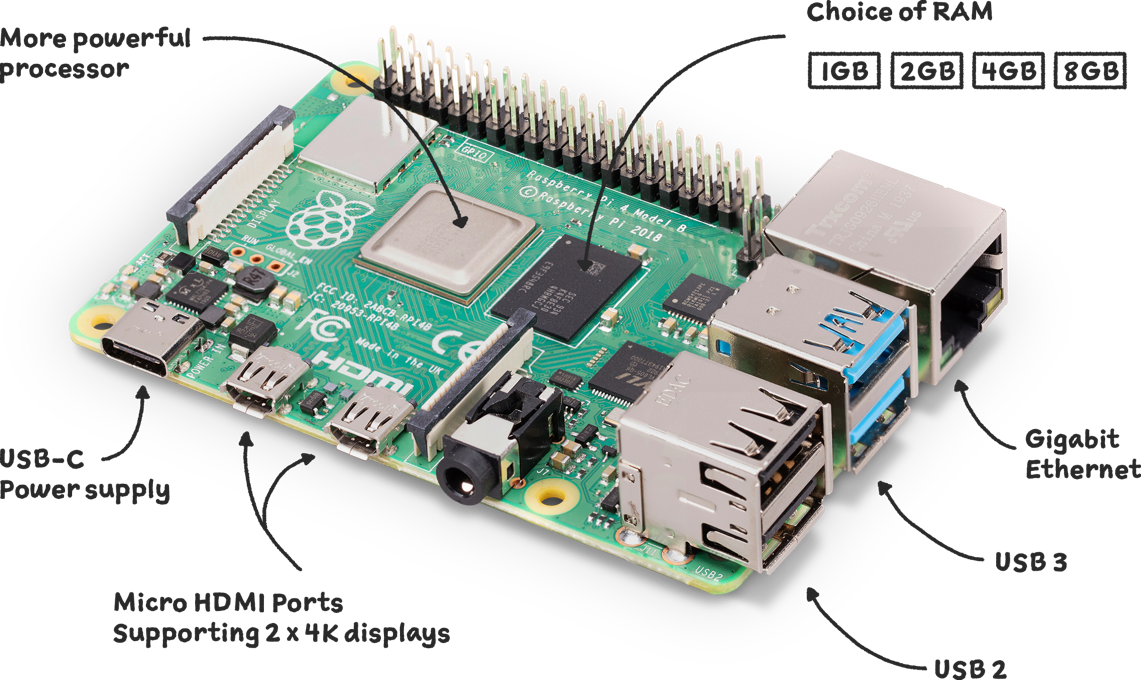
\includegraphics[scale=0.3]{obrazky/raspberry-pi-4.png}
    \end{center}
    \caption{Vybraný jednodeskový PC Raspberry Pi 4 \cite{malina_obr}}
    %\label{gm65}
\end{figure}

\subsection{Alternativy vybraného modulu s výpočetní jednotkou}
Níže je seznam alternativ, včetně výhod a nevýhod vůči vybranému mikropočítači Raspberry Pi 4. Všechny ceny jsou orientační pro rok 2024.

%Raspberry piko
%Arduino Uno
%Esp 32 (SoC/mikrokontroler + WIFI/BT)
%Acemagic T8-PRO N5105 (8+0) Silver (Přebustěny jednodeskový pc / mini PC)

\begin{itemize}
    %\item \textbf{ESP32} (MCU)
    %    \begin{itemize}
    %        \item Výhody
    %            \begin{itemize}
    %                \item asdasd
    %                \item asddd
    %            \end{itemize}
    %        \item Nevýhody
    %        \begin{itemize}
    %            \item fdf
    %            \item fff
    %        \end{itemize}
    %        \item Zlomová cena - 200 Kč
    %        \item Absence debuggeru
    %        \item ...
    %    \end{itemize}
    \item \textbf{Banana Pi M5} (Druhá nejlepší volba)
        \begin{itemize}
        \item[] Výhody
            \begin{itemize}
                \item[$-$] Výkonnější procesor - Cortex-A55 (4 jádra, 2 GHz)
                \item[$-$] Integrované uložiště eMMC (rychlejší než SD karta)
                \item[$-$] Nižší cena: cca 2000 Kč.
            \end{itemize}
        \item[] Nevýhody
            \begin{itemize}
                \item[$-$] Horší dostupnost v lokálních obchodech (často nutný dovoz). To sebou nese i problémy s reklamací.
                \item[$-$] Menší uživatelská základna - méně zdrojů, tutoriálů a komunitních projektů.
                \item[$-$] Kopie Raspberry Pi 4 - Potenciálně menší životnost HW, možné problém s licencemi (např. GPL).
            \end{itemize}
        \item[] Zhodnocení: Pokud by primární volba byla nedostupná, představuje Banana Pi M5 realistickou náhradu při zachování požadovaného výkonu i rozhraní, avšak za cenu vyššího rizika dlouhodobé podporovatelnosti.
        \end{itemize}
    \item \textbf{Odroid XU4}
        \begin{itemize}
        \item[] Výhody
            \begin{itemize}
                \item[$-$] Integrované uložiště eMMC (rychlejší než SD karta)
                \item[$-$] Nižší cena: cca 2000 Kč.
            \end{itemize}
        \item[] Nevýhody
            \begin{itemize}
                \item[$-$] Absence Wi-Fi modulu (možnost externího připojení).
                \item[$-$] Pouze 2 GB RAM.
                \item[$-$] Komunita je relativně aktivní, ale stále menší než u Raspberry Pi.
            \end{itemize}
        \end{itemize}
    %- Jen 2 GB RAM. Nemá integrovaný Wi-Fi modul, nutnost připojit externě.
    \item \textbf{NVIDIA Jetson Nano} 
        \begin{itemize}
            \item[] Výhody
            \begin{itemize}
                \item[$-$] Vysoký grafický výkon. Vhodnější pro strojové učení a práci s AI. Pro navrhovaný systém nevyužitelný.
            \end{itemize}
            \item[] Nevýhody
            \begin{itemize}
                \item[$-$] Absence Wi-Fi modulu (možnost externího připojení)
                \item[$-$] Vyšší spotřeba 7 - 24 W
                \item[$-$] Vyšší cena: cca 8000 Kč.
            \end{itemize}
        \end{itemize}
    \item \textbf{Recyberry Asus Tinker Board S.} 
        \begin{itemize}
            \item[] Výhody
            \begin{itemize}
                \item[$-$] Integrovaný eMMC (rychlejší načtení OS)
            \end{itemize}
            \item[] Nevýhody
            \begin{itemize}
                \item[$-$] Aktuálně nedostupný na českém trhu%Horší dostupnost v lokálních e-shopech
                \item[$-$] RAM 2 GB.
                \item[$-$] USB 2.0 (10x pomalejší než USB 3.0 
                %[zdroj: to co useriove komunikace])
            \end{itemize}
        \end{itemize}
    %\item Recyberry Asus Tinker Board 2S - Vyší napájecí napětí 12-19 V, 
    %\item Arduino Portenta X8 - Nemá nativní HDMI port, ale zde využít USB-C konektoru jako Displey Port a pro ostatní USB porty použít USB rozbočovač
\end{itemize}




%Rozhodoval jsem se mezi dalšími dvoumi 







%proč malinu:
%
%-graficky čip pro dotykovy displej, 
%
%-wifi/BT čip pro budouci mobilni aplikaci, 
%
%-možnost vývoje GUI (python, CS) bezne mikrokontrole funguje jen na C/C++ asi,
%
%-rozumně velké uložiště pro ("GUI aplikaci" spíš RAM) databázi, která se časem bude rozšiřovat nevim jestli by arduino to pojmulo, ale určitě arduino nepojme databází obrázků, jednotlivých destilátů
%%https://www.dps-az.cz/clanky/id:6173/uvod-do-embedded-systemu
\chapter{Zprovoznění jednotlivých komponent}
\label{Zprovoznění jednotlivých komponent}
Jednotlivé komponenty jsou připojeny k mikrokontroléru podle obrázku č. \ref{blokove_schema}. Displej a klávesnici stačí jen připojit, proto je nebudu v rámci této kapitoly více rozebírat.

\section{Ověření přesnosti váhy}

Před použitím samotné váhy jsem ověřil, zda její přesnost odpovídá parametrům stanoveným výrobcem z důvodu, že váha není certifikovaná. Ověření probíhá pomocí druhé váhy nebo kalibrovaného závaží o jednu třídy přesnosti výše. Pro váhu integrovanou do měřícího systému G\&G E3000 je třída přesnosti III, proto je nutné volit váhu s třídou přesnosti II dle normy OIML R 76 nebo kalibrované závaží s třídou přesnosti M1 dle normy OIML R 111. Pro ověření přesnosti byla použita váha Kern PCB-2500-2 s padesátkrát vyšší přesností: 0,01 g a váživostí 2,5 kg. Obě váhy byly před použitím kalibrovány a použity v laboratorním prostředí s teplotou 20,4 °C a vlhkostí 28,7 \%, které odpovídají požadavkům obou výrobců vah pro přesná měření. Z tabulky č. \ref{tab:vahy} je vidět, že váha G\&G-3000 měří s požadovanou přesností 0,5 g. %a spadá tak do třídy přesnosti III.




%\begin{table}
%    \centering
%    \begin{tabular}{|c|c|}
%    \hline
%         \begin{tabular}[c]{@{}c@{}} Kern PCB-2500-2 \\ (g) \end{tabular} & \begin{tabular}[c]{@{}c@{}} G\&G E3000 \\ (g) \end{tabular}\\ \hline
%         20,00 & 20,0\\ \hline
%         200,00&200,0 \\ \hline
%         400,00&400,0 \\ \hline
%         600,00 & 600,0 \\ \hline
%         800,00&800,0 \\ \hline
%         1000,00&1000,0 \\ \hline
%         1200,00&1200,0 \\ \hline
%         1400,00&1400,0 \\ \hline
%         1600,00&1600,0 \\ \hline
%         1800,00&1800,0 \\ \hline
%         2000,00&2000,0 \\ \hline
%         2200,00&2200,0 \\ \hline
%    \end{tabular}
%    \caption{Ověření přesnosti váhy G\&G E3000}
%    \label{tab:vahy}
%\end{table}

\begin{figure}[H]
    \begin{center}
        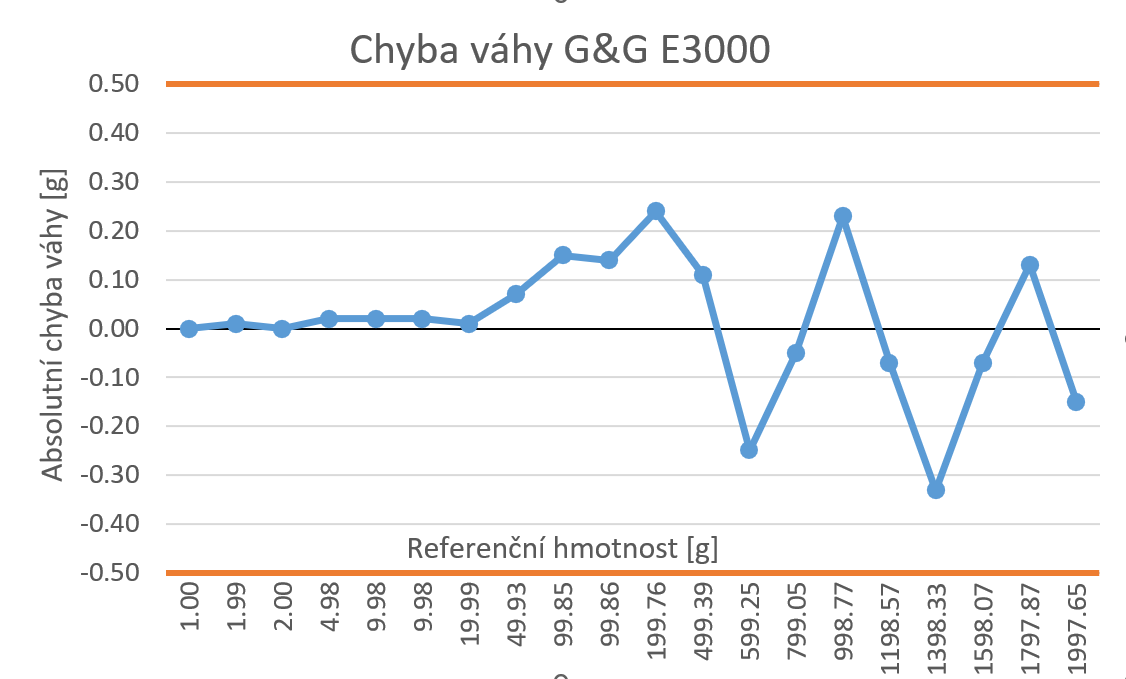
\includegraphics[scale=0.7]{obrazky/mereni.PNG}
    \end{center}
    \caption{Nalevo Kern PCB-2500-2, napravo G\&G E3000}
    \label{adapter}
\end{figure}

\begin{figure}[H]
    \begin{center}
        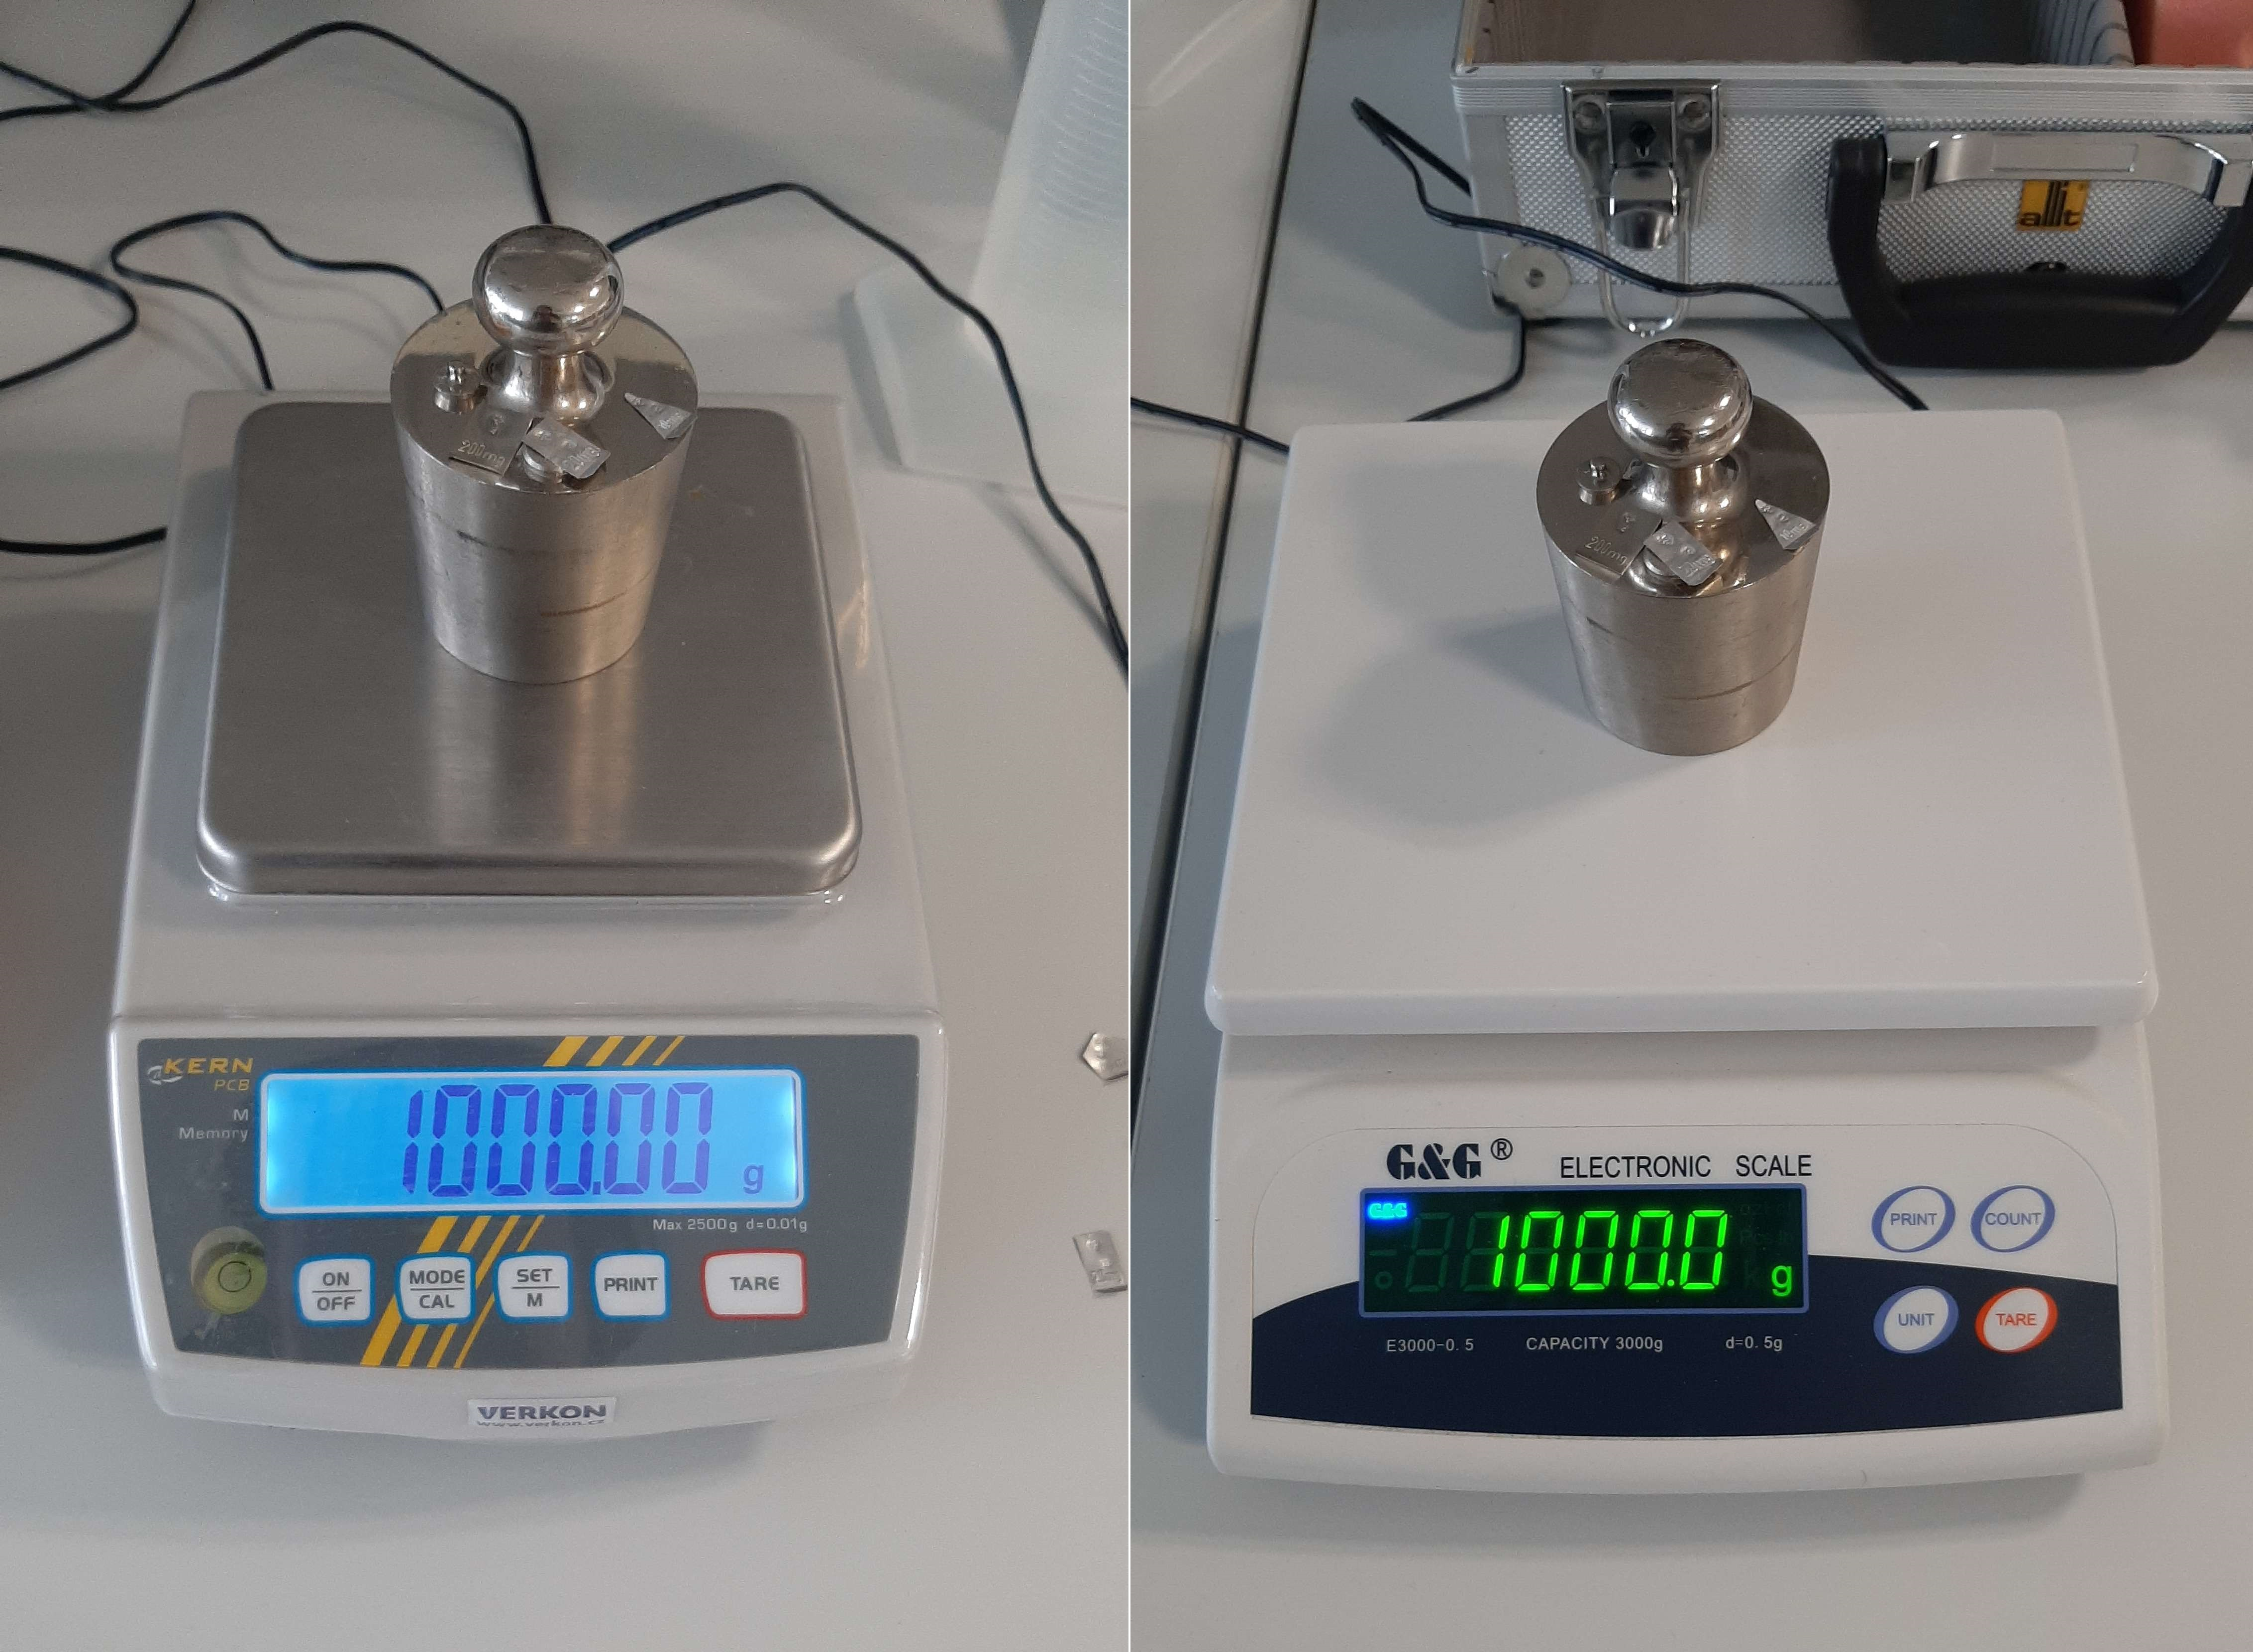
\includegraphics[scale=0.1]{obrazky/vahy.jpg}
    \end{center}
    \caption{Nalevo Kern PCB-2500-2, napravo G\&G E3000}
    \label{adapter}
\end{figure}

\section{Zprovoznění váhy}

Komunikační rozhraní váhy je RS-232, který nejsme schopni připojit na mikrokontrolér z důvodu absence totožného rozhraní. V takovém případě použijeme adaptér z RS-232 na USB. Použitý adaptér je ADS-50 USB - serial, který je součástí balení váhy (obrázek č.\ref{propojení váhy v1}).

%\begin{figure}[H]
%    \begin{center}
%        \includegraphics[scale=0.06]{obrazky/ADS-50 USB - serial adapter.png}
%    \end{center}
%    \caption{Adaptér USB - serial AXAGO ADS-50}
%    \label{adapter}
%\end{figure}

Propojení kabelu ADS-50 s váhou není možné z důvodu, že kabel není křížený, jinak zvaný "null modem" kabel. To znamená, že vysílací piny(Tx) jsou navzájem propojené a to samé přijímací piny(Rx). Aby komunikace mohla fungovat je nutné propojit Tx s Rx. Tato podmínka komunikace je zmíněná v dokumentaci váhy[x]. Výrobce váhy z tohoto důvodu k balení přidal kříženou redukci DB9(samice) - DB9(samice), která slouží současně k monitorování stavu jednotlivých pinů díky přídavným konektorům pro připojení např. osciloskopu. Dále výrobce přidal redukci DB9(samec) - DB9(samec) pro propojení křížené redukce s váhou(samice). Zapojení je možné vidět na obrázku č.\ref{propojení váhy v1}. Toto zapojení není praktické pokud nechceme diagnostikovat komunikaci, proto je možností koupit přímo křížený kabel nebo kříženou redukci, která vychází 5x levněji. Na obrázku č.\ref{propojení váhy v2} je výsledné řešení propojení váhy s mikrokontrolerem pomocí křížené redukce DB9(samec) - DB9(samice).

\begin{figure}[H]
    \begin{center}
        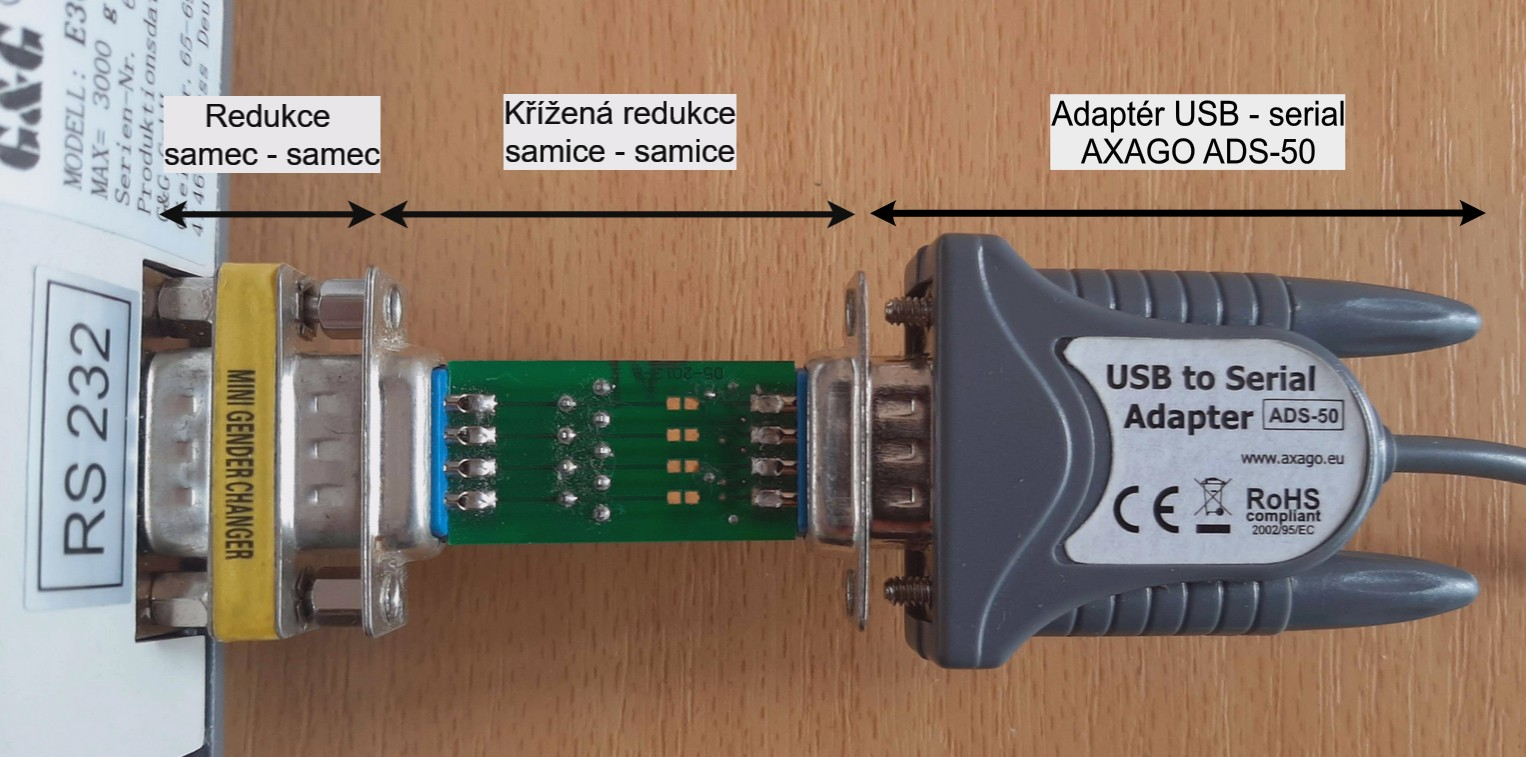
\includegraphics[scale=0.27]{obrazky/zapojení váhy.jpg}
    \end{center}
    \caption{Propojení váhy s mikropočítačem pomocí komponent dodané výrobcem váhy}
    \label{propojení váhy v1}
\end{figure}

\begin{figure}[H]
    \begin{center}
        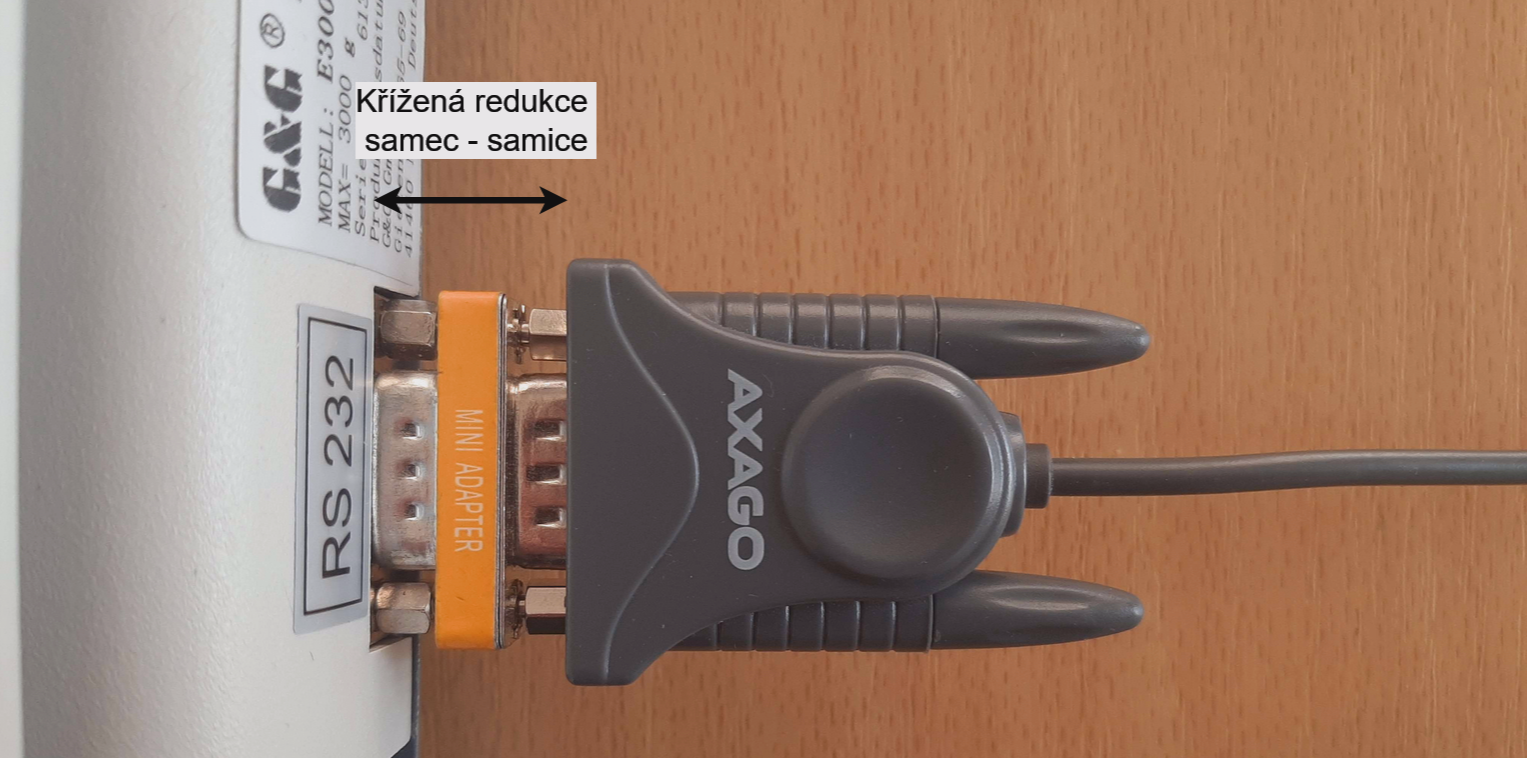
\includegraphics[scale=0.27]{obrazky/zapojeni_vahy_v2 - popis.png}
    \end{center}
    \caption{Výsledné propojení váhy s mikrokontrolerem}
    \label{propojení váhy v2}
\end{figure}

Dalším krokem je nastavení parametrů sériové komunikace podle manuálu váhy\cite{vaha_datasheed}. Komunikace byla testována pomocí osciloskopu s funkcí čtení UART protokolu a windows nástroje PuTTY, který přijímal/odesílal data po sériové lince. 
Na obrázku č. \ref{putty} je nastavení parametrů v PuTTY a na obrázku č.\ref{puttyyyy} je vidět, že váha nám na výstup konzole PuTTY posílá aktuální naměřená data.


\begin{figure}[H]
    \begin{center}
        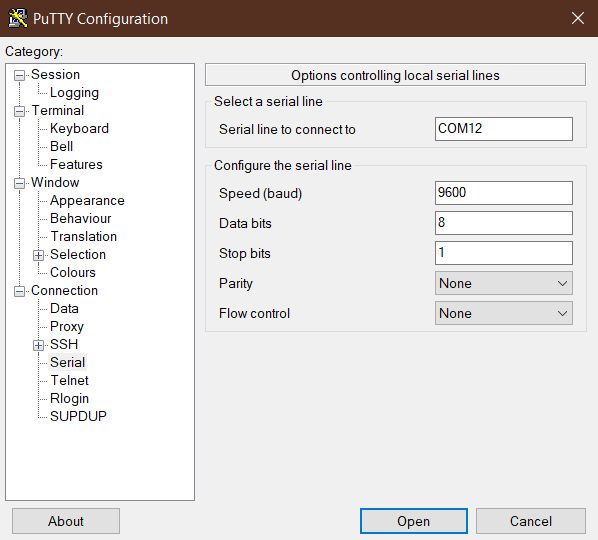
\includegraphics[scale=0.8]{obrazky/nastaveni putty.png}
    \end{center}
    \caption{Nastavení parametrů komunikace v PuTTY}
    \label{putty}
\end{figure}

\begin{figure}[H]
    \begin{center}
        %\includegraphics[scale=0.09]{obrazky/komunikace váha putty.jpg}
        \includegraphics[scale=0.12]{obrazky/komunikace váha putty - spodek.jpg}
        \includegraphics[scale=0.12]{obrazky/komunikace váha putty - vrch.jpg}
    \end{center}
    \caption{Čtení sériové komunikace váhy pomocí PuTTY}
    \label{puttyyyy}
\end{figure}

Na obrázku č.\ref{osc} byl datový výstup váhy testován pomocí osciloskopu. Parametry na osciloskopu byly nastaveny obdobně jak na obrázku č.\ref{putty}

\begin{figure}[H]
    \begin{center}
        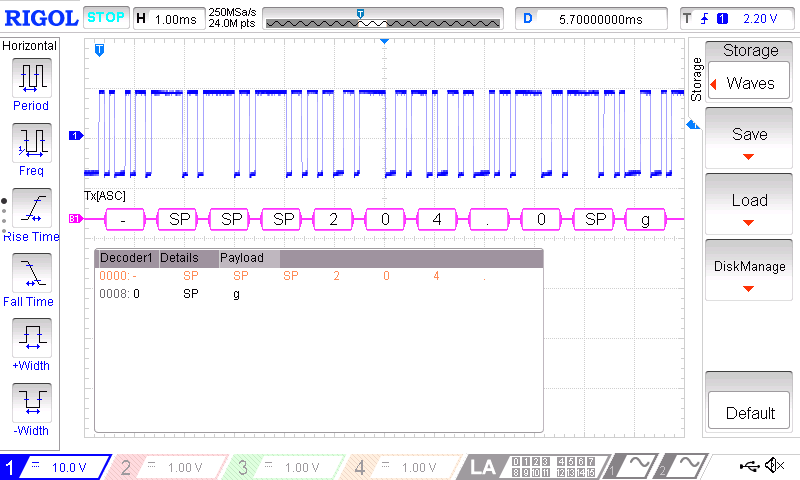
\includegraphics[scale=0.5]{obrazky/DS1Z_QuickPrint6.png}
    \end{center}
    \caption{Odchycení zprávy "-204.0 g" pomocí osciloskopu}
    \label{osc}
\end{figure}

%%%%%%%%%%%%%%%%%%%%%%%%%%%%%%%%%%%%%%%%%%%%%%%%%%%%%%%%%%%%%%%%%%%%%%%%%%%%%%%%%%%%%%%%%%%%%%%%%%%%%%%%%%%%%%%%%%%%%%%%%%%%%%%%
\section{Zprovoznění čtečky čárového kódu}
\label{zprovozeni_ctecky}
%Čtečka čárového kódu ve výchozím nastavení se chová jako klávesnice(HID KBW), aby bylo možné číst sériovou komunikaci je nutné naskenovat QR kód z manuálu\cite{scaner}, který přepíná výstup čtečky z HID KBW na virtuální sériový USB port(USB VCom).

Čtečka čárového kódu se ve výchozím nastavení chová jako klávesnice (USB HID KBW). To znamená, že pokud máme otevřený textový editor (například Word) a načteme čárový kód, data se vypíšou přímo do dokumentu, jako by byla zadána z běžné klávesnice.

Tento režim je však pro programové zpracování dat nepraktický – neumožňuje obousměrnou komunikaci, data nejsou strukturována do žádného rámce a není možné spolehlivě rozlišit začátek a konec zprávy. Výstup je navíc směrován do aktivního okna systému, což ztěžuje jeho přesné zachycení v aplikacích.

Z těchto důvodů výrobce poskytuje možnost přepnout čtečku do režimu USB VCOM (virtuální COM port). V tomto režimu čtečka emuluje sériový port přes USB, což umožňuje snadné a přesné čtení výstupu v programech jako je Python, HTerm nebo PuTTY – včetně možnosti odesílat příkazy zpět do čtečky.
\\\\
Čtečka tedy nabízí 3 komunikační rozhraní:
\begin{itemize}
    \item \textbf{UART} - Jeden z nejjednodušších sériových komunikačních protokolů, viz kapitola č. \ref{UART protokol}. Připojení k Raspberry Pi pomocí označených GPIO pinů: Tx a Rx. 
    \item \textbf{USB HID (Human Interface Device)}
    \begin{itemize}
        \item \textbf{USB HID KBW (Keyboard)} - emulace klávesnice (výchozí nastavení)
        \item \textbf{USB HID POS (Point of Sales)} - speciální protokol pro POS aplikace 
    \end{itemize}
    \item \textbf{USB VCom} - Virtuální sériový COM port, který emuluje UART komunikaci přes USB. Oproti klasickému UART rozhraní je USB VCOM stabilnější (integrovaná nízkoúrovňová CRC kontrola přenosu), jednodušší na zapojení a automaticky detekuje odpojení kabelu.
\end{itemize}
\bigskip
Po zapnutí se čtečka může nacházet ve třech různých provozních stavech, které jsou navrženy s ohledem na minimalizaci elektrické spotřeby:
\begin{itemize}
    \item \textbf{Operating (160 mA)} – Čtečka je aktivní a nachází se v režimu čtení. Je schopna okamžitě snímat a dekódovat čárové kódy.
    \item \textbf{Standby (30 mA)} – Čtečka se nachází v pohotovostním režimu, ve kterém čeká na aktivační impuls (např. detekce pohybu před senzorem, příkaz po sériové lince nebo stisk tlačítka). Po přijetí podnětu automaticky přechází do režimu čtení.
    \item \textbf{Sleep (3 mA)} – Nízkopříkonový režim, do kterého čtečka přechází po delší době nečinnosti. Funguje obdobně jako režim standby, avšak s výrazně nižší spotřebou energie. Nevýhodou je delší doba probuzení do režimu čtení (operating).
\end{itemize}
\bigskip
Čtečka čárového kódu má několik režimů čtení:
\begin{itemize}
    \item \textbf{Manuální (Manual)} - Pomocí fyzického tlačítka na těle čtečky.
    \item \textbf{Kontinuální (Continuous)} - Nepřetržité čtení.
    \item \textbf{Indukční (Induction)} - Čeká v standby režimu dokud nedetekuje změnu v obraze, pak se přepne do operating režimu.
    \item \textbf{Vyvolaný příkazem (Command Triggered)} - Čtečka začne skenovat po přijetí příkazu. Vhodné pro ovládání čtečku programem.
    \item \textbf{POS} - Přednastavený Command Triggered režim pro pokladní systémy - vypnutí oznamovacího zvuku při zapnutí čtečky, pakety posílány po sériové lince jsou bez ukončovacího znaku.
\end{itemize}
\bigskip
Funkčnost čtečky byla ověřena v režimu čtení \textit{Triggered} prostřednictvím rozhraní USB VCom za použití nástroje HTerm. Tento nástroj, na rozdíl od PuTTY, umožňuje odesílání dat ve formátu hexadecimálních řetězců, což je zásadní pro inicializaci čtečky do \textit{operating režimu} – stavu, ve kterém je schopna aktivně detekovat a dekódovat čárové kódy. Na základě technické dokumentace je pro spuštění skenovací sekvence nutné odeslat specifický příkaz ve formátu [\textbf{0x7E 0x00 0x08 0x01 0x00 0x02 0x01 0xAB 0xCD}], přičemž zařízení v případě úspěšného přijetí odpoví potvrzovací zprávou (tzv. ACK - \textit{acknowledgement code}) ve tvaru [\textbf{0x02 0x00 0x00 0x01 0x00 0x33 0x31}]. Výsledek této komunikace je zachycen na obrázku č. \ref{Zprovoznění čtečky}. Parametry pro sériovou komunikaci byly nastaveny stejně jak u váhy[\ref{putty}].

\section{Integrace čtečky do řídicí logiky systému}
% ME: Implementace čtečky do stavového automatu / Ovládání / Obsluha čtečky / Výběr čtecího režimu
% AI: Integrace čtečky do řídicí logiky systému / Řízení čtečky pomocí stavového automatu / Výběr čtecího režimu pro řízené snímání
Čtečka bude řízena programově prostřednictvím stavového automatu a aktivována pouze v okamžiku, kdy je potřeba provést identifikaci alkoholu (např. načtením EAN kódu nebo ručním výběrem produktu). Naskenování čárového kódu bude doprovázeno zvukovou a optickou signalizací – prostřednictvím integrované LED diody a bzučáku, které automaticky reagují při úspěšném přečtení kódu. LED dioda zároveň slouží k nasvícení kódu v podmínkách se zhoršenou viditelností.

V rámci návrhu stavového automatu je nutné čtečku z pohledu uživatele „zapínat“ (Operating režim) a „vypínat“ (Standby režim), aby nedocházelo k nechtěnému čtení a tím i chybné signalizaci nebo přenosu dat. V běžném provozu bohužel čtečku nelze explicitně přepnout příkazem do Standby režimu. Například v režimu Triggered přejde čtečka do Standby buď po úspěšném načtení kódu, nebo po uplynutí definovaného časového intervalu (0.1 – 25 s). Pokud však uživatel kód neoskenuje (např. zvolí produkt ručně), čtečka zůstane v aktivním režimu a je možné omylem načíst další kódy i mimo určený stav automatu.

Jelikož přechod mezi režimy nelze ovládat přímo příkazem, jedinou možností řízení ze strany programu bez nutnosti restartu čtečky zůstává zapínání/vypínání LED a bzučáku. Níže jsou uvedeny možné varianty, jak se s tímto omezením vyrovnat:

\begin{itemize}
    \item \textbf{Přerušení napájení} - Pomocí externího spínacího obvodu (např. tranzistoru řízeného přes GPIO), který by odpojil napájení čtečky nebo čtečku napájet přímo GPIO pinem, který by se spínal - Tento přístup by neumožňoval připojení přes USB a vyžadoval by komunikaci přes rozhraní UART.
    \item \textbf{Vymazání vstupního bufferu} - Čtečka sice nejde explicitně přepnout do Standby režimu, ale lze ji ponechat aktivní s vypnout LED a zvukovou signalizací. Z pohledu uživatele čtečka působí jako neaktivní, protože neposkytuje žádnou zpětnou vazbu, i když stále čte. Pokud dojde k náhodnému načtení kódu mimo požadovaný stav, příslušná data se uloží do vstupního bufferu mikrokontroléru, který lze následně programově vyprázdnit. Tento přístup lze využít například v režimu Continuous, kdy čtečka zůstává trvale aktivní.
    \item \textbf{Periodické spouštení čtečky} - V Triggered režimu nastavit krátký interval čtení a periodicky odesílat příkaz ke spuštění čtečky (Operating režim). Tato metoda není nejvhodnější z hlediska časové a výpočetní náročnosti – program je neustále přerušován odesíláním příkazů v krátkých intervalech a čekáním na ACK.
    \item \textbf{Přepínání do manuálního režimu} (aktuální řešení): V Manual režimu čtečka čeká v standby stavu dokud uživatel nezmáčkne tlačítko, tohle tlačítko ve finální verzi měřícího systému nebude fyzicky přístupné (čtečka bude schovaná v krabičce). Čtečka na základě stavového automatu bude přepínána mezi Countiual a Manual režimem.
\end{itemize}




\begin{figure}[h]
    \begin{center}
        \includegraphics[scale=0.14]{obrazky/hterm_ctecka_oriznutí.png}
    \end{center}
    \caption{Čtení sériové komunikace čtečky pomocí HTerm}
    \label{Zprovoznění čtečky}
\end{figure}

%Čtečku bude spuštěna jen v určitém stavu programu, proto využijeme trigger mode, který nám zajístí, že uživatel nenačte čárový kod kdy nemá. To může způsobit hromadění kodu v bufferu mikrokontroleru/řídící jednotky
\\\\
%Čtečku čárového kódu lze připojit pomocí UART nebo USB rozhraní.

%Zjistit v jakem formatu mi to posílá

%%%%%%%%%%%%%%%%%%%%%%%%%%%%%%%%%%%%%%%%%%%%%%%%%%%%%%%%%%%%%%%%%%%%%%%%%%%%%%%%%%%%%%%%%%%%%%%%%%%%%%%%%%%%%%%%%%%%%%%%%%%%%%%%
\section{Zprovoznění dotykového displeje}
%Vybraný dotykový displej JOY-IT, má rozlišení 1024 x 600 px s poměrem stran 128:75, což přibližně odpovídá poměru 17:10. Raspberry Pi OS vybírá rozlišení podle seznamu podporovaných rozlišení CEA (Consumer Electronics Association) a DMT (Display Monitor Timings), které jsou standardní a široce kompatibilní s většinou monitorů a televizí. Rozlišení vybraného displeje nespadá do žádné zmíněné kategorie a je nutné jej nastavit ručně prostřednictvím systémového souboru 'config.txt' .[z1][z2] Pokud by rozlišení displeje se neshodovalo s rozlišením obrazovky, tak by se obraz musel škálovat (upraven tak, aby se vešel na fyzický rozměr displeje, což znamená jeho zvětšení nebo zmenšení), což by vedlo ke snížení kvality obrazu, dále pokud by rozlišení obrazovky překročilo rozlišení displeje, tak by došlo k většímu vytížení GPU.

Vybraný dotykový displej JOY-IT má rozlišení 1024×600 px a poměr stran 128:75, což přibližně odpovídá poměru 17:10. Systém Raspberry Pi OS automaticky volí rozlišení z nabídky standardizovaných režimů CEA (Consumer Electronics Association) a DMT (Display Monitor Timings), které jsou široce kompatibilní s většinou monitorů a televizorů. Rozlišení vybraného displeje nespadá do žádné zmíněné kategorie a je nutné jej nastavit ručně úpravou systémového souboru config.txt, konfiguračního souboru 10-monitor.conf. nebo využít utilit pro nastavení obrazu displeje, např. Xrandr.[z1][z2]
Pokud by se skutečné rozlišení displeje neshodovalo s nastaveným rozlišením obrazovky, byl by obraz škálován (zvětšen nebo zmenšen na fyzickou velikost displeje), což by zhoršilo jeho kvalitu. V případě, že by rozlišení obrazovky překročilo nativní rozlišení displeje, došlo by současně k větší zátěži GPU.

\subsection{Nastavení rozlišení obrazovky pomocí utility Xrandr}
%Použijem příkaz "cvt" (Coordinated Video Timing), který pro zvolené rozlišení vypíše informaci, jako je obnovovací frekvence, horizontální frekvence synchronizace (hsync) a pixel clock (pclk). Tyto informace jsou nutné pro nastavení nového rozlišení pomocí Xrandr.
%Pro nastavení nového rozlišení využívám příkaz "cvt" (Coordinated Video Timing), který poskytuje podrobné informace o zvoleném rozlišení, včetně obnovovací frekvence, horizontální frekvence synchronizace (hsync) a pixel clock (pclk). Tyto údaje jsou nezbytné pro konfiguraci nového rozlišení pomocí nástroje Xrandr.

Pro nastavení nového rozlišení (1024×600 px) využívám nástroj Xrandr, který vyžaduje znalost konkrétních časovacích parametrů – obnovovací frekvence, horizontální frekvence synchronizace (hsync) a pixel clocku (pclk). Tyto hodnoty získám z příkazu cvt (Coordinated Video Timing), který je dopočítá na základě požadovaného rozlišení.

%Pro konfiguraci nového rozlišení jsem  nového rozlišení využil jsem
%Pro konfiguraci rozlišení v linuxovém prostředí exituje více druhů nástrojů, já jsem si zvolil Xrandr, který vyžaduje výše zmíněné informace z příkazu "cvt"

%language = bash nebo sh
%%%%%%%%%%%%%%%%%%%%%%%%%%%%%%%%%%%%%%%%%%%%%%%%%%%%%%%%%%%%%%%%%
\captionsetup[lstlisting]{labelformat=empty}
\lstdefinelanguage{bashcolored}{
  language=bash,
  basicstyle=\ttfamily\small,
  commentstyle=\color{gray},
  keywordstyle=\color{blue},
  moredelim=**[is][\color{gray}]{@}{@}, % výstup obarvíš pomocí @...@
}
\begin{lstlisting}[language=bashcolored, caption=Příklad použití příkazu cvt (Linux terminál):, frame=single, breaklines=true, postbreak=\mbox{\textcolor{gray}{$\hookrightarrow$}\space}]
$cvt 1024 600
# 1024x600 59.85 Hz (CVT) hsync: 37.35 kHz; pclk: 49.00 MHzxa
@Modeline "1024x600\_60.00"   49.00  1024 1072 1168 ... [1]@

\end{lstlisting}
%\footnotemark
\footnotetext[1]{Plné znění odpovědi: \texttt{Modeline "1024x600\_60.00"   49.00  1024 1072 1168 1312  600 603 613 624 -hsync +vsync}}

\begin{lstlisting}[language=bash, caption=Na základě nově vygenerovaných parametrů vytvoříme nový režim pomocí Xrandr:, frame=single]
$xrandr --newmode  "1024x600\_60.00" 49.00 1024 ... [2]
\end{lstlisting}
\footnotetext[2]{Plné znění příkazu: \texttt{\$xrandr --newmode  "1024x600\_60.00"   49.00  1024 1072 1168 1312  600 603 613 624 -hsync +vsync}}

\begin{lstlisting}[language=bash, caption=Nově vytvořený režim přiřadíme k požadovanému video výstupu (např. HDMI-1):, frame=single]
$xrandr --addmode HDMI-1 "1024x600\_60.00"
\end{lstlisting}

\begin{lstlisting}[language=bash, caption=Nyní změníme rozlišení obrazovky:, frame=single]
$xrandr --output HDMI-1 --mode "1024x600\_60.00"
\end{lstlisting}
\captionsetup[lstlisting]{labelformat=default}
%%%%%%%%%%%%%%%%%%%%%%%%%%%%%%%%%%%%%%%%%%%%%%%%%%%%%%%%%%%







%%%%%%%%%%%%%%%%%%%%%%%%%%%%%%%%%%%%%%%%%%%%%%%%%%%%%%%%%%%%%
%Příklad použití příkazu cvt (terminál Linuxu):
%
%\$ cvt 1024 600
%
%\# 1024x600 59.85 Hz (CVT) hsync: 37.35 kHz; pclk: 49.00 MHzxa
%Modeline "1024x600\_60.00"   49.00  1024 1072 1168 1312  600 603 613 624 -hsync +vsync
%\\
%\\
%Následně vytvoříme nový režim pomocí Xrandr:
%
%\$xrandr --newmode  "1024x600\_60.00"   49.00  1024 1072 1168 1312  600 603 613 624 -hsync +vsync
%\\
%\\
%Nově vytvořený režim přidáme k požadovanému video výstupu (HDMI-1):
%
%\$xrandr --addmode HDMI-1 "1024x600\_60.00"
%\\
%\\
%Nyní změníme rozlišení obrazovky pomocí:
%
%\$xrandr --output HDMI-1 --mode "1024x600\_60.00"
%\\
%\\
%%%%%%%%%%%%%%%%%%%%%%%%%%%%%%%%%%%%%%%%%%%%%%%%%%%%%%%%%%%%%%
%Toto nastavení se neukládá a pokud chceme mít nově nastavené rozlišení i po opětovném spuštění raspberry pi je nutné jej uložit do souboru, který se spouští současně se systémem jako např. /etc/X11/xorg.conf.d/10-monitor.conf

%Toto nastavení není trvalé a aby zvolené rozlišení zůstalo zachováno i po opětovném spuštění Raspberry Pi, je třeba jej uložit do konfiguračního souboru, například \textbf{/etc/X11/xorg.conf.d/10-monitor.conf.}




%Nastavení rozlišení obrazovky pomocí systé

%V případě zvětšení(upscaling) by obraz ztrácel na přesnosti a byl by rozmazaný, zatím co při zmenšení(downscaling) by obraz ztrácel na detailech

%z1: raspbery dokumentace - co je v zadání BP
%z2: https://elinux.org/RPiconfig#Camera

%\newcounter{keepage}
%\setcounter{keepage}{\value{page}} % uložíme aktuální číslo
%\pagenumbering{gobble}
%
%
%\clearpage
%\pagenumbering{arabic}
%\setcounter{page}{\value{keepage}} % vrátíme 28
%\addtocounter{page}{}             % posuneme na 29

%%%%%%%%%%%%%%%%%%%%%%%%%%%%%%%%%%%%%%%%%%%%%%%%%%%%%%%
%%%%%%%%%%%%%%%%%%%%%%%%%%%%%%%%%%%%%%%%%%%%%%%%%%%%%%%
%%%%%%%%%%%%%%%%%%%%%%%%%%%%%%%%%%%%%%%%%%%%%%%%%%%%%%%

\chapter{Vývoj firmware a zprovoznění systému jako celku}
%\addcontentsline{toc}{chapter}{Vývoj firmware a zprovoznění systému jako celek}

V této kapitole se budu zabývat návrhem firmwaru s grafickým rozhraním pro mikropočítač Raspberry Pi 4, výběrem programovacího jazyka a ošetřením nežádoucích
stavů. Kapitola je rozdělená do dvou částí, jedna se zabývá čistě vizuální stránkou a interakcí mezi jednotlivými okny firmwaru a druhá část se zabývá čistě programovým řešením a komunikací mezi jednotlivými soubory firmwaru. Výsledný systém se mírně liší od původního konceptu na základě jeho testování v praxi a postupného vylepšování.
Většina kódu bude prezentována jen hlavičkou metod, funkcí a tříd z důvodu rozsáhlého obsahu.

%-----
\section{Výběr programovacího jazyka a grafické knihovny}
Jako programovací jazyk jsem zvolil Python na základě jednoduché syntaxe a čitelnosti kódu. Python má rozsáhlé množství knihoven pro vývoj GUI aplikací a je také velmi populární v komunitě \textit{Raspberry Pi}, což přináší spoustu dostupných zdrojů a podpory.

Grafická knihovna byla vybrána \textit{Tkinter} na základě rozsáhlé dokumentace, jednoduchosti na naučení, velkého množství ovládacích prvků (widgetů), ale hlavně licence PSFL, která dovoluje libovolné (vč. komerční) využití při zachování copyrightu a textu licence bez jakýchkoliv finančních nákladů. [z1]
%https://docs.python.org/3/license.html

%-----
\section{Rozložení zdrojových souborů a jejich vzájemná vazba}

Celý program se skládá z 5 souborů obsahujících zdrojový kód v jazyce Python s příponou .py.

\begin{itemize}
    \item \textbf{main.py} - Obsahuje stavový automat, který se opakovaně volán, díky hlavní smyčce, kterou vytváři  mnou vytvořená grafická třída gui.py, která dále dědí z grafického modulu Tkinter.py. Tato problematika je podrobněji rozebrána v samotné sekci gui.
    \item \textbf{gui.py} - Obsahuje veškerý kód týkající se grafického vykreslení.
    \item \textbf{barcode\_sensor.py} - zastřešuje veškerou komunikaci se čtečkou.
    \item \textbf{scale.py} - Zastřešuje veškerou komunikace s váhou.
    \item \textbf{database.py} - Zastřešuje veškerou komunikaci s databázi.
\end{itemize}


%-----
\section{Konečný stavový automat}
Aby nám celý systém mohl fungovat, musí se řídit nějakou logikou a posloupností jednotlivých stavů, proto byl navržený stavový automat dle kterého je vytvořený celý program firmwaru. Tento stavový automat je reprezentovaný jako funkce opakovaně volající se funkce v hlavním souboru programu - main.py

\begin{figure}[H]
    \begin{center}
        \includegraphics[scale=0.4]{obrazky/stavový automat_2.jpg}
    \end{center}
    \caption{Interakce mezi okny GUI}
    \label{Interakce mezi okny GUI}
\end{figure}
//OBRÁZEK - Stavového automatu z pohledu uživatele

Z pohledu programu, ale stavový automat vypadá trochu jinak, protože některé stavy jsou zaobalené do do jedné funkce programu, abysme nevytvářeli zbytečně mnoho funkcí kvůli vykonání jednoho příkazu (jeden řádek kódu). Níže je zobrazen stavový diagram z pohledu programu.

//OBRÁZEK - Stavového automatu z pohledu programu

\subsection{Zdrojový soubor konečného stavového automatu - main.py}
%V hlavním souboru je zadefinováná třída \texttt{Automat}, která dědí ze třídy \texttt{Enum} pro vytvoření jednotlivých stavů automatu. Využití konstant nesoucí název daného stavu činí kód přehlednější než použití běžných číselných konstant.

V hlavním souboru je zadefinováná třída \texttt{Automat}, která dědí ze třídy \texttt{Enum}, která umožňuje vytvoření jednotlivých stavů automatu jako konstanty nesoucí jejich název. Instance této třídy pak bude vždy rovná hodnotě, ve které se zrovna nachází stavový automat.

%\begin{lstlisting}[language=Python, caption=Hlavní okno, frame=single]
%from enum import Enum
%
%class Automat(Enum):
%    STARTING_INVENTORY = 0
%    CHECK_PORT = 1
%    FINDING_DISTILLATE = 3
%    SAME_DISDILLATE = 4
%    WEIGHING = 5
%    REMOVE_BOTTLE = 6
%\end{lstlisting}

%Třída Automat je následně využita ve funkci state\_machine obsahující rozhodovací blok pomocí zřetězených podmínek if/elif. Funkci předáváme počáteční stav automatu tedy STARTING\_INVENTORY. Některé funkce stavového automatu mají incializační podmínku, která se vykoná pouze jednou při vstupu do nového stavu. Globální proměnná state\_pre si pamatuje předchozí stav automatu a pokud se nerovná aktuálnímu stavu, tak se globální proměnná set\_up nastaví na true, což způsobí povolení inicializační podmínky.

%Některé funkce stavového automatu mají incializační podmínku, která se vykoná pouze jednou při vstupu do nového stavu, k povolení této podmínky slouží globální proměnná set\_up, která se nastaví na True v případě, že globální proměnná state\_pre, která uchovává předchozí stav automatu, se nerovná aktuálnímu stavu automatu.

%Třída Automat je v kódu využita ve funkci state_machine, která pracuje s rozhodovacím blokem pomocí zřetězených podmínek if/elif. Této funkci se předává počáteční stav automatu, tedy STARTING_INVENTORY. Některé funkce stavového automatu obsahují inicializační podmínku, která se vykoná pouze jednou při vstupu do nového stavu. K jejímu povolení slouží globální proměnná set_up, jež se nastaví na True v případě, že globální proměnná state_pre (uchovávající předchozí stav automatu) se nerovná aktuálnímu stavu. Pokud se tedy state_pre liší od nového stavu, set_up se nastaví na True a dojde k provedení kódu, který se má spustit jen při přechodu do stavu.

%V prezentovaném kódu stavového automatu se využívá třída Automat, jejíž hodnoty reprezentují jednotlivé stavy. Funkce state_machine využívá zřetězených podmínek if/elif pro rozhodování, který stav se má vykonat – výchozím je STARTING_INVENTORY. Při vstupu do každého nového stavu může nastat situace, kdy se provádí jednorázový inicializační kód (tzv. setup). K jeho spuštění slouží globální proměnná set_up, která se nastaví na True jen tehdy, když detekujeme přechod do nového stavu. To zajišťuje kontrola nad globální proměnnou state_pre: pokud se liší od aktuálního stavu, znamená to změnu a set_up se nastaví na True. Tím se umožní vykonání inicializačních kroků pouze jednou v okamžiku vstupu do daného stavu.

%Třída Automat je využívána ve funkci state_machine, která implementuje stavový automat pomocí rozhodovacího bloku složeného ze zřetězených podmínek if/elif. Této funkci je při volání předán počáteční stav automatu, tedy STARTING_INVENTORY. Některé funkce jednotlivých stavů obsahují inicializační část, která se provede pouze jednou při vstupu do nového stavu. K řízení této inicializace slouží globální proměnná set_up, která se nastaví na hodnotu True, pokud se předchozí stav automatu uložený v globální proměnné state_pre liší od aktuálního stavu. Tímto způsobem je zajištěno, že inicializační část daného stavu je vykonána vždy právě jednou.

Třída \texttt{Automat} je využívána ve funkci \texttt{state\_machine}, která implementuje stavový automat pomocí rozhodovacího bloku složeného ze zřetězených podmínek \texttt{if/elif}, které určují, který stav se má vykonat. Při prvním volání funkce se jí předá počáteční stav \texttt{STARTING\_INVENTORY}. 

Některé funkce jednotlivých stavů obsahují inicializační podmínku, která se provede pouze jednou při vstupu do nového stavu. K řízení této inicializace slouží globální proměnná \texttt{set\_up}, která se nastaví na hodnotu \texttt{True}, pokud se předchozí stav automatu uložený v globální proměnné \texttt{state\_pre} liší od aktuálního stavu. Tímto způsobem je zajištěno, že inicializační část daného stavu je vykonána vždy právě jednou.



%U poslední podmínky, předáváme funkci "stop\_inventory" aktuální stav automatu, protože tato funkce může být volána z vicero stavech a taky se vrátit do stavu z kama byla volána dle obrázku stavového diagramu a při možnosti vrácení se zpět je nutné si uchovat informaci o posledním stavu, aby se vrátila do toho původního

%U poslední podmínky, předáváme funkci "stop\_inventory" aktuální stav automatu. Dle stavového diagramu můžeme ukončit inventuru z víceromíst, případně z ukončovacího stavu se vrátit do předchozího a abych se do tohoto stavu mohli vrátit je nutné si uchovat informace o stavu z kterého jsme přešli. V praxi to znamená, že zavřeme ukončovací obrazovku a to nás vrátí do předchozího stavu.

U poslední podmínky je funkci \texttt{stop\_inventory} předáván aktuální stav automatu. Podle stavového diagramu je možné ukončit inventuru z více částí aplikace a případně se z ukončovacího stavu vrátit zpět do stavu předchozího. Aby byl návrat do původního stavu uskutečnitelný, je nezbytné uchovat informaci o tom, odkud byl přechod proveden. V praxi to znamená, že při zavření ukončovací obrazovky dojde k návratu do stavu, ve kterém se aplikace nacházela před přechodem do ukončovací fáze.

%Metoda app.after() patří grafické třídě, více rozebráno v sekci xx, která spouští hlavní smyčku programu, kde po každých 20 ms volá metodu after. Tato třída spouští hlavní smyčku programu, obstarávající chod GUI, aby bylo možné z této smyčky vyskočit je využívána metoda after, kde její 1. argumentem je časový interval, za jak dlouho se tato funkce zavolá po spuštění hlavní smyčky a 2. argumentem je funkce state\_machine kterou bude volat, tzv. zpětné volání (callback function), dalším parametrem je *args, který reprezentuje libovolný počet parametrů libovolného datového typu, které budou předány jako parametr funkce z 2. argumentu funkce, tedy se zavolá funkce statemachine a předá se ji parametr state - Toto zapříčiní u funkce state\_machine opakované volání sebe sama, každých 20 ms.

%1. argument je časový interval za jak dlouho se zavolá funkce, která je 2. argumentem, které se předá parametr, který je 3. argumentem, tedy metoda after zavolá každých 20 ms funkci state machine a předá ji parametr state.

%Metoda app.after(20, state\_machine, state) patří grafické třídě viz sekce č.[bude doplněno]. Tato třída spouští hlavní smyčku programu, obstarávající chod GUI a aby bylo možné z ní vyskočit využívá se zmíněné metody, která konrétně v našem případě volá funkci state\_machine (druhý parametr metody), jedná se o tzv. zpětné volání (callback function) a předává ji parametr state (třetí parametr metody). Metoda se vykoná pouze jednou po spuštění hlavní smyčky, proto je opakovaně volána každých 20 ms(první parametr metody) na konci funkce.

%Metoda app.after(20, state_machine, state) je součástí grafické třídy (viz sekce č. [bude doplněno]). Tato třída spouští hlavní smyčku programu, která zajišťuje chod uživatelského rozhraní (GUI). Aby bylo možné tuto smyčku v případě potřeby ukončit, využívá se právě uvedená metoda, která v daném případě volá funkci state_machine (druhý parametr) formou zpětného volání (callback function) a předává jí parametr state (třetí parametr). Vzhledem k tomu, že se metoda po spuštění hlavní smyčky provede pouze jednou, je na konci funkce naplánováno její opakované volání každých 20 ms (hodnota prvního parametru). Tím je zajištěn pravidelný cyklus, v němž se state_machine vykonává a zároveň je GUI průběžně aktualizováno.

%Metoda app.after(20, state\_machine, state) je součástí grafické třídy GUI (viz sekce č. [bude doplněno]). Tato třída spouští hlavní smyčku programu, která zajišťuje chod uživatelského rozhraní (GUI). Aby bylo možné z této smyčky v případě potřeby vyskočit, využívá se právě uvedená metoda, která v daném případě volá funkci state\_machine (druhý parametr) formou zpětného volání (callback function) a předává jí parametr state (třetí parametr). Vzhledem k tomu, že se metoda po spuštění hlavní smyčky provede pouze jednou, je na konci funkce naplánováno její opakované volání každých 20 ms (první parametr). Tím je zajištěn pravidelný cyklus, v němž se state\_machine vykonává a zároveň je GUI průběžně aktualizováno.

%Aby bylo možné opakovaně volat funkci state machine je nutné z této smyčky vyskočit 

Metoda \texttt{app.after(20, state\_machine, state)} je součástí grafické třídy \texttt{GUI} (viz sekce č. [bude doplněno]), která opakovaně volá funkci \texttt{state\_machine} (druhý parametr) formou zpětného volání (callback function) každých 20 ms (první parametr) a předává jí parametr \texttt{state} (třetí parametr).


%, protože tato funkce může být volána z vicero stavech a taky se vrátit do stavu z kama byla volána dle obrázku stavového diagramu a při možnosti vrácení se zpět je nutné si uchovat informaci o posledním stavu, aby se vrátila do toho původního

%Tyto stavy dále jsou využitý ve funkci state\_machine, kde na základě aktuálního stavu předé jako aurgument funkce se vykoná příslušný stav

%Na základě stavu (proměná state). Mnou využitá verze pythonu nepodporuje switch case funkci, tudíž 

%Aktuální verze Pythonu (3.9.21) nepodporuje žádný příkaz podobný "switch", jak je známo z jiných programovacách jazycích, tudíž logika pro volání jednotlivých stavů automatu je pomocí podmínek "if".

\begin{lstlisting}[language=Python, caption=Funkce stavového automatu, frame=single, breaklines=true, postbreak=\mbox{\textcolor{gray}{$\hookrightarrow$}\space}]
state_pre: Automat = Automat.STARTING_INVENTORY
set_up: bool = True

def state_machine(state: Automat) -> None:
    global state_pre
    global set_up
    
    #switch statement by "if" condition (Python v 3.9.2)
    if state == Automat.STARTING_INVENTORY:
        state = starting_inventory()
                    ...
    elif state == Automat.REMOVE_BOTTLE:
        state = remove_bottle()

    if state_pre == state:
        set_up = False
    else:
        set_up = True
    state_pre = state
    
    if state != Automat.STARTING_INVENTORY and state != Automat.WEIGHING and app.button_stop_pressed:
        state = stop_inventory(state)

    app.after(20, state_machine, state)
\end{lstlisting}



//KOD

%-----
\section{Stav - Začátek inventury}
Při spuštění firmwaru se prvně zobrazí úvodní okno, díky kterému jsme schopni spustit samotnou inventuru. Je zde pouze viditelné tlačítko start a nastavení. Tlačítko strat jednoduše spustí celý systém a kdy je možné započít inventuru. Tlačítko nastavení na uvodni obrazovce je zdůvodu, pokud uživatel se chce podívat nebo nastavit aplikaci bez toho, aby musel spouštět inventuru, tato část je vice rozberáno v sekci [x]

%Toto okno je realizováno pomocí třídy Start_Window

%\begin{figure}[!h]
%    \begin{center}
%        
\includegraphics[scale=0.4]{obrazky/GUI Spuštění inventury.png}
%    \end{center}
%    \caption{Úvodní okno aplikace}
%    \label{Interakce mezi okny GUI}
%\end{figure}

\section{Stav - Ověření komunikace}
Po spuštění celého systému provedu ověření zda komunikuje čtečka a váha, to udělám pomocí funkce 
xx 
xx 

V případě uspěšné inicializace seriové komunikace funkce vráti True v opačném případě False. Toto chybové hlášení nám aplikace zobrazí v Proces labelu v hlavním okně aplikace (Hlavní okno je rozebráno o stav níže). Tyto metody spadají pod vytvořenou třídy Senzor a Scale, které jsou více rozebrýny v sekci č.x a č.y. 

\section{Stav - Vyhledání produktu}

Za předpokladu, že v předchozím stavu nedošlo k chybě se zde uživatel poprvé setkává s hlavním oknem aplikace v kterém je schopen vyhledat konkrétní produkt na základě naskenování jeho EAN kódu nebo ručního vyhledání pomocí klávesnice.

\subsection{Hlavní okno}
Hlavní okno jsem navrhoval s myšlenkou, aby uživatel mohl většinu interakcí vykonávat z jednoho místa bez nutnosti přepínání mezi více okny, čímž jsem chtěl ulehčit orientaci a rychlost práce s grafickým prostředím. Hlavní stránka ovšem mění své rozložení komponent s každým stavem nebo využitím pomocných tlačítek, ale celková struktura okna zůstává stejná. Tyto jednotlivé změny jsou rozebrány zvlášť v jednotlivých stavech automatu.

%V některých stavech nejsou přístupné některé ovládací prvky(tlačítka, text boxy, scrollovací lišta), v oblasti vývoje GUI se často používá anglický název widgety. Pokud ovládací prvek není dostupný pro daný stav, tak je zašedlý.

V některých stavech mohou být určité ovládací prvky (jako tlačítka, textová pole nebo posuvníky – tzv. widgety) nedostupné. Tyto prvky jsou v takovém případě vizuálně označeny jako neaktivní (zašedlé).

\begin{figure}[!h]
    \begin{center}
        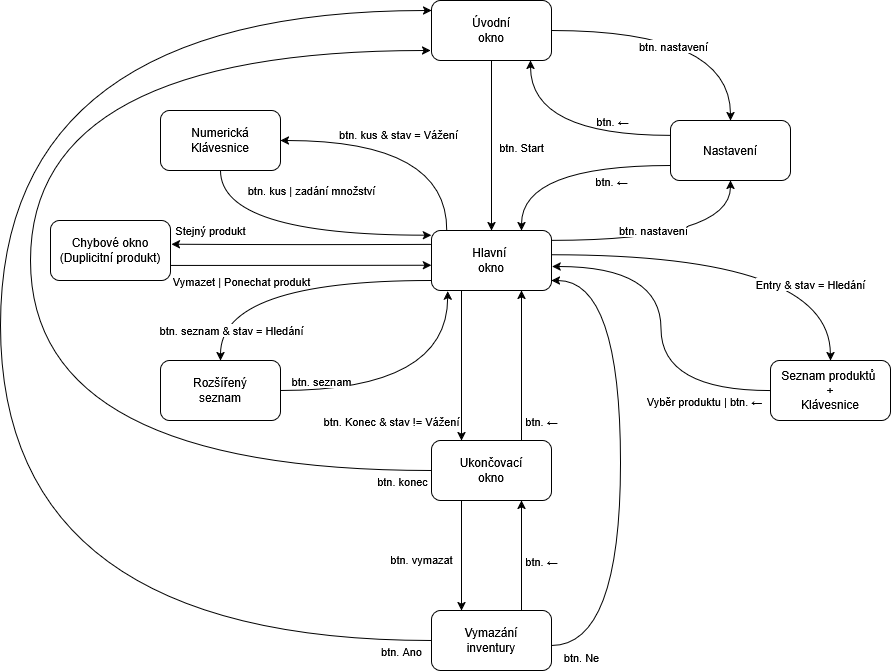
\includegraphics[scale=0.5]{obrazky/Interakce napříč okny GUI.png}
    \end{center}
    \caption{Interakce mezi okny GUI}
    \label{Interakce mezi okny GUI}
\end{figure}

\begin{figure}[H]
    \begin{center}
        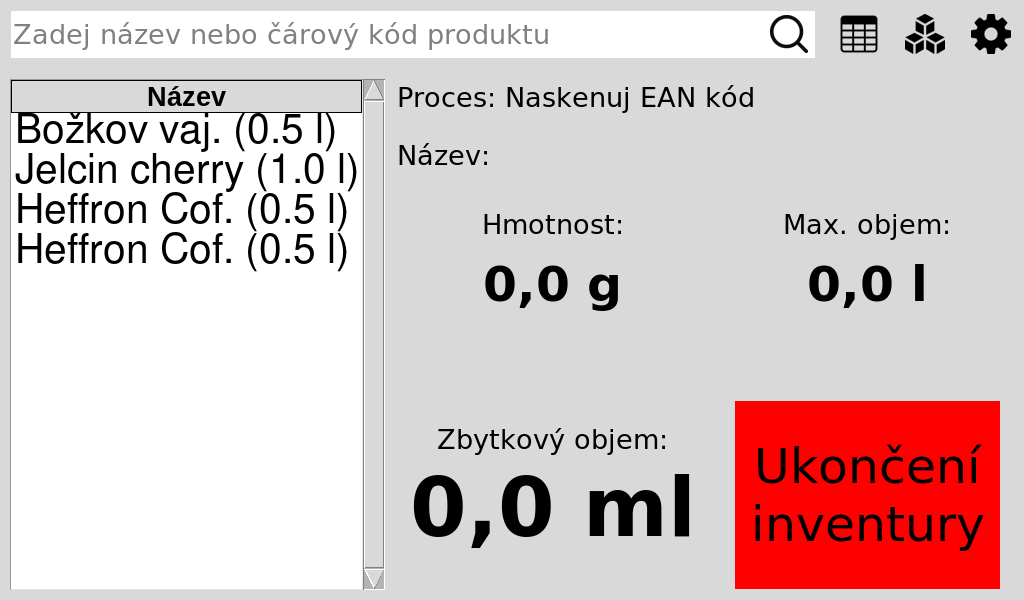
\includegraphics[scale=0.4]{obrazky/GUI Vyhledávání.png}
    \end{center}
    \caption{Hlavní okno ve stavu vyhledávání}
    \label{Interakce mezi okny GUI}
\end{figure}


//OBRAZEK - HL. MENU S PRVKY VE ZKRACENEM SEZNAMU
//Obrázek - komunikace mezi komponentami

\subsection{Proces vyhledání}

%Jak bylo řečeno vyhledání produktu probíhá naskenováním jeho EAN kódu. V přípdě neuspěšného scanu z důvodu poškozeného čárového kódu nebo že daný čárový kód není veden v databázi, systém vypíše do "label_proces" chybové hláčení "[bude doplěno]". V případě, že by byl čárový kód tak moc poškozen, že by nešel přečíst je možnost ho vyhledat ručně pomocí Entry pole. Po kliknutí na Entry pole vyjede seznam (list box) destilátů a ze spodní části obrazovky vyjede klávesnice pro rychlejší vyhledání pomocí zadání názvu.

%nebo ručním vyhledáním pomocí entry(text boxu), kdy po kliknutí na něj nám vyjede seznam se všemi produkty a ve spodní části obrazovky se ukáže klávesnice pro vyhledání

%V tomto stavu jsme schopni už vyhledávat požadovaný produkt buď naskenováním jeho EAN kodu nebo jeho ručním vyhledáním. Pokud se rozhodneme vyhledat produkt pomocí naskenování jeho kodu, ale ten se nepovede najít  případě, že by se nepovedlo vyhledat EAN kod, tak nas aplikace upozorní přes Proces label, že došlo k chybě. V případě ručního vyhledání využijeme Entry(textové pole), kdy na něj stačí kliknout a současně nám vyjede i klávesnice.

Vyhledávání produktu probíhá primárně naskenováním jeho EAN kódu. Pokud je kód nečitelný nebo v databázi neexistuje, zobrazí se chybová hláška [sdsd] v prvku label\_proces. V případě, že je kód natolik poškozený, že jej nelze načíst, je možné produkt dohledat ručně. Kliknutím do vstupního pole (Entry) se zobrazí seznam dostupných destilátů a zároveň se ve spodní části obrazovky otevře klávesnice pro rychlé zadání názvu.

\begin{figure}[H]
    \begin{center}
        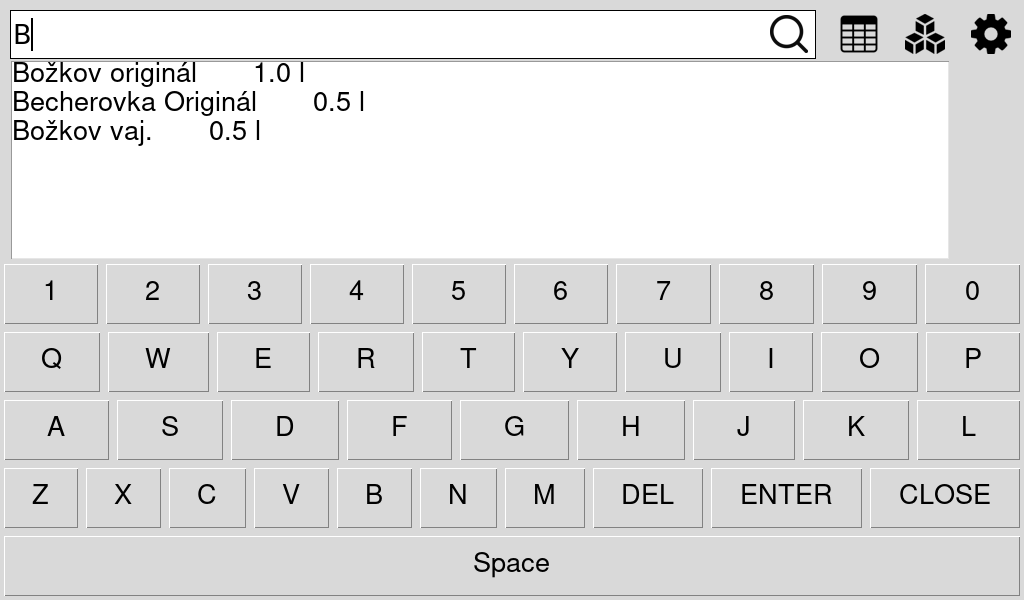
\includegraphics[scale=0.4]{obrazky/GUI Klavesnice + list_box + filr.png}
    \end{center}
    \caption{Hlavní okno - manuální vyhledání produktu}
    \label{Hlavní okno - manuální vyhledání produktu}
\end{figure}
//OBRÁZEK - JAK VYPADÁ RUČNÍ VYHLEDÁNÍ = LISTBOX + KBW

%Do prvku canvas po levé straně se nám začnou ukládat jednotlivé evidované položky ve formě seznamu, kde v závorce za názvem položky máme uvedený jeho maximální objem pro přehled z důvodu kdybysme evidovali stejný druh destilátu, ale v jiné velikosti objemu. V tomto stavu jsme schopni tuto tabulku rozšířit pomocí tlačítka btn. Seznam, kde se nám ukažou podrobné informace jako hmotnost, naměřený objem nebo zadaný počet kusů, taky se nám po pravé straně se nám ukážou tlačítka pro odebraní produktu, snážení/zvýšená počet kusů.

Do seznamu (tree wiev) po levé straně se ukládají již evidované destiláty. V závorce za názvem produktu je uveden jeho maximální objem, což umožňuje odlišit varianty se shodným názvem, ale rozdílnou velikostí balení. Tabulku lze rozšířit kliknutím na tlačítko \texttt{btn.Seznam}, které zobrazí detailní informace jako hmotnost, aktuálně naměřený objem nebo počet evidovaných kusů. Na pravém okraji obrazovky jsou rovněž svisle umístěna ovládací tlačítka pro úpravu množství (přidání/odebrání kusů) a odstranění položky ze seznamu.

\begin{figure}[H]
    \begin{center}
        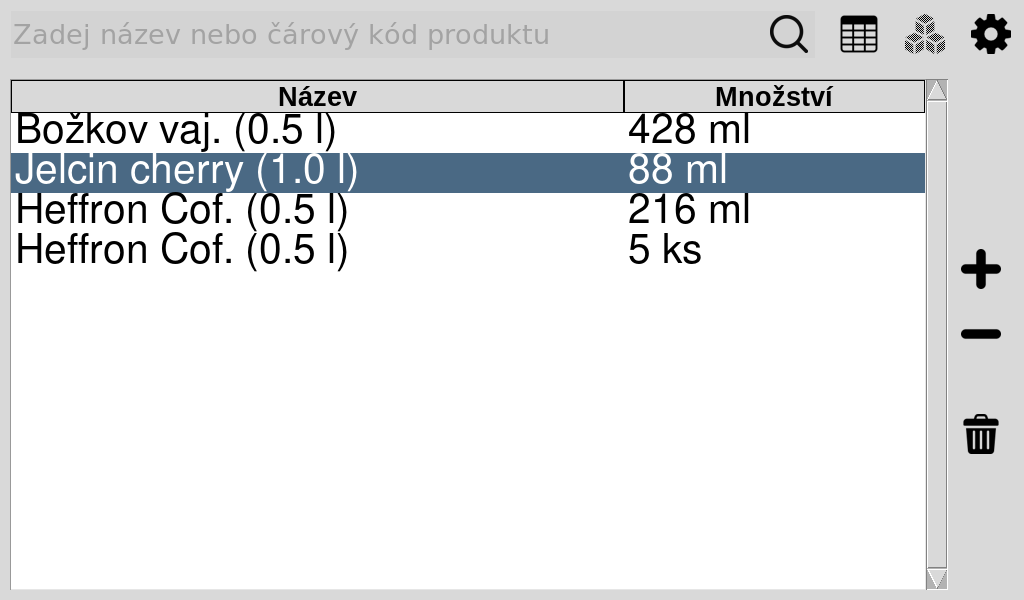
\includegraphics[scale=0.4]{obrazky/GUI Rošířený seznam.png}
    \end{center}
    \caption{Hlavní okno - rozšířený seznam evidovaných produktů}
    \label{Hlavní okno - rozšířený seznam evidovaných produktů}
\end{figure}
//OBRÁZEK - ROZTAŽENÝ SEZNAM

V případě naskenování či vyhledání již evidovaného alkoholu program přejde do stavu "duplicidity".
%Pokud se pokusíme naskenovat nebo ručně vyhledat produkt, který už byl zaevidován, systém automaticky přejde do stavu \textit{duplicity}.


%Nežádoucí stavy:
%\begin{itemize}
%    \item Chyba EAN kódu - Při načtení EAN kódu, který není uložen v databázi nás program upozornění pomocí \textit{proces} labelu, že EAN kod je chybný a ať to zkusíme znovu
%    \item Duplicidní produkt - Pokud se snažíme vyhledat už evidovaný produkt, tak program přejde do stavu duplicidity, tento stav je rozebrán níže. 
%\end{itemize}

\section{Stav - Duplicitní položka}

%Do tohoto stavu jsme se schopni dostat pouze ze stavu vyhledávání a to díky opětovnému vyhledání již evidovaného produktu. V tomto stavu se nám otevře nové okno ve kterém si můžeme vybrat zda zrušíme aktuální výběr(např. kliknutí vedle v seznamu produktů) a vrátíme se do stavu vyhledání nebo produkt budem evidovat i na dále.

Do tohoto stavu se dostaneme pouze prostřednictvím opětovného vyhledání produktu, který již byl jednou zaevidován. Systém následně otevře nové okno, ve kterém má uživatel na výběr: zrušit aktuální výběr (omylem vybral stejný produkt) a vrátit se zpět do stavu vyhledávání, nebo pokračovat do stavu "Vážení".

%\begin{figure}[H]
%    \begin{center}
%        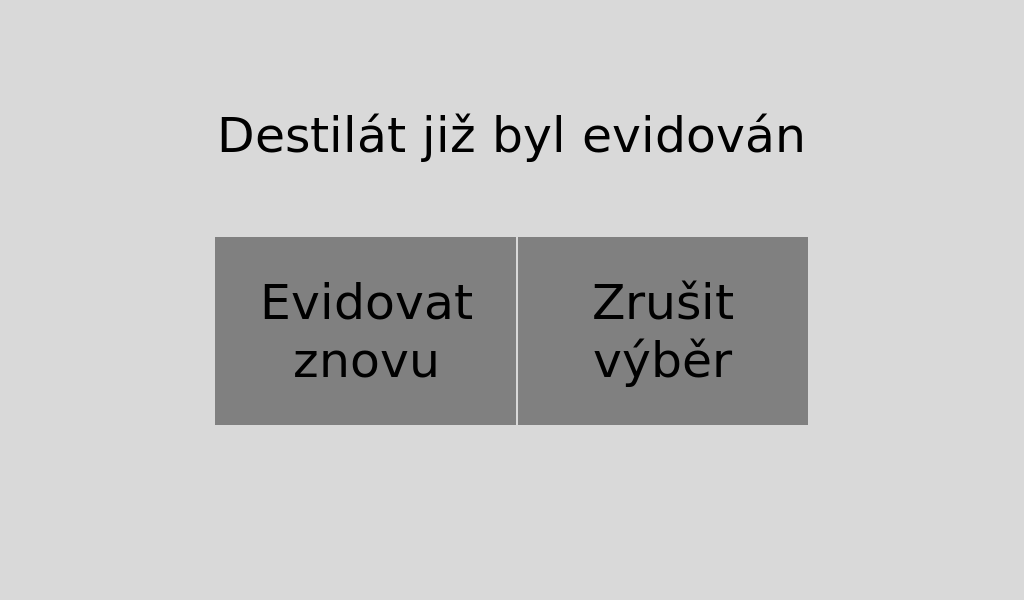
\includegraphics[scale=0.4]{obrazky/GUI Duplicidita.png}
%    \end{center}
%    \caption{Okno informující o duplicitní evidenci produktu}
%    \label{Okno informující o duplicitní evidenci produktu}
%\end{figure}

Opětovná evidence již zaevidovaného produktu má své opodstatnění ve dvou případech:
\begin{itemize}
    \item Pokud máme více rozpitých lahví stejného druhu.
    \item Pokud chceme kromě zbytku z lahve zaevidovat také stav skladu, konkrétně počet neotevřených kusů. K tomu slouží tlačítko pro evidenci kusového zboží s označením btn.stav[xx]
\end{itemize}
%1) Máme více rozpitých lahví
%2) Nechceme evidovat pouze zbytkový objem jedne lahve, ale i stav dané položky ve skladu, tedy počet nenačatých lahví. K tomu slouží tlačítko pro evidenci kusového zboží "btn.stav"[xx]

%Zde muže byt ojeb: Říct že to program hlasí za dvou stavů, když je duplicitní alkohol pouze při zbytkovém objemu ap ak sparatně duplicitní alkohol při kusovém zadávání. Tedy pokud mam alkohol evidovaný pod objemem a chcu ho zadat kusově, tak na tohle nebudu upozorněn protože jsem ho kusově ještě nezadával a to stejný i naopak.

%Chybové hlášení duplicidity:
%Tím, že jsem doposud nechal čtečku běžet v continual modu, tak neustale skenovala a jen při vstrupu od stavu vyhledani jsem čistil vstupní buffer. Ted přepinam mezi countinual a manual režimem, tedy kdžy se dostan do chybové hlašení, tak musím čtečku vypnout protože by četla dal, ale už bych nečistil buffer, takže by se možná hodil novy stav ve kterem bych při zapinal a vypinal čtečku čarovoho kodu, ale to je jen den řadek kodu vlastně no.  

//OBRAZEK - HL. MENU S PRVKY VE ZKRACENEM SEZNAMU
//OBRAZEK - HL. MENU S ROZTAŽENÝM SEZNAMEM
//OBRÁZEK - JAK VYPADÁ RUČNÍ VYHLEDÁNÍ = LISTBOX + KBW
//OBRÁZEK - DUPLICIDITA ZBOŽÍ

\section{Stav - Vážení}
% Obecny popis
Vstupem do tohoto stavu je potvrzena úspěšná identifikace destilátu – buď načtením pomocí EAN kódu, nebo jeho ručním vyhledáním. Zobrazí se detailní informace o daném alkoholickém nápoji:
\begin{itemize}
    \item label Název - Název vyhledaného produktu.
    \item label Hmotnost - Celková hmotnost lahve.
    \item label Max. objem - Maximální objem lahve. Tato informace slouží rozeznat stejný typ destilátu v různých velikostech (0,5 l; 0,7 l; 1 l).
    \item Zbytkový objem - Přepočítaná hmotnost na zbytkový objem v láhvi.
    \item Canvas nyní ukazuje obrázek vybraného produktu. Důvodem je že prodejci, i když né často, mění designe svých lahví a to sebou nese i změnu jejich hmotnosti, v takovém případě je nutné aktualizovat databázi pro daný produkt. U značky a typu lahve \textit{Becherovka originál} (0,5 l) došlo k rozdílu hmotnosti 43 g, díky obměně designu. 
\end{itemize}
\bigskip
Tlačítko pro ukončení inventury se změnilo na "Vrátit zpět" pro případ, že uživatel zvolil špatný produkt.

\begin{figure}[H]
    \begin{center}
        \includegraphics[scale=0.4]{obrazky/GUI Odeberte láhev.png}
    \end{center}
    \caption{Hlavní okno s ukázkou vážení}
    \label{Hlavní okno s ukázkou vážení}
\end{figure}

\subsection{Podmínky vážení}
% Podmínky a omezení - Špatná lahev
Důležitou podmínkou pro správné zvážení je použít správnou láhev. Krom názvu a obrázku produktu je uživatel informován, pokud nastala podmínka:
\begin{itemize}
    \item \textbf{naměřená hmotnost je menší než hmotnost prázdné láhve} - Proto aby se mohl uložit nově naměřený objem do databáze je nutné, aby naměřená hmotnost byla větší nebo rovna než hmotnost prázdné láhve v opačném případě vyjde objem záporný (na displeji se zobrazí jako nulový) a systém čeká než se hmotnost dostane do požadovaného rozsahu.
    \item \textbf{naměřená hmotnost je větší než hmotnost plné láhve} - V moment kdy je naměřená hmotnost vyšší než hmotnost plné láhve se nám do Proces labelu vypíše chybové hlášení: "a.. Maximální hmotnost plné lahve byla překročena." a Label pro zbytkový objem vypíše: "MAX". V tento moment na váze je položená špatná láhev nebo cizí těleso a systém opětovně čeká než se hmotnost dostane do požadovaného rozsahu.
\end{itemize}

\subsection{Stabilizace váhy}
%Stabilizace váhy
Dalším z důležitých faktorů pro určení finálního naměřeného objemu je stabilizovaná váha. Váha sama o sobě signalizuje svou stabilitu tím, že k posílaným datům přes sériovou linku přidá jednotku hmotnosti [X]. V momentě, kdy je váha stabilizovaná a je v požadovaném rozsahu se text objem uloží do databáze a program se přesune do stavu \textit{"remove\_bottle"}. Uživatel je také o úspěšné stabilizaci váhy informován tím, že pozadí labelu zbytkového objemu se obarví do zelena. 

\subsection{Zadání kusového zboží}
\label{sec: Zadání kusového zboží}
%Zadání kusového zboží
Další z funkcí tohoto systému je evidence neotevřených lahví ve skladu, pomocí tlačítka "kusové zboží" nebo také "sklad". Tato funkce nebyla puvodne zamýšlena, ale po otestování systému v praxi se zjistilo, že je nepraktické některé informace vést do systému (naměřený zbytkový objem) a některé na papír - v praxi to znamená, že člověk krom zbytkového alkoholu uvádí i aktuální stav ve skladu. Proto přibilo toto tlačítko. Po jeho stisknutí se nám oblast s informacemi o zbytkovém objemu (label č1, label č2) překryje numerickou klávesnicí pro zadání počtu kusového zboží. %(možné použít pouze ve stavu vyhledání sortimentu, ale nesmí být aktivovaná rozšířená tabulka)

\begin{figure}[H]
    \begin{center}
        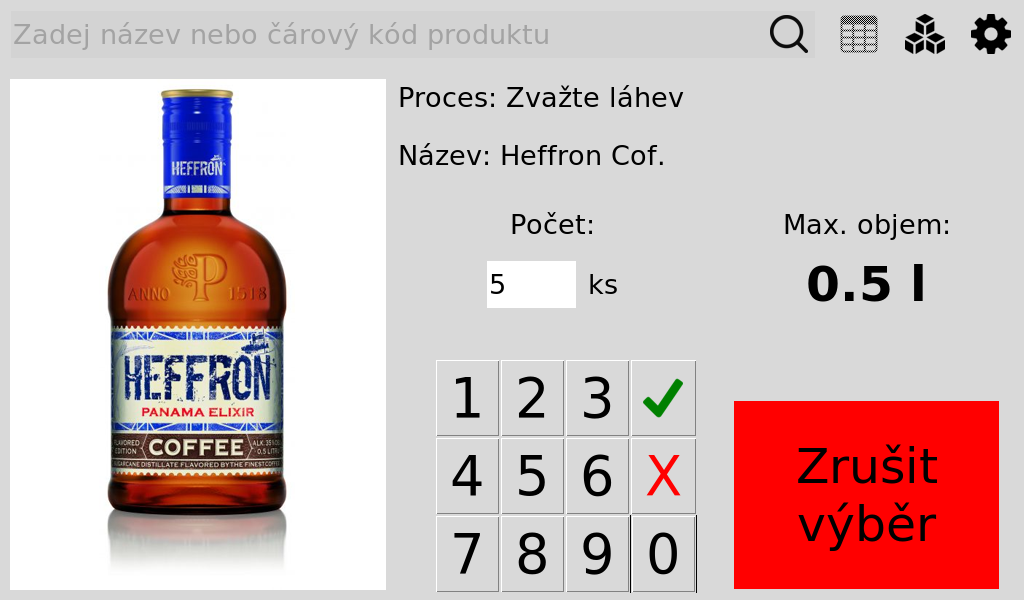
\includegraphics[scale=0.4]{obrazky/GUI Numericka klavesnice.png}
    \end{center}
    \caption{Hlavní okno - zadání kusového zboží ze skladu}
    \label{Hlavní okno - evidence kusového zboží ze skladu}
\end{figure}

%Tato funkce nebyla původně zamýšlená, ale z praktického hlediska jsem ji dodal, protože po otestování systému v praxi vyzněla myš

%\subsection{Použití nalévačů}
% Nevyuití nalévačů
%Další úprava která mě dovedla po otestování systému bylo odstranění původně zamýšlené databáze nalévačů.
%Po otestování systému v praxi se ukázalo, že je nepraktické vést databázi s hmotnostmi různých nalévačů a snažit se převést schopnost v jejich výběru pomocí GUI. Implementace nalévačů do programu, proběhlo dvoumi způsobi:
%1) V hlavním okně jsem vytvořil zaškrtávací políčko, které informovalo zda nalévač je na lahvi či nikoli a každý alkohol měl přidělený ve své databázi svůj nalávač, pokud to bylo nutné změnit přiřazení nalévače dělalo se to přes databázi. bohužel se ukázalo, že s každou inventurou se nalévače na lahvích mění nebo tam nejsou vůbec, proto bylo nepraktické nastavit fixně jeden typ nalevače na jednu láhev. Jednou z možných řešení bylo mít na každou lahev stejný tyto nalévače, ale to pro personal bylo nepraktické a tak je začali sundávat.
%2) Udělal jsem inovaci v tom, že před každou evidenci lahve tedy před jeho navážením zaměstnanec musel vybrat typ nalévače pro danou lahev ze seznamu, který mu vyjel pod Entry oknem, kde bylo přidáno přepínací tlačítko mezi seznamem produktů a nalévačů. Tato metoda se nakonec ukázala jakou zdlouhavá a proto byla odstraněna. Mnohem rychlejší bylo nalévač sthrnout z hrdla lahve a navážit bez něj než ho hledat v seznamu kvuli kompenzaci jeho hmotnosti. Tudíž na základě tohoto všecho jsem odstranil i databázi veškerých nalévačů.

%Po otestování systému v praxi se ukázalo, že je nepraktické vést databázi s hmotnostmi různých nalévačů. V provopočátku některé detiláty měli přiřazený svůj nalévač fixně a uživatel mohl použít zašktrtávací tlačíko pro važení s nalévačem či bez. Bohužel s každou inventurou se nalávače na láhvích pravidelně měnily, proto jsem přidal možnost v uživatli si pro daný alkohol za chodu inventury vybrat ze seznamu konrétní nalévač. Toto řešení se moc neosvědčilo a zaměstnanci raději zvolili vážení bez nalévače a raději ho strhly, protože to pro ně bylo rychlejší než jej hledat v seznamu nebo kontrolovat zda použitý nalévač na láhvi odpovídá nalévači přiřazeného k danému destilátu. Na základě této zkušenosti jsem odebral tuto databázi a možnost vážit s nalévačem. Využití vážení s nalévačem by bylo za předpokladu, že by podnik měl na všechny láhve stejný typ nalévače a nemusel by se zdržovat kontrolou správného typu, pouze voulbou možnosti vážení s nalévačem či bez. Tato řešení se ale neosvěčilo, protože pro zamestnavatele bylo přivětivější nákup nalévačů, které byly zrovna cenově dostupné než řešit nepatrný rozdíl hmotnosti zpusobené špatným nalévačem.


%V tomto stavu nám zbývá navážit zbytkový objem a nebo zadat počet kusů. V tomto satvu jak vidite nam se přejmenovalo tlačítko z ukončení inventury na zpět, tedy mlžeme zrušit náš výběr destilátu v případě chybného zadání ručně např. nebo jsme prostě naskenovali něco co jsme evidovat nechteli.

%//obrazek - vážení destilátu
%//obrázek - zadávání kůsů


\section{Stav - Nastavení aplikace}
\label{sec:Nastavení aplikace}
Do nastavení se dá dostat v libovolném stavu programu pomocí ozubeného tlačítka. V teto fázi jeste neni dodelane veskre funkce nastavení pouze její vizuál.

Nastavení by mělo poté umožňovat:
Ve finální verzi by nastavení mělo umožňovat:
-Doplneni databaze
-Zpetna kontrola inventury
-nastaveni hesla pro administratorsky pristup
-Nastavení jednotek hmotnosti a objemu
-nastavení jazyku
-nastavení nočního režimu

%\begin{figure}[H]
%    \begin{center}
%        \includegraphics[scale=0.4]{obrazky/GUI Nastavení.png}
%    \end{center}
%    \caption{Okno s nastavením aplikace}
%    \label{Okno s nastavením aplikace}
%\end{figure}


\section{Stav - Konec inventury}

%Pro ukončení inventury je nutné, aby uživatel zadal jméno zaměstnance ze seznamu (dropboxu), kde jsou evidovaní všichni zaměstanci, co můžou vykonávat inventůru, tedy tímto se zaměstnanec podepíše pod svou vlastní inventutu, kterou vykonal, jedná se o bezpečnostní prvek, aby bylo možné v případě nejasností v inventuře dohledat, kdo danou inventuru vykonal. Pokud jmeno nezadáme aplikace nás vyzve k jeho zadání a nepustí nás dál, v opačném případě nás přesměruje na obrazovku, kde se nás zeptá zda jsme si jistí tím, že chceme inventuru ukončit (bezpečností prvkek, kdyby jjsme omilem klikli na ukočení inventury). Po uspěšném ukončení inventury se nám obrazovka přene zpátky na výchozí obrazovku[xx]

%Pro ukončení inventury je nutné, aby uživatel zadal jméno zaměstnance ze seznamu (dropboxu), kde jsou evidovaní všichni zaměstanci, co můžou vykonávat inventůru, tedy tímto se zaměstnanec podepíše pod svou vlastní inventutu, kterou vykonal, jedná se o bezpečnostní prvek, aby bylo možné v případě nejasností v inventuře dohledat, kdo danou inventuru vykonal. Pokud jmeno nezadáme aplikace nás vyzve k jeho zadání a nepustí nás dál. Aktuálně spuštěnou inventuru lze i vymazat např. z důvodu milného spuštění, následně čeká ověřovací okno zda jsem si jistí tímto rozhodnutím. Ať při ukončrní inventury nebo jejího vymazání nás applikace přesměruje zpátky na úvodní obrazovku.

Před samotným ukončením inventury musí uživatel vybrat jméno zaměstnance ze seznamu (rozbalovacího pole), který obsahuje všechny pracovníky oprávněné k provádění inventur. Tento krok slouží jako forma elektronického podpisu – určuje, kdo konkrétní inventuru provedl, což je důležité pro zpětnou dohledatelnost v případě jakýchkoliv nesrovnalostí. Pokud jméno není zadáno, aplikace na tuto skutečnost upozorní a nepovolí pokračovat dále.

V případě, že byla inventura spuštěna omylem, je možné ji zcela vymazat. Před provedením tohoto kroku se zobrazí potvrzovací dialog, který slouží k ověření, zda je uživatel smazáním skutečně jistý.

Po ukončení nebo smazání inventury je uživatel automaticky přesměrován zpět na úvodní okno aplikace (Stav 1).


\begin{figure}[H]
    \begin{center}
        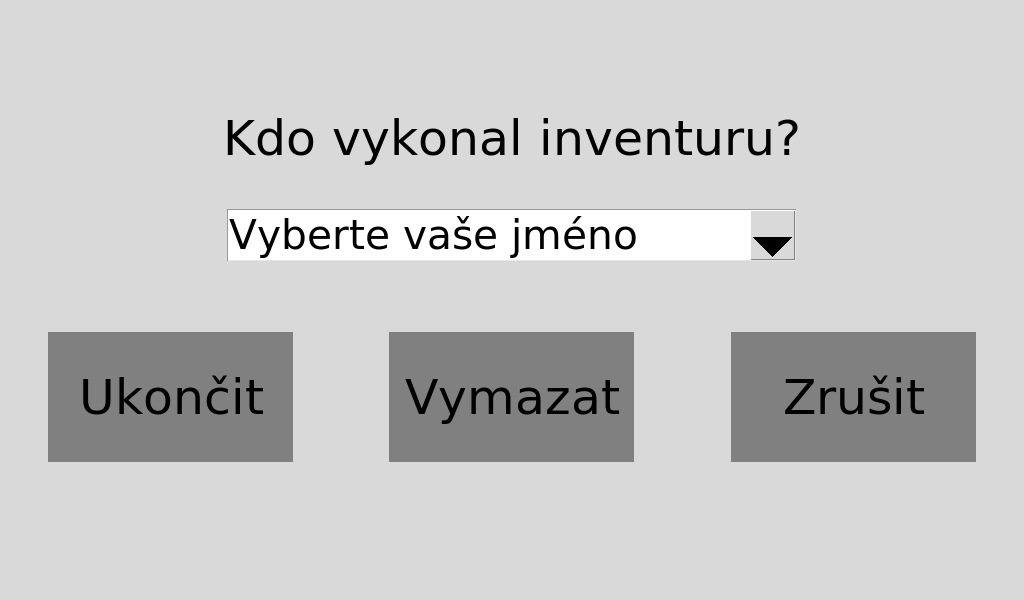
\includegraphics[scale=0.4]{obrazky/GUI Konec inventury.png}
    \end{center}
    \caption{Ukončovací okno aplikace}
    \label{Ukončovací okno aplikace}
\end{figure}

%\begin{figure}[H]
%    \begin{center}
%        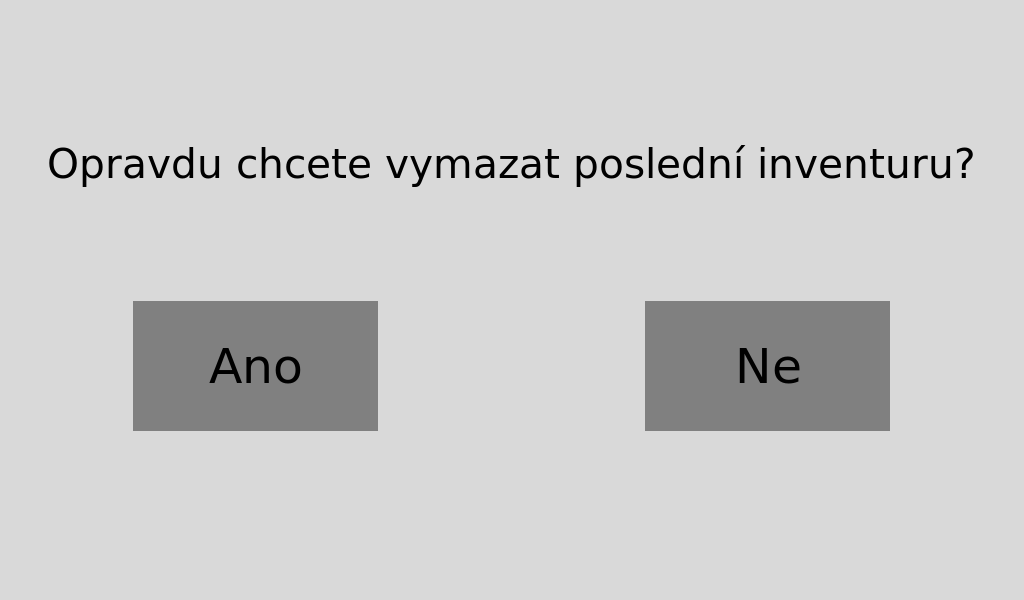
\includegraphics[scale=0.4]{obrazky/GUI Vymazání inventury.png}
%    \end{center}
%    \caption{Potvrzovací okno pro vymazání aktuálně spuštěné inventury}
%    \label{Potvrzovací okno pro vymazání aktuálně spuštěné inventury}
%\end{figure}

\section{Zdrojový soubor grafického prostředí - gui.py}
%V této sekci se zaměříme na programové řešení modulu \texttt{gui.py}. grafické prostředí aplikace je rozděleno do x tříd z důvodu přehlednosti a orientaci v kódu. jedna co ma nastarost vykreslování veškerých oken a další kod, co byl více komplexnejsi, tak jsem zaobalil do vlastní třídy a to třídu pro klavesnici a listbox obsahující seznam destilátů, protože samy o sobě obsahuji dosti kodu, ktery by delal hlavní třídu nepřehlednou. Tyto třídy jsou navzájem provázané pomocí klíčového slova Parent, neboli třida Keyboard a Listbox dědí z hlavní třídy pomocí toho klíčového slova. Parent předává není přímo objekt, je pouze proměná s adresou v paměti na naši hlavní třídu, tedy mužeme skrz toto slovo přistupovat do existujícího objektu.. Nástroj/třída/modul tkinter může vytvořit pouze jedno hlavní okno pomocí klíčového slova tk, tk je třída hlavního okna v programu může být vytvořena jen jednou mé tříde dědím právě ne z třídy, ale modulu..hovno přímo z třídy tk, tudíž mi klíčové slovo self. umožnuje přistupovat k proměným dané třídy tedy i k proměným děděné třídy. tedy pro vytvořeí hlavního okna..ho musím prvně setupunout a pak metodou .mainloop() spusttí hlavní smyčku programu, abych ale mohl komunikovat s dalšími i s jinými třídami a stavovým automatem jako čtečkou a váhou, tak musím z této smyčky i vyskočit, pro tyto účely je metoda after(), proto v mainu ve funkci stavového automatu, opakovaně volám funkci sebe samou

%nevyhodou Pythonu je, že všechny interní proměnné třídy se musí inicializovat uvnitř konstruktoru což v nšem případě, kde máme hromadu ovladacích prvků činí samotnou třídu nepřehlednou a v případě deklarovani promenné v blízkosti metody by se z ní stala statická proměnná. 

%//Ukazka kodu
%Hlavní třída GUI, dědí z třídy Tk, která vytváří hlavní okno programu. V hlavní okno je rozděleno do dvou rámců/framů pro jednoduší vkládání ovládacích prvků. Jedna z metod pro vkládání je grid(), která umožnuje prvky skládat do sloupců a řádku, které mezi sebou interagují a udržují symetrický vzhled. Tudíž třeba když jeden sloupec prvků roztáhnu, ostatní se smrští a prvky se nebudou překrývat přes sebe - dynamické nastavení. Třídy jsou velice rozsáhlé, proto jen vypíchnu to nejduležitějšší.

Táto sekce je zaměřená na programové řešení modulu \texttt{gui.py}. Grafické prostředí aplikace je rozděleno do x tříd z důvodu přehlednosti a orientaci v kódu. Hlavní okno je reprezentováno třídou \texttt{MainWindow}, dědící ze třídy \texttt{Tk}, které spouští hlavní smyčku programu. MainWindow vytváří instanci ostatních tříd, které obsahují kód ostatních oken nebo jinou složitější část kódu. Pro vytvoření nového okna se používá třída \texttt{Toplevel}, které je prostřednictví parametru master přiřazen přídružné okno ke kterému se vztahuje. V případě vyvíjené aplikace jsou všechna Toplevel okna odkázána na hlavní okno. V praxi je spouštěno pouze jedno hlavní okno a libovolný počet Toplevel oken. Jak už bylo jednou zmíněno pro vyskočení z hlavní smyčky za účelem periodických operací (chod stavového automatu, obsluha portů, atd) se využívá metoda after[].

Hlavní okno se skládá ze dvou grafických rámců (tk.Frame) horizontálně rozdělených, kde jeden obsahuje ovládací prvky Entry, a tlačítka pro nastavení, numerickou klávesnici a rozšíření seznamu evidovaných položek. Druhý rámec představuje zbytek okna. Pro vkládání ovládacích prvků do prostředí je využita metoda grid, která umožňuje rozdělit daný rámec na mřížku, kde jednotlivé řádky a sloupce mezi sebou interagují a udržují symetrický vzhled prostředí.



\begin{lstlisting}[language=Python, caption=Funkce stavového automatu, frame=single, breaklines=false]
class MainWindow(tk.Tk):
    def __init__(self):
        super().__init__()
                        ...                       
        self.StartWindow: tk.Toplevel = None
        self.EndWindow: tk.Toplevel = None
        self.SameDest: tk.Toplevel = None
        self.DeleteWindow: tk.Toplevel = None
        self.Settings: tk.Toplevel = None
        self.Keyboard: tk.Toplevel = None
        self.ListBox: tk.Toplevel = None
                        ...
\end{lstlisting}

Ostatní třídy jsou definované stejným způsobem. Ukázka na třídě Keyboard. Třída keyboard dědí ze třídy Toplevel, což je vytváření sekundárních oken GUI, tato třída je provázána s třídou GUI pomocí parametru root. Toplevel, tedy Toplevely mohou odkazovat přímo na hlavní okno nebo jiný Toplevel, předání parametru je pomocí konstruktoru super().\_\_init\_\_(root)

%\begin{lstlisting}[language=Python, caption=Funkce stavového automatu:, frame=single, breaklines=false, postbreak=\mbox{\textcolor{gray}{$\hookrightarrow$}\space}]
%
%class Keyboard(tk.Toplevel):
%    def __init__(self, root:GUI):
%        super().__init__(root)
%        self.root = root
%        self.geometry("1024x600")
%        asd
%        asd
%        as
%        da
%        sd
%        asd
%        as
%        da
%        sda
%        sd
%        asd
%        asd
%        asd
%        
%\end{lstlisting}


\section{Zdrojový soubor databáze - database.py}

Modul \textbf{database.py} zajišťuje trvalé ukládání a vyhledávání údajů o lahvích a inventurních měřeních do relačních databázích \textbf{database.db} a \textbf{inventory.db} uložených lokálně na SD kartě Raspberry Pi. Databáze se dále skládají z tabulek (table) stejně jako Excel se skládá z více listů. Soubory s příponou \textbf{.db} jsou čitelné pro databázový engine SQLite, který umí databázový jazyk SQL. Aby byla práce s daty v Pythonu přehlednější, je využit nástroj (modul) SQLAlchemy:
\begin{itemize}
    \item SQLAlchemy vytváří nad SQLite enginem objektovou vrstvu (ORM).
    \item Každou tabulku mapuje na Python třídu – aplikace tak pracuje s atributy objektů místo ručního skládání příkazů SQL.
    \item Umožňuje jednoduchý přechod na jiný databázový systém (např. \textit{PostgreSQL})
\end{itemize}

\begin{lstlisting}[language=Python,breaklines=false, frame=single, caption=Ukázka třídy database.db a inventory.db]
Chyba latexu
\end{lstlisting}

\subsection{Práce se souborem database.db}
Soubor database.db obsahuje 2 tabulky:
\begin{itemize}
    \item destilate - seznam destilátů a jejich parametry [č.x]
    \item employee\_name - seznam jmen zaměstnanců možných vykonávat inventuru
\end{itemize}
Pro vyhledání konkrétního destilátu se používají 2 funkce:
\begin{itemize}
    \item get\_info\_by\_ean - vyhledá produkt na základě jeho EAN kódu
    \item get\_info\_by\_name - vyhledá produkt na základě jeho názvu
\end{itemize}
\begin{lstlisting}[language=Python,breaklines=false, frame=single]
def get_info_by_ean(ean:str) -> Destilate
\end{lstlisting}
\begin{lstlisting}[language=Python,breaklines=false, frame=single]
def get_info_by_name(name:str) -> Destilate
\end{lstlisting}
V obou případech je návratová hodnota \texttt{Destilate} objekt obsahující veškeré informace vyhledaného produktu.
Pro manuální vyhledávání slouží funkce \texttt{get\_rows\_by\_name}, která prohledá tabulku destilátů na základě vloženého substringu a vrátí list polí 2x1 obsahující název destilátu a jeho maximální objem.
\begin{lstlisting}[language=Python,breaklines=false, frame=single]
def get_rows_by_name(substr:str)->list[tuple[str,float]]
\end{lstlisting}

\subsection{Práce se souborem inventory.db}
Databáze inventory.db obsahuje tabulky, které dále obsahují veškeré naměřené data v rámci jedné inventury.

Metoda \texttt{create\_new\_table} je volána po spuštění inventury a úspěšném průchodu stavem \texttt{check\_port} v mainu, kdy vytvoří novou tabulku s názvem inventory a přiřadí jí datum a čas vytvoření pro zpětnou kontrolu. V případě neuspěšného vytvoření tabulky je vyvolána vyjímka \texttt{Exception}.
\begin{lstlisting}[language=Python,breaklines=false, frame=single]
def create_new_inventory_table() -> None
\end{lstlisting}
\bigskip
Metoda rename\_last\_table je volána při ukončení inventury, kdy za konec jména tabulky se přidá jméno pracovníka pro zpětnou kontrolu.
\begin{lstlisting}[language=Python,breaklines=false, frame=single]
def rename_last_table(name:str) -> None
\end{lstlisting}
\bigskip
Poslední funkcí je delete\_last\_table, která vymaže poslední tabulku v inventory.db, např. z důvodu mylného spuštění inventury.
%vytvořenou aktualně běžící inventuru.
\begin{lstlisting}[language=Python,breaklines=false, frame=single]
def delete_last_table() -> None
\end{lstlisting}

%
%\subsection{hledání dat}
%\subsection{výpis dat}
%\subsection{sdsds}




\section{Zdrojový soubor čtečky čárového kódu - barcode\_sensor.py}
Kamerová čtečka GM65 komunikuje prostřednictvím USBVcom. Čtečka je přepínána mezi čtecími režimi continual a manual viz kapitola č.XXX. 

Kod pro ovládání čtečky je zaobaleno do třídy \texttt{BarcodeSensor} obsažené v modulu \texttt{barcode\_sensor.py}. Třídá dědí ze třídy \texttt{Serial}, která zastřešuje veškerou seriovou komunikaci. Konstruktor třídy BarcodeSensor přebírá parametry pro adresu portu, rychlost seriové komunikace (baudrate) a timeout, který slouží k přerušení zápisu/čtení na daném portu po určitém čase. Tyto veškerý data se následně předají konstruktoru třídy Serial. 

\begin{lstlisting}[language=python,breaklines=true, frame=single]
import serial
class BarcodeSensor(serial.Serial):
    def __init__(self, port=None, baudrate=9600, timeout=1):
        super().__init__(port=port, baudrate=baudrate, timeout=timeout)
\end{lstlisting}
\bigskip
Třída obsahuje metodu \texttt{open\_port}, která otevírá nastavený port pro komunikaci. 
V případě úspěšné otevření vrátí \texttt{True}. 
%Návratovou hodnotou je \texttt{bool} na základě toho, zda se otevření povedlo nebo ne.

\begin{lstlisting}[language=Python,breaklines=false, frame=single]
def open_port(self) -> bool:
\end{lstlisting}

\bigskip
Metoda turn\_on\_sensor přepne čtečku do aktivního stavu, kde se rozsvítí LED dioda, povolí bzučák pro případ naskenování čárového kódu a čtečka přejde do contianul režimu. Opakem této metody je metoda turn\_off\_sensor, kdy čtečka se přepně do manuálního režimu. Předpis datového packetu odesilaného do čtečky se skládá z:

\begin{itemize}
    \item hlavička (head) - Značí odesílatele dat (0xEA 0x00: řídicí jednotka → čtečka)
    \item Zone byte (types) – Typ operace (zápis do čtečky, výpis nastavení, ...)
    \item lens – délka bloku \textit{data} v bajtech
    \item adress – oblast nastavení (typ čtení, rychlost čtení, typ kódu)
    \item data – konkrétní nastavení dané oblasti (zapnutí LED diody, čtecí režim, ...)
    \item CRC – kontrolní součet (XOR) detekující chybnou zprávu. 
\end{itemize}

\begin{table}[H]
    \centering
    \begin{tabular}{|c|c|c|c|c|c|}
         \hline
         Head & Types & Lens & Adress & Data & CRC\\ \hline
         0x7E 0x00 & 0x08 & 0x01 & 0x00 0x00 & 0xEA & 0x?? 0x??\\
         \hline
    \end{tabular}
    \caption{Předpis datového packetu pro aktivaci čtečky}
    \label{tab:my_label}
\end{table}

\begin{table}[H]
    \centering
    \begin{tabular}{|c|c|c|}
         \hline
         Pořadí bitu & Hodnota bitu & Funkce \\ \hline
         7. & 1 & Probliknutí při přečtení kódu \\ \hline
         6. & 1 & Zapnutí bzučáku \\ \hline
         5-4. & 10 & Nastaví se stejně jako 2-3. bit \\ \hline
         3-2. & 10 & Zapnutí LED \\ \hline
         1-0. & 10 & Continual mode (Čtecí režim)\\ \hline
    \end{tabular}
    \caption{Výpis funkcí jednotlivých bitů bloku "Data". 0xEA (HEX) = 11101010 (binary)}
    \label{tab:my_label}
\end{table}

%\begin{lstlisting}[language=Python, caption=Metoda turnooonoosensor, frame=single, breaklines=false, postbreak=\mbox{\textcolor{gray}{$\hookrightarrow$}\space}]
%
%def turn_on_sensor(self) -> bool:
%
%    data_on = bytes([0x08, 0x01, 0x00, 0x00, 0xEA])
%    crc_on = self.crc16_ccitt(data_on)
%    crc_on_high = (crc_on >> 8) & 0xFF
%    crc_on_low = crc_on & 0xFF
%           
%    scan_command:bytes = bytes([0x7E, 0x00]) + data_on + bytes([crc_on_high, crc_on_low])
%    self.write(scan_command)
%    ack:bytes = self.read(7)
%
%    if ack == bytes([0x02, 0x00, 0x00, 0x01, 0x00, 0x33, 0x31]):
%        return True
%    else:
%        return False
%\end{lstlisting}
\bigskip
Metoda \texttt{crc16\_ccitt} vykonává kontrolní 16 bitový součet z bloků \textit{Types} až \textit{Data}. Výstupem je 16 bitové číslo, které je následně rozděleno na 2 separátní bajty.[zdroj1]
%https://srecord.sourceforge.net/crc16-ccitt.html

%\begin{lstlisting}[language=Python,breaklines=false, frame=single,postbreak=\mbox{\tiny$\hookrightarrow$}]
%
%def crc16_ccitt(self, data: bytes, poly=0x1021, crc=0x0000) -> int:
%    for byte in data:
%        crc ^= (byte << 8)
%        for _ in range(8):
%            if (crc & 0x8000):
%                crc = ((crc << 1) ^ poly) & 0xFFFF
%            else:
%                crc = (crc << 1) & 0xFFFF
%\end{lstlisting}
\bigskip
Jako poslední metoda je \texttt{read\_sensor\_data} která posílá nazpět naskenovaná data uložená ve vstupním bufferu mikropočítače.
%\begin{lstlisting}[language=Python,breaklines=false, frame=single,postbreak=\mbox{\tiny$\hookrightarrow$}]
%
%def read_sensor_data(self) -> str:
%    if self.in_waiting == 0:
%        return ''
%    return self.read(15).decode()
%\end{lstlisting}

\section{Zdrojový soubor váhy - scale.py}
\label{sec: scale.py}
Digitální váha G\&G E3000 komunikuje po linkách TX/RX standardu RS‑232 ve formátu 8 N 1 a baudrate 9600 Bd. Aby bylo možné váhu připojit k jednodeskovému počítači Raspberry Pi 4, je rozhraní převáděno adaptérem AXAGO ADS‑50 na virtuální COM port USB CDC (obr. 6‑3). Pro tuto váhu byla vytvořena třída Scale zastřešující veškero serivou komunikaci váhy s mikropočítačem. Konstruktor třídy přebírá parametry pro nastavení portu, baudrate a timeout který nastavuje, čtení na seriovém portu po dobu 1 s. Pokud do tohoto intervalu nejsou zaznamenány žádné příchozí data, čtení se ukončí. Třída dále dědí ze třídy serial, které předává všechny zmíněné parametry.

\begin{lstlisting}[language=Python,breaklines=false, frame=single]
class Scale(serial.Serial):
    def __init__(self) -> None:
        super().__init__(baudrate = 9600, timeout=1)
\end{lstlisting}

\subsection{Ověření komunikace s váhou}
Aby bylo možno s váhou komunikovat je nutné otevřít port na kterém je připojena a to pomocí metody \texttt{open\_port}, která je volána z druhého stavu v mainu. V případě chyby se vyvolá výjimka xxxa a metoda vrátí \texttt{False}.

\begin{lstlisting}[language=Python,breaklines=false, frame=single]
def open_port(self) -> bool:
\end{lstlisting}

Po úspěšném otevření portu se zkontroluje zda váha komunikuje (není vypnutá) pomocí metody \texttt{check\_conection} tím že pošle příkaz \textbf{0xBH 0x70} a váha odpoví kolik navážila, předpis ACK zprávy je ve tvaru [sss].

\begin{lstlisting}[language=Python,breaklines=false, frame=single]
def check_conection(self) -> bool:
\end{lstlisting}

\subsection{Komunikace s váhou po sériové lince}

Ke komunikaci slouží metoda  \texttt{print\_scale}, která odesílá stejnou zprávu jako metoda \texttt{check\_conection}, pokud ale váha neodpoví do stanoveného času pomocí timeoutu zkontroluje se zda je port otevřený, pokud není metoda vrátí \textit{Err1} a pokud je metoda vrátí \textit{Err0}.

\begin{lstlisting}[language=Python,breaklines=false, frame=single]
def print_scale(self) -> str:
\end{lstlisting}
Problém je že váha neposílá žádný kontrolní znak a ani neobsahuje paritu, proto abychom se ujistili, že příchozí data nejsou poškozena budem kontrolovat zda poslední 3 přijaté zprávy jsou shodné dle stavového diagramu \ref{ošetření parity}. Kontrolovat budem pouze zprávy které došli s jednotkou hmotnosti, čímž váha říká, že je stabilizovaná. Důvodem je, že pokud zatížíme váhu, tak její naměřená hmotnost se velice rychle mění, proto bysme nedokázali přijmout v této fázi 2 stejné hodnoty hmotnosti posobě v rámci kodu jsou zpracovávána pouze stabilizovaná data.

%% NÍŽE VYMAZAT VŠE

%%stavák ošetření stavového automatu
%\begin{figure}[H]
%    \begin{center}
%        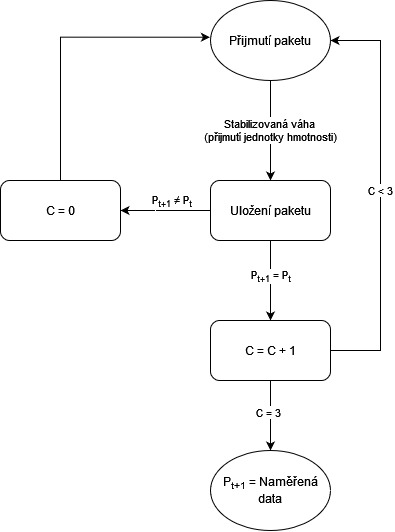
\includegraphics[scale=0.6]{obrazky/stavovy_automat_parita.jpg}
%    \end{center}
%    \caption{Kontrola příchozích zpráv z váhy}
%    \label{ošetření parity}
%\end{figure}
%
%
%navíc do databáze se ukládají až stabilizované hodnoty, proto
%
%
%
%
%Tok dat směřuje obousměrně – váha odesílá měřené hodnoty, řídicí jednotka je v intervalech \~200 ms vyžaduje řídicím párem znaků ESC 'p'. Třída Scale zastřešuje veškero serivou komunikaci váhy s Raspberry Pi. Třída dědí ze třídy Serial, kde v jejím konstruktoru nastavujeme baudrate 9600 a timeout=5s. 
%
%Metoda open\_port() je volána z druhého stavu v mainu, která otevírá serivový port pro komunikaci v případě selhání vyhodí vyjímku vrátí hodnotu False.
%
%Dále je metoda check\_conection(), která se volá po uspěšnem otevření portu a kontroluje zda váha komunikuje, tím že pošle příkaz na ve tvaru esc+p a váha odpoví kolik navážila, pokud jsou data přijata (je jedno co pošle), tak váha komunikuje.
%
%Nejduležitší metodou je print\_scale(), která odesílá požadavek na "tisk" dat. Tím, že váha neposílá paritní bit, děláme SW kontrolu, zda 3 poslední zprávy jsou shoné pomocí stavového diagramu obrč.x
%
%\begin{lstlisting}[language=Python, caption=Funkce stavového automatu:, frame=single]
%def print_scalee(self) -> str:
%\end{lstlisting}

\section{Spouštěcí script}
\section{Splash obrazovka}
\section{Praktická úkázka}
Hodit sem fotku celého systému

Pak sem hodit fotku malého odměrného válce s vysokou přesností a porovnat to s fotkou kde jsem navážil stejný objem - at jde vydet hlavne lahev na váze + displej váhy, pak celý displej, jestli ukazuje stejnou hmotnost + nove vypočítaný objem.

Mozna udelat aj nejaký výpočet
%7. Na vhodném příkladu odzkoušejte, ověřte a demonstrujte funkčnost celého systému.

%započítat čas i zápisu do papíru (než se najde položky muže to trvat)

%otestovat zatížení programu (podivat se do spravce uloh)
%zkusit vymyslet nějaký testy, kde se něco časuje

%Sundání nalévače většinou zabralo 1 - 2 s a našroubování víčka
\chapter{Otestování nově navrženého systému}
%\chapter{Otestování měřícího systému}

%Tato kapitola se bude zabívat testo
Tato kapitola se bude zabývat testováním navrženého systému jako celek. Testování bylo rozděleno do dvou kategorií, v jedné je test rychlosti měření, tato měření jsou podložena videem obsaženým v elektronické příloze, dokazující funkčnost systému a ukázku provedení inventury. Druhé testování ověřuje stanovenou přesnost $\pm$10 ml měřicího systému z kapitoly č. \ref{sec:chyby měření}.
%Druhé testování ověřuje stanovenou přesnost měřicího systému a to $\pm$10 (viz kap. č. \ref{sec:chyby měření}).


%Uvest sem tip na ověření systému

%%%%%%%%%%%%%%%%%%%%%%%%%%%%%%%%%%%%%%%%%%%%%%%%%%%%%%%%%%%%%%%%%%%%%%
%1. 10 lahví - obyc + alc válec
%2. Měření kazdé lahve zvlášť v příloze, zde jen výsledek
%3 video které toto dokazuje (10 naměřených lahví)
\section{Doba inventury po implementaci nově navrženého systému}

%Měřicí systém byl testován s odměrnými válci na lahvi různých zbytkových objemů
Měření časové úspory navrženého měřicího systému vůči odměrným válcům proběhlo ve dvou fázích.

V první fázi byla měřena jedna láhev různých zbytkových objemů - to se projeví pouze u odměrného válce, kde je nutné přelévat destilát. Výsledky jsou uvedeny v tabulce č. \ref{tab:cas_mereni}, kde je vidět, že měřicí systém opravu zrychlil proces měření zbytkového objemu o x \% u odměrného válce s nutností přelévání a x \% u odměrného válce na alkohol.

%U měřicího systému byl měřen čas (zhruba 1 s) včetně sundání nalévače (viz kap. č. x).
%U měřicího systému byl do času měření započteno i sundání nalévače (viz kap. č. x), doba sundání je 

\begin{table}[H]
    \centering
    \newcolumntype{C}[1]{>{\centering\arraybackslash}m{#1}}
    %\renewcommand{\arraystretch}{1.2}   % zvětší řádkování v tabulce
    \begin{tabular}{|c|C{2,7 cm}|C{2,7 cm}|C{2,7 cm}|}
        \hline
        & \multicolumn{3}{c|}{Čas [s]} \\ \hline
        \begin{tabular}[c]{@{}c@{}} Zbytkový objem \\ v lahvi [l] \end{tabular} & \begin{tabular}[c]{@{}c@{}} Odměrný \\ válec \end{tabular} & \begin{tabular}[c]{@{}c@{}} Odměrný válec \\ na alkohol \end{tabular} & \begin{tabular}[c]{@{}c@{}} Navržené \\ zařízení \end{tabular} \\ \hline \hline
        0,1   &            & \textbf{---}          & \textbf{---}           \\ \hline
        0,5 &            & \textbf{---}         & \textbf{---}         \\ \hline
        1 &            &          &          \\ \hline
    \end{tabular}
    \caption{Časová náročnost měření zbytkového objemu v lahvi pomocí odměrných válců a pomocí navrženého měřicího systému}
    %\caption{Měření doby měření zbytkového objemu v lahvi pomocí odměrných válců a měřicího systému}
    \label{tab:cas_mereni}
\end{table}

%Druhé měření testovalo použití systému při inventuře
%Ve druhé fázi byl měřen čas provedení inventury, kdy na baru bylo 12 lahví.
Ve druhé fázi byl systém otestován v provozu při standardní/běžné inventuře, kdy na baru bylo 12 lahví. V praxi se prvně změřily všechny lahve odměrným válcem na alkohol, pro které existovala stupnice na válci (4 lahve), poté zbylé lahve obyčejným odměrným válcem (8 lahví). Lahví ve skutečnosti je na baru více, ale pokud pro ně není žádná tržba, tak se jejich zbytkový objem neměří, pouze se přepíše z minulé inventury. Výsledky měření ukázaly, že využití měřicího systému zkrátilo vykonání inventury o x \% (viz tab. č. \ref{tab:delka_inventury}). Video obsahující toto měření pomocí navrženého měřicího systému je obsaženo v elektronické příloze pod názvem: "ukázka funkčnosti měřicího systému.mp4".
%Video obsahující naměření těchto 12 lahví pomocí navrženého měřicího systému je obsaženo v elektronické příloze.

%V elektronické příloze je dodáno video 


%Druhé měření testovalo použití systému při inventuře, kdy na baru bylo otevřeno 12 lahví. V praxi se změří všechny lahve odměrným válcem na alkohol pro které existuje stupnice na válci (4 lahve), až potom obyčejným odměrným válcem (8 lahví). Lahví ve skutečnosti je na baru více, ale pokud pro ně není žádná tržba, tak se jejich zbytkový objem neměří, pouze se přepíše ten z minulé inventury. Výsledky měření ukázaly, že využití měřicího systému zkrátilo vykonání inventury o x \% (viz tab. č. x)

\begin{table}[H]
    \centering
    \begin{tabular}{|c|c|}
    \hline
        Metoda & Čas [s]\\ \hline \hline
        Odměrné válce & x\\ \hline
        Navržené zařízení & x\\ \hline
        %Měřicí systém & x\\ \hline
    \end{tabular}
    \caption{Porovnání dob trvání inventury provedené odměrnými válci s navrženým měřicím systémem}
    \label{tab:delka_inventury}
\end{table}



%\begin{tabular}{|l|c|c|c|}
%  \hline
%  & \multicolumn{3}{c|}{Čas [s]} \\ \cline{2-4}
%  Objem lahve [l] & válec oby. & válec alc. & Váha \\ \hline
%  lahev (1 l)   & & & \\ \hline
%  lahev (0,5 l) & & -- & -- \\ \hline
%  lahev (0,1 l) & & -- & -- \\ \hline
%\end{tabular}

% Requires: \usepackage{multirow}

%\begin{table}
%    \centering
%    \begin{tabular}{|c|c|c|c|}
%        \hline
%        \multirow{2}{*}{Objem lahve [l]} & \multirow{2}{*}{Váha} & \multicolumn{2}{c|}{Čas [s]} \\ \cline{3-4}
%                                         &                       & válec oby. & válec alc. \\ \hline
%        lahev (1 l)                      & 3                     &            &            \\ \hline
%        lahev (0,5 l)                    & 4                     &            &            \\ \hline
%        lahev (0.1 l)                    & 5                     &            &            \\ \hline
%    \end{tabular}
%    \caption{Tabulka objemů lahví a časů.}
%    \label{tab:placeholdeeer}
%\end{table}


%%%%%%%%%%%%%%%%%%%%%%%%%%%%%%%%%%%%%%%%%%%%%%%%%%%%%%%%%%%%%%%%%%%%%%
%Měření hustoty pomocí pikometru bylo stanoveno při pokojové teplotě 20 °C
\section{Ověření přesnosti nově navrženého systému}
%\section{Ověření přesnosti měřícího systému jako celek}

V této části bylo ověřeno, zda vypočtená chyba navrženého měřicího systému odpovídá skutečným hodnotám. Přímé měření jako přelévání destilátu do odměrného válce bylo vyloučeno, protože by vedlo k úbytku kapaliny a navíc čím větší jmenovitý objem válce, tím klesá jeho přesnost. Referenční objem $V_{ref}$ byl proto stanoven nepřímo jako podíl hmotnosti a hustoty destilátu. Hustota byla určena pomocí odměrného válce SIMAX 1634/AM (5 ml, tolerance ± 0,05 ml), hmotnost vzorku i lahve měřena laboratorní váhou Kern PCB-2500-2 (d = 0,01 g). Rozdíl mezi hmotností naplněné a prázdné lahve poskytl čistou hmotnost kapaliny. Výsledky v tabulce č. \ref{tab:měření objemu}, kde měření bylo provedeno na dvou lahvích (0,5 l a 1 l) při různých hladinách destilátu, potvrzují, že navržený systém vyhovuje požadovanému limitu ± x ml.
%[zdroj] https://www.verkon.cz/valec-odmerny-vysoky-trida-presnosti-a-modra-graduace-simax/


%V této části bylo oveřeno zda výpočtena chyba navrženého měřicího systému xxx odpovídá reálným měřením. Měření bylo opětovně nepřímé z důvodu, že u přímeho měření bysme museli přelévat destilát do odměrného válce, což by vedlo ke ztrátám kapaliny a navíc čím větší jmenovitý objem válce tím klesá jeho přesnost. Referenční objem $V_{ref}$ je stanovený z podílu hmotnosti a hustoty destilátu. Objem pro stanovení hustoty byl změřen pomocí odměrného válce SIMAX 1634/AM [x] s tolerancí $\pm$0,05 ml a jmenovitým objemem 5 ml. Hmotnost pro stanovení hustoty byla změřena váhou Kern PCB-2500-2 [x], pomocí této váhy byla též měřena i hmotnost lahve, kde rozdílem hmotnosti láhve se zbytkovým objemem a hmotnosti prázdné láhve bylo ziskána hmotnost samotné kapaliny. Výsledky měření jsou uvedeny v tabulce č. x, kde navržený měřicí systém splňuje stanovený rozsah přesnosti.

%V této části bylo oveřeno zda výpočtena chyba navrženého měřicího systému xxx odpovídá reálným měřením. Měření bylo opětovně nepřímé z důvodu, že u přímeho měření bysme museli přelévat destilát do odměrného válce, což by vedlo ke ztrátám kapaliny a navíc čím větší jmenovitý objem válce tím větší chyba. Výpočet referenčního objemu Vref probíhá stejně jak u měřicího systému, tedy podle vzorce č.x kde m a min je měřen váhou Kern PCB-2500-2 [x] s přesností 0,01 g a hustota je stanovena ze vzorku destilátu měřeného v odměrném válci SIMAX 1634/AM [x] (5+-0,05 g) a tento vzorek je opětovně navážen váhou Kern.

%V této části bude ověřena vypočtena přesnosti přesnosti systému zda odpovídá výpočtům ze 3 kapitoly.
%https://www.verkon.cz/valec-odmerny-vysoky-trida-presnosti-a-modra-graduace-simax/

%Jak bylo uevedeno ve 3. kapitole do systému vstupuje několik chyb a i když jsme je teoreticky ověřili a spočítali celkovou přesnost měřícího systému pro stanovení přesnosti váhy, která byla jediným prvek ovlivňující výslednou přesnost je vhodné si tuto přesnost ověřit i v praxi, reálným měřením. Příme měření, kdy přelijeme vypočteny zbytkový objem navženým systémem do odměrného válce je nevhodné z důvodu ztrát ve formě filmu, který se vytvoří uvnitř lahve, další důvod je, že čím přesnější válec tím menší objem pojme, např. válec třidy A chyba +-1 ml, max objem 250 ml. Proto opětovně bude měření provedeno nepřímo. Postup: Stanovíme hustotu destilátu, tak aby výsledný objem byl o třídu přesnosti výše než měřicí systém, tedy byl použit pyknometr s přesností 0,26 ml a váhou s přesností ±0,01 g. Testování bylo provedeno pro 3 lahve různých velikostí: 0,5l, 0,7l a 1l, testování dále bylo provedeno pro různé hladiny. Z tabulky jde vidět

%Nepřímé měření probíhá stejně jako u navrženého měřicího systému (viz kap. č. x) jen s váhou přesnosti d = 0,01 g a objem pro výpočet hustoty byl stanoven odměrným válcem přesnosti ±0,05 ml. 

%Protože systém slouží pro měření destilátů, kde jejich hustota není nikde vedena, bude ověření provedeno experimentálně s odměrným válcem vyšší přesnosti a váhou, která stanový výslednou hodnotu objemu. Přesnost měřícího systému vyšla +-xx ml, proto pro ověření byl zvolen válec s přesností 0,05 ml na 250 ml, testovný destiláty jsou:




%Jak bylo uvedeno ve 3. kapitole, do systému vstupuje několik chyb a i když jsme je teoreticky ověřili a spočítali celkovou přesnost měřícího systému pro stanovení přesnosti váhy, která byla jediným prvkem ovlivňujícím výslednou přesnost, je vhodné si tuto přesnost ověřit i v praxi, reálným měřením. Protože systém slouží pro měření destilátů, kde jejich hustota není nikde vedena, bude ověření provedeno experimentálně s odměrným válcem vyšší přesnosti a váhou, která stanoví výslednou hodnotu objemu. Přesnost měřícího systému vyšla +-xx ml, proto pro ověření byl zvolen válec s přesností 0,05 ml na 250 ml, testované destiláty jsou:

%Válce jsou malé a nepojmou více kapaliny, proto v případě přesnosti na vyšších hodnotách buď naskládáme více přesnějších válců na váhu, nebo vypočítáme z něj hustotu a dopočítáme objem z vyšších hmotností.

%Součástí přílohy je video znázorňující průběh inventury/vážení lahví

%Testování bylo provedeno pro 3 lahve různých velikostí: 0,5l, 0,7l a 1l, testování dále bylo provedeno pro různé hladiny

% Requires: \usepackage{multirow}
\begin{table}[h]
    \centering
    %\newcolumntype{C}[1]{>{\centering\arraybackslash}m{#1}}
    \begin{tabular}{|c|c|c|c|c|c|}
        \hline
        \multicolumn{3}{|c|}{Božkov vaj. lik. (0.5 l)} & \multicolumn{3}{c|}{Nivnice borovička (1 l)} \\ \hline
        $V_{\text{ref}}$ [ml] & $V$ [ml] & $\Delta_V$ [ml] & $V_{\text{ref}}$ [ml] & $V$ [ml] & $\Delta_V$ [ml] \\ \hline \hline
        98,68 & & & 199,23 & & \\ \hline
        199,72 & & & 399,91 & & \\ \hline
        300,62 & & & 598.47 & & \\ \hline
        399,29 & & & 800.02 & & \\ \hline
        499.83 & & & 996.89 & 997.5 & \\ \hline
    \end{tabular}
    \caption{Ověření přesnosti měřicího systému pomocí váhy PCB-2500-2 a odměrného válce SIMAX 1634/AM}
    \label{tab:měření objemu}
\end{table}
%Zhodnoťte dosažené výsledky a navrhněte další možná vylepšení.




wi-fi
přenosné(baterky) - více barů v ramci jedne inventury - jednoduší přenést váhu než všechny lahve
varianta 1: oddělitelný displej, krabička
varinata 2: aplikace(sklad)-popř. smar hodinky, krabička


-přesnost a databáze
    -online databaze
    -jednorazová investice
-Nalevače

\chapter{Dosažené výsledky a inovace měřicího systému}
Z časového hlediska stanoveného na bakalářskou práci se neimplementovaly všechny planované funkce systému a proto byl vytvořen jen prototyp zvládající nejzákladnější funkcionalitu. V této kapitole jsou podrobně rozebrány dosažených výsledku a na základě nich možné inovoace do budoucna. 

V práci bylo na několika místech zmíněno, že bude doděláno v budoucnu, protože jsem s těmito funkcemi počítal předem a proto byl tento měřící systém k tomu uzpůsobnen, např. při výběru komponent, jsem vybíral mikropičítač už s implementovaným wifi modulem, který aktuálně není možné využít, protože vše běží lokálně na raspberry pi.
Zde zmínim věci, které bude nutné do budnoucna dodělat a možné inovace:

- Wi-Fi dodělání databáze, která bude přístupná přes internet a měřící systém si ji bude jen aktualizovat
- Vizuál: Nyní je systém ve stavu prototypu a je modulární do budoucna bude systém zaobalený jednou krabičkou - tedy vymyslet vlastní loadcell, který připojím na nejký AD převodník
- Baterka, pro eliminaci napájení kabelem - možne system přenášet 
- 1. úroveň inovace: po využití systému v provozu se zjistilo, že by bylo lepší mít displej oddelený od váhy, která zustane na baru, tedy tam kde je načatý alkohol, který je nutné navážit. Displej zas by se odnesl do skladu, kde by se zadaly zbylé kusy ze skladu - na to váhu nepotřebujem, protože není co vážit
- 2. úroveň inovace: Teoreticky může zustat displej zabudovaný ve váze a budem propojení s váhou pomocí mobilní aplikace, takže do skladu bysme šli pouze s mobilem.
    +neni nutné neustále odpojovat a připojovat displej
    +Pokud by se nám displej rozbil, tak musime koupit druhý, což muže byt problém, ale aplikaci rozjedem na libovolném mobilu
- Dodelání PC aplikace pro jednoduší správu databáze a její přehled, teoreticky tohle vsechno by melo jít aj z mobiílní aplikace, ale člověk proste bude mít na výběr 
- Dodelat okno nastavení (ruzne jednotky hmotnosti, noční režim, atd) tohle přesunout uplne na horu listu
- Nějak udělat, aby systém dokázal komunikovat s dalšími ERP sytému nebo si proste vyvinout svuj vlastní

\section{Přesnost}
Vlastni databáze přesně měřena

\section{Inovace kódu}

Hlavní smyčka uvnitř GUI ne nnaopak -> obejdu problem s resetováním proměných jednotlivých tlačítek. Halvní soubor by obsahoval třídu gui a smyčka after by volala třídu ve který by byl stavový automat.

Třídy Barcode Reader a Scale by se dali napsat více obecně pro/multifunkčně. Obě zařízení totiž dokáží přijímat různá data ne jenom, které využivám já např. u čtečky nastavení čtení jiných kodu než EAN. U váhy třeba dodělat metodu na tarování, atd

Do modulu database dodělat třídu pro jména pracovníku, heslo, obecné nastavení prostředí (jednotky, jazyk, barva prostředí)

přesun databáze z lokálního prostotu mikropočítače na web - budu dělat správu, navíc lahve budou přesněji změřeny = menší chyba měření 

Váha s rychlejší dobou stabilizace

\section{Použití nalévačů}
Po otestování systému v provozu se ukázalo, že vedení databáze nalévačů s jejich hmotnostmi je nepraktické. Původní návrh systému zahrnoval pevné přiřazení konkrétního typu nalévače k jednotlivým produktům a umožňoval uživateli pomocí přepínacího prvku zvolit, zda bude vážit s nalévačem či bez něj. Tato implementace však narážela na časté změny v rozmístění nalévačů – během každé inventury se nalévače měnily, nebo na lahvích zcela chyběly.

Jako alternativní řešení jsem implementoval možnost dynamického výběru nalévače přímo při vážení. Zaměstnanec si mohl pro daný produkt vybrat konkrétní nalévač ze seznamu, který se zobrazil pod vstupním polem (Entry), přičemž bylo možné přepínat mezi seznamem produktů a nalévačů (List box). Přestože toto řešení umožňovalo vyšší přesnost měření při vážení s nalévačem, z pohledu obsluhy se ukázalo jako časově nepraktické. V praxi se zaměstnanci přiklonili k odstranění nalévače z hrdla lahve před jejich zvážením.

Po této zkušenosti mě napadlo, že použití nalévačů by dávalo smysl, jen v případě, že by podnik standardizoval typ nalévačů napříč sortimentem. Tato strategie však neobstála, neboť provoz preferoval flexibilní nákup dle aktuálních cenových a skladových možností na trhu. Z těchto důvodů byla databáze nalévačů i s příslušnou funkcionalitou odstraněna z finální verze systému a zaměstnanec musí láhev vážit bez nalévače, ale s nasazeným víčkem.
%\documentclass{article}
\begin{document}


\begin{itemize}
    \item hlavička (head) – určuje odesílatele dat
    \begin{itemize}
        \item asd
    \end{itemize}
    \item zone byte (Types) – typ operace
    \item lens – délka bloku data v bajtech
    \item adresa – oblast nastavení
    \item data – konkrétní nastavení
    \item CRC – kontrolní součet (XOR)
\end{itemize}

\documentclass{article}
\usepackage[utf8]{inputenc}   % nebo v TeX Live 2024 \usepackage[T1]{fontenc}
\begin{document}
\begin{itemize}
    \item 0xEA 0x00 nějaký text 0xEA    % ← řádek, který padá
\end{itemize}
\end{document}





\end{document}

%%% Vložení souboru 'text/reseni' s popisem řešení práce
% (rozdělte na více souborů či kapitol, pokud je vhodné)
%%%%%%%%%%%%%%%%%%%%%%%%%%%%%%%%%%%%%%%%%%%%%%%%%%%%%%%%%%%%%%
%%%%%%%%%%%%%%%%%%%%%%%%%%%%%%%%%%%%%%%%%%%%%%%%%%%%%%%%%%%%%%


%%%%%%%%%%%%%%%%%%%%%%%%%%%%%%%%%%%%%%%%%%%%%%%%%%%%%%%%%%%%%%
%%%%%%%%%%%%%%%%%%%%%%%%%%%%%%%%%%%%%%%%%%%%%%%%%%%%%%%%%%%%%%


%%%%%%%%%%%%%%%%%%%%%%%%%%%%%%%%%%%%%%%%%%%%%%%%%%%%%%%%%%%%%%
%%%%%%%%%%%%%%%%%%%%%%%%%%%%%%%%%%%%%%%%%%%%%%%%%%%%%%%%%%%%%%


%%%%%%%%%%%%%%%%%%%%%%%%%%%%%%%%%%%%%%%%%%%%%%%%%%%%%%%%%%%%%%
%%%%%%%%%%%%%%%%%%%%%%%%%%%%%%%%%%%%%%%%%%%%%%%%%%%%%%%%%%%%%%



%%%%%%%%%%%%%%%%%%%%%%%%%%%%%%%%%%%%%%%%%%%%%%%%%%%%%%%%%%%%%%%%%%%%%%%%
%%%%%%%%%%%%%%%%%%%%%%%%%%%%%%%%%%%%%%%%%%%%%%%%%%%%%%%%%%%%%%%%%%%%%%%%


%%%%%%%%%%%%%%%%%%%%%%%%%%%%%%%%%%%%%%%%%%%%%%%%%%%%%%%%%%%%%%
%%%%%%%%%%%%%%%%%%%%%%%%%%%%%%%%%%%%%%%%%%%%%%%%%%%%%%%%%%%%%%



%\chapter{B) Nově navržený systém}
%\section{Princip/funkcionalita}
%\section{Blokové schéma}
%\section{Komunikace}
%\subsection{AURT komunikace}
%\subsection{USB komunikace}
%\subsection{RS232 standard}
%\section{firmware}
%\subsection{Python}
%\section{Databáze}
%\section{GUI}
%\subsection{Tisk dat}

%\chapter{Pouzite komponenty}

 

%%% Vložení souboru 'text/vysledky' s popisem vysledků práce
% (rozdělte na více souborů či kapitol, pokud je vhodné)
%\chapter{Výsledky studentské práce}


%\section{Programové řešení}


%\section{Výsledky měření}


%%% Vložení souboru 'text/zaver' se závěrem
\chapter*{Závěr}
\phantomsection
\addcontentsline{toc}{chapter}{Závěr}

%Cílem této semestrální práce bylo navrhnout měřící systém pro měření zůstatkového objemu kapalin v HoReCa podnicích, stanovení požadavků na jednotlivé komponenty a jejich samostatné oživení.
%
%V první kapitole se zabýváme definicí inventury a legislativními předpisy pro použití našeho měřícího systému. Druhá kapitola se věnuje dosavadním metodám měření a jejich hlavních nevýhod. Třetí kapitola přináší matematické řešení nově navrženého systému, kdy za pomocí linearizace jsme schopni přepočítat hmotnost na objem bez nutné znalosti teploty kapaliny. Čtvrtá kapitola je teoretické seznámení se sériovou komunikací, díky které jsou data přenášeny mezi mikrokontrolérem a ostatními moduly.
%Pátá kapitola představuje požadavky na jednotlivé komponenty a jejich výběr. V poslední kapitole dochází k oživení jednotlivých modulů.
%
%Semestrální část se zabývala teoretickou rovinou. V rámci bakalářské práce bude cílem zprovoznit celý systém.
%



Cílem této semestrální práce bylo navrhnout systém pro měření zůstatkového objemu kapaliny(destilátu) v láhvi pro HoReCa podniky, stanovení požadavků na jednotlivé komponenty a jejich samostatné oživení. Nově navržený systém dokáže pomocí váhy a výpočetní jednotky přepočítat hmotnost kapaliny v láhvi na její objem.

V kapitole č. \ref{inventura} se zabývám definicí inventury a legislativními předpisy pro použití navrhovaného měříciho systému. Zjistil jsem, že pro naše účely není nutná certifikovaná váha a zákon nám nestanovuje s jakou přesností je nutné objem kapalin měřit. 

Kapitola č. \ref{Dosavadní metody měření} pojednává o stávajících metodách měření a jejich hlavních nedostatcích. V praxi se často používají odměrné válce, které nejsou z hlediska času ani financí efektivní v dlouhodobém měřítku. Váhy, které jsou podobné vyvíjenému systému, nabízejí větší přesnost a jsou časově účinnější, avšak kvůli vysokým nákladům se setkávají s omezeným zájmem.

Kapitola č. \ref{Přepočet hmotnosti na objem} přináší matematické řešení nově navrženého systému, kdy za pomocí linearizace jsme schopni přepočítat hmotnost na objem bez nutné znalosti teploty kapaliny.  %Výsledný objem je roven teplotě pro kterou byl stanoven maximální objem kapaliny v láhvi výrobcem. 

V kapitola č. \ref{Sériová komunikace} je teoretické seznámení se sériovou komunikací, díky které jsou data přenášeny mezi mikrokontrolérem a ostatními moduly. Pro vyvíjený systém se jedná o rozhraní RS-232 a UART.

Kapitola č. \ref{Nově navržený systém} v úvodu představuje funkčnost systému a jeho obsluhu, dále popisuje relační databázi a její data, následně podrobně rozebírá požadavky na jednotlivé komponenty a jejich výběr. První z důležitých komponent je mikrokontrolér, kde byl vybrán Raspberry Pi 4 4GB. Zmíněné požadavky jako Wi-Fi modul nebo vývoj firmware pro dotykový displej je nad rámec bakalářské práce, ale pro budoucí inovaci systému nemusíme měnit mikrokontrolér a realizovat znovu už fungující HW kompatibilitu mezi komponenty a vyvíjet SW vybavení.

V poslední kapitole \ref{Zprovoznění jednotlivých komponent} dochází k oživení jednotlivých komponent. Váha byla testována pomocí programu PuTTy, který odesílal na váhu požadavky pro odeslání naměřených dat. Na konzoli PuTTy se povedlo zobrazit přijatá data, tudíž váhu se povedlo oživit. Dále komunikační port váhy byl měřen pomocí osciloskopu, kde jsme v režimu pro čtení UART protokolu byly schopni zachytit posílaná data. Čtečka čárového kódu ve výchozím nastavení fungovala jako klávesnice, proto jsme ji přepl do režimu virtuálního sériového portu pomocí manuálu výrobce a programem Python se mi podařilo číst skenovaná EAN data přicházející po sériové lince\\
%Semestrální část se zabývala teoretickou rovinou. V rámci bakalářské práce bude cílem zprovoznit celý systém a navrhnout možné inovace, které jsou nad rámec teto práce.
Semestrální část se zabývala teoretickou rovinou. Bakalářská práce bude směřovat praktickým směrem. 

kdy v první řadě bude cílem vytvořit a naplnit relační databázi pro ukládání dat jako např. hmotnost láhve a její EAN kód, viz kapitola č. 5.4. Dále vyvinout firmware s grafickým uživatelským prostředím v programovacím jazyce Python pro jednodeskový počítač Raspberry Pi 4B, který přepočítá naměřenou hmotnost na objem metodou zmíněnou ve 3. kapitole. Systém poběží na operačním systému Raspbian. Závěrem zprovoznit měřicí systém jako funkční celek a provést testovná měření. 

Do budoucna bych chtěl inovovat své zařízení o mobilní aplikaci, která bude sledovat stav inventury(počet změřených lahví, výsledky předchozích inventur, správa databáze - přidání/odebrání lahví ze systému). Dále chci redukovat počet periferií pomocí dotykového displeje, který bude obsahovat už dotykový displej. Vývoj aplikace na osobní počítač pro správu databáze a tisk jejich dat. %Výsledkem má být funkční měřicí systém jako celek a navrhnout možné inovace, které by byly nad rámec této práce.

%Výsledkem má být měřicí systém fungující jako celek

%ze 
%která bude schopna pracovat se zmíněnou databází a komunikovat s ostatníma modulama. Vývoj druhé aplikace pro počítač, kdy  

%, která pomocí získaných dat z databáze a dalších modulů

%dále bude cílem navrhnout další možné inovace, které jsou nad rámec této práce

%V rámci bakalářské práce bude cílem vytvořit 


%===============================================================

%heey
%
%\begin{table}[!h]
%\centering
%\begin{tabular}{|l|l|l|l|}
%\hline
%x & Destilát č. 1   & Destilát č. 2   &  . . . \\ \hline
%Název destilátu [-] [TEXT] &    &    &  . . . \\ \hline
%EAN kód [-]&  &    &        \\ \hline
%Hmotnost prázdné láhve [g] &    &  &        \\ \hline
%Hmotnost plné láhve [g] &    &    &  \\ \hline
%Hmotnost víčka [g] &    &    &  \\ \hline
%Maximální objem láhve [l] &    &    &  \\ \hline
%Množství alkoholu [l] &    &    &  \\ \hline
%Adresa obrázku [-] &    &    &  \\ \hline
%%Obrázek: obsahuje adresu/název obrázku, který je uložen ve složce
%\end{tabular}
%\caption{Databáze destilátů}
%\end{table}
%
%\begin{table}[!h]
%\centering
%\begin{tabular}{|l|l|l|l|}
%\hline
%x & Destilát č. 1   & Destilát č. 2   &  . . . \\ \hline
%Název destilátu [-] [TEXT] &    &    &  . . . \\ \hline
%EAN kód [-]&  &    &        \\ \hline
%Hmotnost prázdné láhve [g] &    &  &        \\ \hline
%Hustota kapaliny [g] &    &    &  \\ \hline
%Hmotnost víčka [g] &    &    &  \\ \hline
%Maximální objem láhve [l] &    &    &  \\ \hline
%Množství alkoholu [l] &    &    &  \\ \hline
%Adresa obrázku [-] &    &    &  \\ \hline
%%Obrázek: obsahuje adresu/název obrázku, který je uložen ve složce
%\end{tabular}
%\caption{Databáze destilátů}
%\end{table}


%\begin{table}
%    \centering
%    \begin{tabular}{|c|c|c|c|c|c|} 
%        \hline
%        Název & EAN & Max. objem & hmotnost prázdné lahve & Hmotnost plné lahve & Adresa obrázku\\ \hline
%         &  &  &  &  & \\ \hline
%         &  & s &  &  f& \\ \hline
%    \end{tabular}
%    \caption{Caption}
%    \label{tab:my_label}
%\end{table}

%%% Vložení souboru 'text/literatura' se seznamem zdrojů
\begin{thebibliography}{19}

\bibitem{Sensor for robots}
\textit{EVERETT, H.,R.: Sensors for Mobile Robots theory and application, CRC Press 1995, ISBN 1568810482.} [cit. 2023-12-18].

\bibitem{Raspberry pi}
\textit{Raspberry Pi Documentation. Raspberry Pi Foundation}. [online]. August 30. 2023. Dostupné na WWW: \ulr{https://www.raspberrypi.com/documentation/computers/}. [cit. 2023-12-18].


\bibitem{Zákon o metrologii}
\textit{Zákon č. 505/1990 Sb. Zákon o metrologii}. Online. Zákony pro lidi. C2010-2024. Dostupné z: \url{https://www.zakonyprolidi.cz/cs/1990-505\#cast1}. [cit. 2023-12-30].
\bibitem{použití elektronických vah v obchodním styku}
ŠŤASTNÝ, Daniel. \textit{Praktická příručka pro použití elektronických vah v obchodním styku a pro přímý prodej veřejnosti}. Online. Unmz. B.r. Dostupné z: \url{https://www.unmz.cz/files/metrologie/v\%C3\%BDstupy\%20z\%20PRM/uvv-vii-20-18-obchod-web.pdf}. [cit. 2023-12].
\bibitem{Zákon o účetnictví}
\textit{Zákon č. 563/1991 Sb. Zákon o účetnictví}. Online. Zákony pro lidi. C2010-2024. Dostupné z: \url{https://www.zakonyprolidi.cz/cs/1991-563\#cast5}. [cit. 2023-12].
%%%%%%%%%%%%%%%%%%%%%%%%%%%%%%%%%%%%%%%%%%%%%%%%%%%%%%%%%%%%%%%%%%%%%%%%%%%%%%%%%%%
\bibitem{Odměrný válec}
\textit{Odměrný válec 1000 ml sklo}. Online. In: Vinařské potřeby. 2024. Dostupné z: \url{https://www.vinarskepotreby.cz/files/products\_images/xlarge/0/969a3466-2a47-4ef6-8679-4948a7eb3ac9-55040.jpg}. [cit. 2023-12-30].
\bibitem{Odměrný válec na alkohol}
\textit{Odměrný válec na alkohol}. Online. In: Gastronom. C2024. Dostupné z: \url{https://www.gastronom.cz/out/pictures/z1/odmerny-valec-na-alkohol\_9e750b54733326d0d96e113858458\_z1.jpg}. [cit. 2023-12-30].
%%%%%%%%%%%%%%%%%%%%%%%%%%%%%%%%%%%%%%%%%%%%%%%%%%%%%%%%%%%%%%%%%%%%%%%%%%%%%%%%%
%\bibitem{UART}
%\textit{Using the WebSerial API to communicate with the microcontroller}. Online. In: Yarkov. C2023. Dostupné z: \url{https://yarkov.tech/media/uart-packet.jpg}. [cit. 2023-12-30].
%\bibitem{USB}
%BURKHARD, Kainka. \textit{USB - měření, řízení a regulace pomocí sběrnice USB}. Online. BEN - technická literatura, 2002. ISBN 80-7300-073-3. Dostupné z: \url{http://shop.ben.cz/cz/121116-usb-mereni-rizeni-a-regulace-pomoci-sbernice-usb.aspx}. [cit. 2024-01-01].
\bibitem{RS232}
MOUSAVI, Reza. \textit{What is serial (RS232) port interface}. Online. PBXDom. B.r. Dostupné z: \url{https://www.pbxdom.com/blog/engineering/what-is-serial-rs232-port-interface/}. [cit. 2024-01-01].
\bibitem{ser kom}
DAWOUD, Shenouda a DAWOUD, Peter. \textit{Serial Communication Protocols and Standards}. Online. RiverPublishers, 2020. ISBN 978-87-7022-154-2. Dostupné z: \url{https://books.google.cz/books?hl=cs&lr=&id=8fiGEAAAQBAJ&oi=fnd&pg=PP16&dq=serial+communication&ots=4CM1m0C5C\_&sig=CrGTjwcjV82NlNDBDqBRRKWFy3k&redir\_esc=y\#v=onepage&q&f=false}. [cit. 2024-01-01].
%%%%%%%%%%%%%%%%%%%%%%%%%%%%%%%%%%%%%%%%%%%%%%%%%%%%%%%%%%%%%%%%%%%%%%%%%%%%%%%%%
\bibitem{scaner}
HANGZHOU GROW TECHNOLOGY CO., LTD. \textit{GM65 Bar Code Reader Module User Manual}. Online. Microtechnica. 2016. Dostupné z: \url{http://www.microtechnica.tv/support/manual/brm65\_man.pdf}. [cit. 2024-01-01].
\bibitem{vaha}
\textit{Průmyslová váha RS232 G\&G E3000 | 3kg x 0.5g}. Online. In: WINTER, Lukáš. Tronix. 2017 - 2024. Dostupné z: \url{https://www.tronix.cz/p/prumyslova-vaha-rs232-g-g-e3000-3kg-x-0-5g}. [cit. 2024-01-01].

\bibitem{vaha_datasheed}
\textit{Operating Instructions}. Online. Gangd. B.r. Dostupné z: \url{https://www.gandg.de/download/anleitungen/praezisionswaagen/EY2015\_deutsch.pdf}. [cit. 2024-01-02].
\bibitem{vazivost}
\textit{Co je to max. váživost a dílek?} Online. Hepnar. C1991-2023. Dostupné z: \url{https://www.hepnar.cz/poradna/view/co-je-to-max-vazivost-a-dilek/}. [cit. 2024-01-02].
\bibitem{nalevatko}
\textit{Nalévátko na alkohol nerez plast}. Online. In: Gastronom. C2024. Dostupné z: \url{https://www.gastronom.cz/out/pictures/z1/nalevatko-na-alkohol-nerez-plast\_9b076891695a39b925357e63b7a4f\_z1.jpg}. [cit. 2024-01-03].
\bibitem{displej}
\textit{7`` LCD Display}. Online. In: JOY-IT. C2023. Dostupné z: \url{https://joy-it.net/files/files/Produkte/RB-LCD-7-2/RB-LCD-7\_2-03g.png}. [cit. 2024-01-03].

\bibitem{EAN}
\textit{International Article Number}. Online. Wikipedia. 2023. Dostupné z: \url{https://en.wikipedia.org/wiki/International\_Article\_Number}. [cit. 2024-01-04].
\bibitem{carovy_kod}
TIIGIMÄGI, Siim. \textit{Jak funguje skener čárových kódů?} Online. Pageloot. C2019 --- 2024. Dostupné z: \url{https://pageloot.com/cs/carovy-kod/jak-funguje-skener-carovych-kodu/}. [cit. 2024-01-04].

%\bibitem{malina_text}
%\textit{Raspberry Pi 4 Model B}. Online. Raspberry Pi. 2023. Dostupné z: \url{https://datasheets.raspberrypi.com/rpi4/raspberry-pi-4-product-brief.pdf}. [cit. 2024-01-04].

\bibitem{malina_obr}
\textit{Raspberry Pi 4}. Online. Raspberry Pi. B.r. Dostupné z: \url{https://assets.raspberrypi.com/static/raspberry-pi-4-labelled@2x-1c8c2d74ade597b9c9c7e9e2fff16dd4.png}. [cit. 2024-01-04].

\end{thebibliography}

%%% Vložení souboru 'text/zkratky' se seznam použitých symbolů, veličin a zkratek
%\cleardoublepage
\chapter*{\listofabbrevname}
\phantomsection
\addcontentsline{toc}{chapter}{\listofabbrevname}

\begin{acronym}[KolikMista]

	\acro{zkTemp}		% název
		[Šířka levého sloupce Seznamu symbolů a zkratek]								% zkratka
		{je určena šířkou parametru prostředí \texttt{acronym} (viz řádek~1 výpisu zdrojáku na~str.\,\pageref{lst:zkratky})}
											% rozvinutí zkratky

	\acro{zkDummy}
		[KolikMista]
		{pouze ukázka vyhrazeného místa}

	\acro{DSP}		% název/zkratka
		{číslicové zpracování signálů -- Digital Signal Processing}
											% rozvinutí zkratky
	%%% bsymfvz
	\acro{symfvz}						% název
		[\ensuremath{f_\textind{vz}}] % symbol
		{vzorkovací kmitočet}					% popis
	%%% esymfvz

\end{acronym}


%%% Začátek příloh
\appendix

%%% Vysázení seznamu příloh
% (vynechejte, pokud máte dvě nebo méně příloh)
\listofappendices

%%% Vložení souboru 'text/prilohy' s přílohami
% Obvykle je přítomen alespoň popis co najdeme na přiloženém médiu


\chapter{Obsah elektronické přílohy}

1) Mám sem nahrát celý adresář programu? Včetně složek pro obrázky/ikony? Mám tyto složky odevzdat i s obrázky? 

2) Mám nahrát i databázové soubory .db? 

3) Mám do elektronické přilohy zařadit i dokumentaci ke krabičce nebo stačí ji zobrazit jen zde v příloze tohoto dokumentu?

musí obsahovat spustielné soubory, tedy dodat knihovny z kterých se dědí. Sice je jim to jedno, protože to není připojené ke komponentům, ale k prvnimu erroru se dostanou

\bigskip

{\small
%
\dirtree{%.
.1 /\DTcomment{kořenový adresář přiloženého archivu}.
.2 main.py.
.2 gui.py.
.2 database.py.
.2 scale.py.
.2 barcode\_sensor.py.
}
}

\bigskip
\bigskip
\bigskip

{\small
%
\dirtree{%.
.1 /\DTcomment{kořenový adresář přiloženého archivu}.
.2 firmware./\DTcomment{Složka fimwaru}.
.3 main.py.
.3 gui.py.
.3 database.py.
.3 scale.py.
.3 barcode\_sensor.py.
.3 database.db.
.3 inventory.db.
.3 Images /\DTcomment{Seznam složek obsahující obrázky}.
.4 Alcohol /\DTcomment{Obrázky destilátů}.
.4 Icons /\DTcomment{Ikony tlačítek}.
.3 lib.
.2 Barcode scaner case documentation.xx.
.2 G\&G E-3000 - Opravená verze dokumentace.pdf.
.2 ukázka funkčnosti měřicího systému.mp4.
}
}








%Elektronická příloha je často nedílnou součástí semestrální nebo závěrečné práce.
%Vkládá se do informačního systému VUT v~Brně ve vhodném formátu (ZIP, PDF\,\dots).
%
%Nezapomeňte uvést, co čtenář v~této příloze najde.
%Je vhodné okomentovat obsah každého adresáře, specifikovat, který soubor obsahuje důležitá nastavení, který soubor je určen ke spuštění, uvést nastavení kompilátoru atd.
%Také je dobře napsat, v~jaké verzi software byl kód testován (např.\ Matlab 2018b).
%Pokud bylo cílem práce vytvořit hardwarové zařízení,
%musí elektronická příloha obsahovat veškeré podklady pro výrobu (např.\ soubory s~návrhem DPS v~Eagle).
%
%Pokud je souborů hodně a jsou organizovány ve více složkách, je možné pro výpis adresářové struktury použít balíček \href{https://www.ctan.org/pkg/dirtree}{\texttt{dirtree}}.
%
%\bigskip

%{\small
%%
%\dirtree{%.
%.1 /\DTcomment{kořenový adresář přiloženého archivu}.
%.2 logo\DTcomment{loga školy a fakulty}.
%.3 BUT\_abbreviation\_color\_PANTONE\_EN.pdf.
%.3 BUT\_color\_PANTONE\_EN.pdf.
%.3 FEEC\_abbreviation\_color\_PANTONE\_EN.pdf.
%.3 FEKT\_zkratka\_barevne\_PANTONE\_CZ.pdf.
%.3 UTKO\_color\_PANTONE\_CZ.pdf.
%.3 UTKO\_color\_PANTONE\_EN.pdf.
%.3 VUT\_barevne\_PANTONE\_CZ.pdf.
%.3 VUT\_symbol\_barevne\_PANTONE\_CZ.pdf.
%.3 VUT\_zkratka\_barevne\_PANTONE\_CZ.pdf.
%.2 obrazky\DTcomment{ostatní obrázky}.
%.3 soucastky.png.
%.3 spoje.png.
%.3 ZlepseneWilsonovoZrcadloNPN.png.
%.3 ZlepseneWilsonovoZrcadloPNP.png.
%.2 pdf\DTcomment{pdf stránky generované informačním systémem}.
%.3 student-desky.pdf.
%.3 student-titulka.pdf.
%.3 student-zadani.pdf.
%.2 text\DTcomment{zdrojové textové soubory}.
%.3 literatura.tex.
%.3 prilohy.tex.
%.3 reseni.tex.
%.3 uvod.tex.
%.3 vysledky.tex.
%.3 zaver.tex.
%.3 zkratky.tex.
%%.2 navod-sablona\_FEKT.pdf\DTcomment{návod na používání šablony}.
%.2 sablona-obhaj.tex\DTcomment{hlavní soubor pro sazbu prezentace k~obhajobě}.
%%.2 readme.txt\DTcomment{soubor s~popisem obsahu CD}.
%.2 sablona-prace.tex\DTcomment{hlavní soubor pro sazbu kvalifikační práce}.
%.2 thesis.sty\DTcomment{balíček pro sazbu kvalifikačních prací}.
%}
%}

\chapter{Dokumentace krabičky čtečky čárových kódů}

V této části se nachází dokumentace a obrázky navrhnuté krabičky pro čtečku čárového kódu vytisknutou pomocí 3D tiskárny. Zasunovací víko je možné zajistit dvěma šrouby M3 délky max. 7 mm.

\begin{figure}[H]
    \begin{center}
        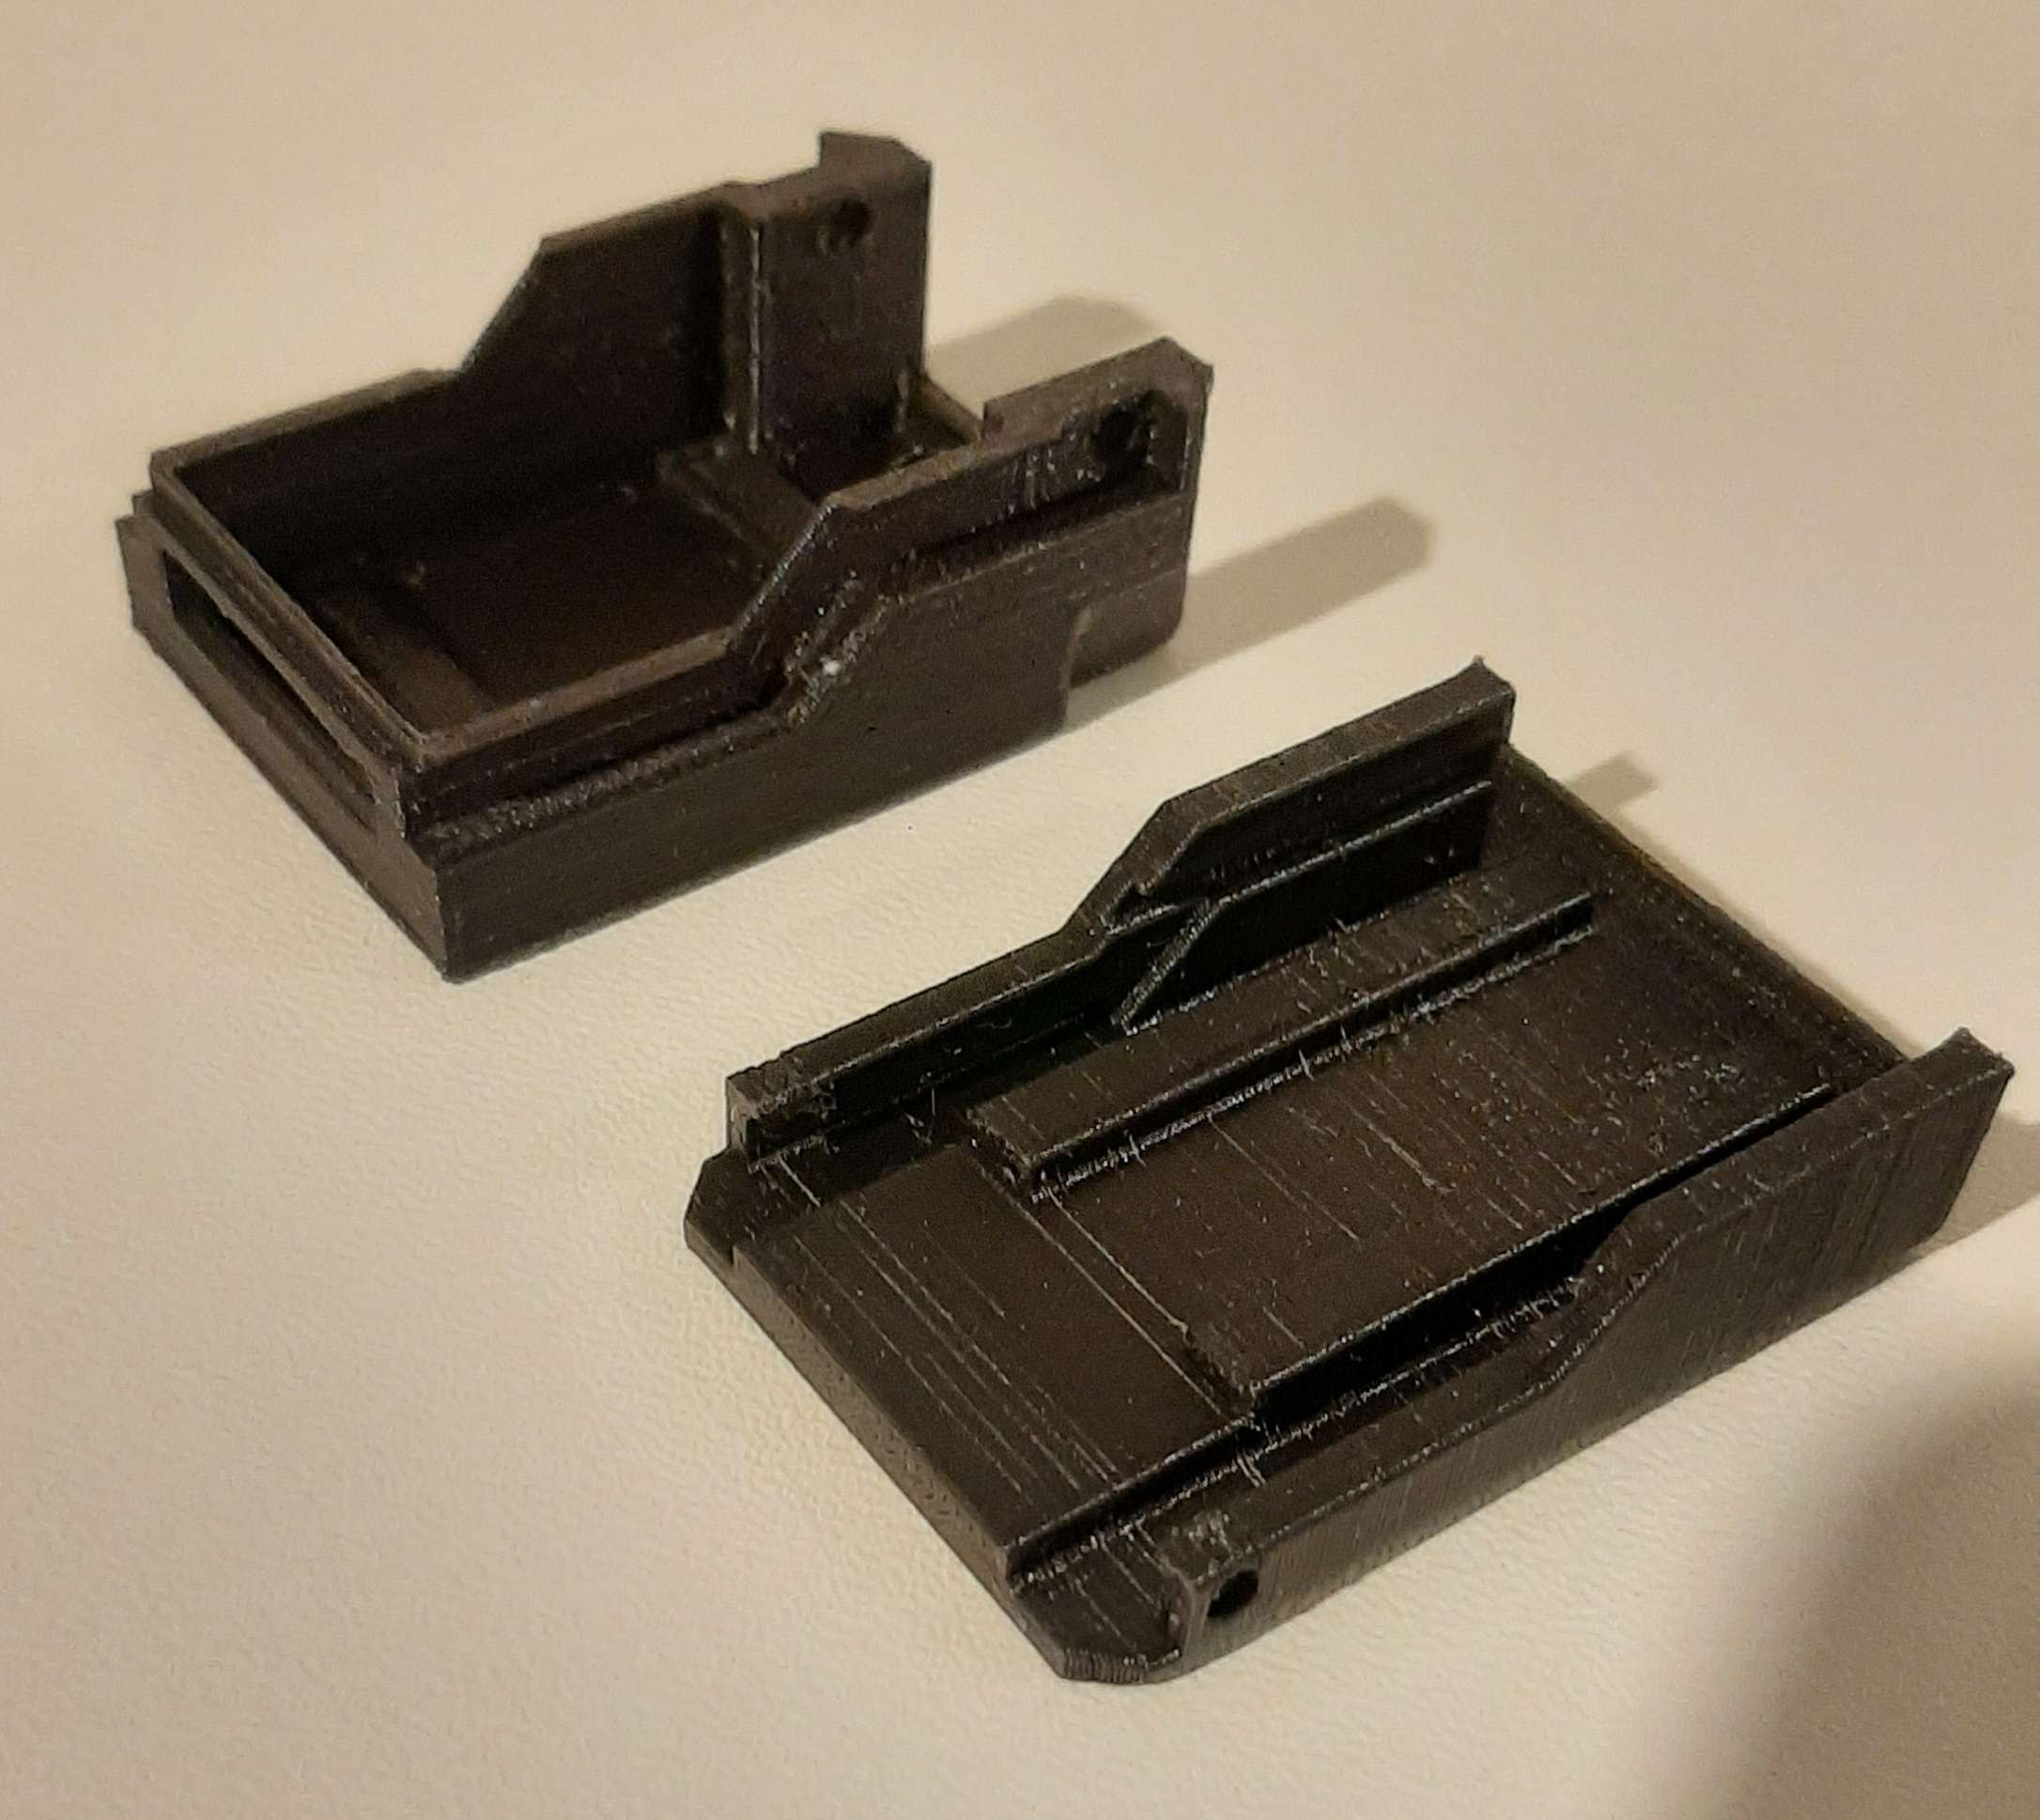
\includegraphics[scale=0.15]{obrazky/krabicka rozlozena.jpg}
    \end{center}
    \caption{Krabička čtečky čárového kódu - rozebrána}
    \label{Interakce mezi okny GUI}
\end{figure}

\begin{figure}[H]
    \begin{center}
        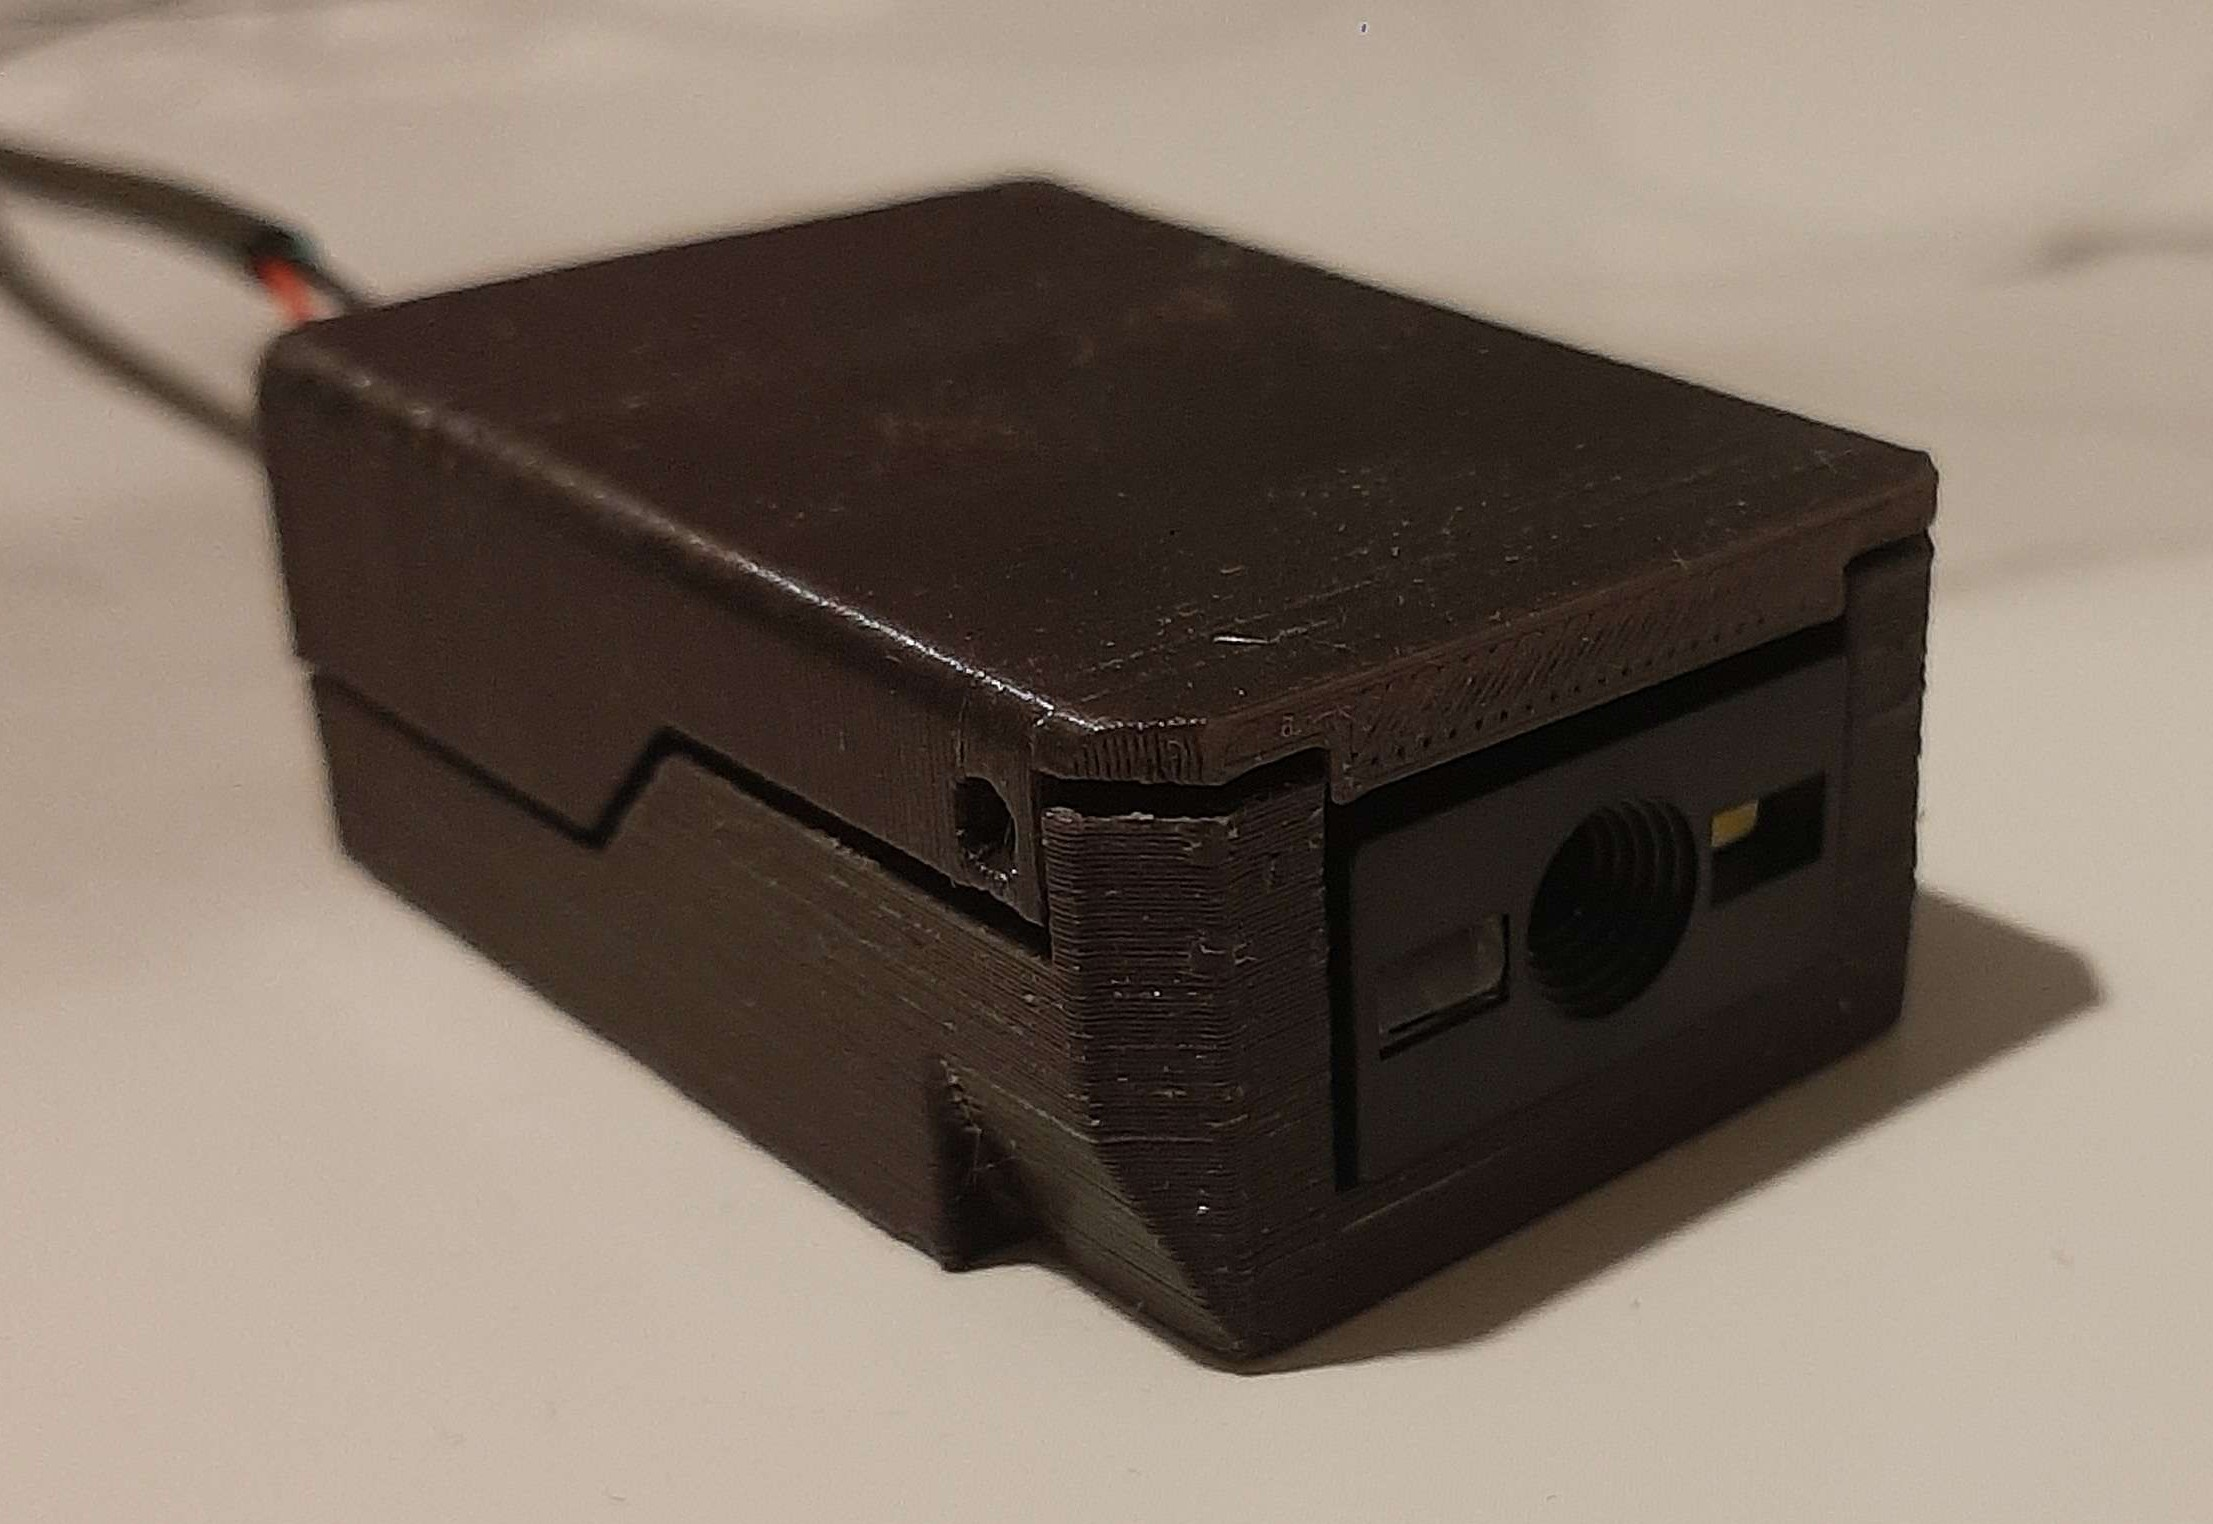
\includegraphics[scale=0.15]{obrazky/krabicka slozena.jpg}
    \end{center}
    \caption{Krabička čtečky čárového kódu - složena}
    \label{Interakce mezi okny GUI}
\end{figure}


//DODĚLAT DOKUMENTACI

\chapter{Naměřená data}

\section{Naměřené hmotnosti prázdných lahví}

\section{Tabulka naměřených objemů neotevřených lahví}

\begin{table}[h]
    \centering
    \begin{tabular}{|c|c|c|c|}
        \hline
         & \textbf{$m_{max}$ [g]} & \textbf{$m_{min}$ [g]} & \textbf{$m_{kap}$ [g]} \\ \hline \hline
        1 & 910.14 & 432.42 & 477.72 \\ \hline
        2 & 908.37 & 432.78 & 475.59 \\ \hline
        3 & 909.14 & 433.01 & 476.13 \\ \hline
        4 & 905.82 & 432.23 & 473.59 \\ \hline
        5 & 911.43 & 432.84 & 478.59 \\ \hline
        6 & 907.48 & 432.31 & 475.17 \\ \hline
        7 & 906.14 & 433.92 & 472.22 \\ \hline
        8 & 904.9 & 433.61 & 471.29 \\ \hline
        9 & 908.31 & 433.35 & 474.96 \\ \hline
        10 & 906.41 & 433.77 & 472.64 \\ \hline
        11 & 907.74 & 432.43 & 475.31 \\ \hline
        12 & 908.29 & 433.77 & 474.52 \\ \hline
        13 & 906.83 & 432.93 & 473.9 \\ \hline
        14 & 909.02 & 433.61 & 475.41 \\ \hline
        15 & 907.36 & 432.87 & 474.49 \\ \hline
    \end{tabular}
    \caption{Rozptyl hmotností plné ($m_{max}$), prázdné ($m_{min}$) láhve a jejich rozdíl ($m_{kap}$) - Amundsen vodka 0,5 l}
    \label{tab:chyba_lahve_a_plnění}
\end{table}


\section{Průběhy, výpočty a tabulky nárůstu hmotnosti z důvodu orosení}

\begin{equation}
T_{ds} = \frac{243,5 \cdot ln(\frac{V}{100} \cdot e^{\frac{17,67 \cdot T}{243,5 + T}})}{17,67 - ln(\frac{V}{100} \cdot e^{\frac{17,67 \cdot T}{243,5 + T}})}
\label{rosný bod obecne}
\end{equation}
%\caption{Rovnice rosného bodu}

\(T_{ds}\) ...Rosný bod \([\mathrm{^\circ C}]\)

\(V\) ...Relativní vlhkost vzduchu \([\mathrm{\%}]\)

\(T\) ...Teplota vzduchu \([\mathrm{^\circ C}]\)

\begin{equation}
T_{ds} = \frac{243,5 \cdot ln(\frac{50}{100} \cdot e^{\frac{17,67 \cdot 20}{243,5 + 20}})}{17,67 - ln(\frac{50}{100} \cdot e^{\frac{17,67 \cdot 20}{243,5 + 20}})} = 9,27 [^\circ C]
\label{rosný bod}
\end{equation}
%\caption{Požadavek na orosení T\_ds> 5 °C}

\bigskip

% Requires: \usepackage{graphicx}
\begin{table}[H]
    \centering
    \begin{tabular}{|c|c|c|c||c|c|c|}
    \hline
    \begin{tabular}[c]{@{}c@{}}čas \\ $[\text{min}]$\end{tabular} & 
    \begin{tabular}[c]{@{}c@{}}Božkov vaj. \\ lik. (0,5 l) [g]\end{tabular} & 
    \begin{tabular}[c]{@{}c@{}}Heffron \\ (0,7 l) [g]\end{tabular} & \begin{tabular}[c]{@{}c@{}}Nivnice \\ bor. (1 l) [g]\end{tabular} & 
    \begin{tabular}[c]{@{}c@{}}$\Delta$m \\ Božkov [g]\end{tabular} & \begin{tabular}[c]{@{}c@{}}$\Delta$m \\ Heffron [g]\end{tabular} & \begin{tabular}[c]{@{}c@{}}$\Delta$m \\ Nivnice [g]\end{tabular} \\ \hline \hline
    0  & 846.02 & 1190.02 & 1487.09 & 0.00 & 0.00 & 0.00 \\ \hline
    1  & 846.06 & 1190.03 & 1487.16 & 0.04 & 0.01 & 0.07 \\ \hline
    2  & 846.09 & 1190.05 & 1487.16 & 0.07 & 0.03 & 0.07 \\ \hline
    3  & 846.09 & 1190.09 & 1487.12 & 0.07 & 0.07 & 0.03 \\ \hline
    4  & 846.12 & 1190.09 & 1487.16 & 0.10 & 0.07 & 0.07 \\ \hline
    5  & 846.15 & 1190.12 & 1487.22 & 0.13 & 0.10 & 0.13 \\ \hline
    6  & 846.12 & 1190.22 & 1487.36 & 0.10 & 0.20 & 0.27 \\ \hline
    7  & 846.14 & 1190.21 & 1487.36 & 0.12 & 0.19 & 0.27 \\ \hline
    8  & 846.18 & 1190.22 & 1487.39 & 0.16 & 0.20 & 0.30 \\ \hline
    9  & 846.14 & 1190.25 & 1487.45 & 0.12 & 0.23 & 0.36 \\ \hline
    10 & 846.18 & 1190.31 & 1487.52 & 0.16 & 0.29 & 0.43 \\ \hline
    15 & 846.19 & 1190.32 & 1487.56 & 0.17 & 0.30 & 0.47 \\ \hline
    20 & 846.13 & 1190.35 & 1487.53 & 0.11 & 0.33 & 0.44 \\ \hline
    25 & 846.14 & 1190.31 & 1487.57 & 0.12 & 0.29 & 0.48 \\ \hline
    30 & 846.14 & 1190.37 & 1487.62 & 0.12 & 0.35 & 0.53 \\ \hline
    35 & 846.13 & 1190.38 & 1487.62 & 0.11 & 0.36 & 0.53 \\ \hline
    40 & 846.19 & 1190.47 & 1487.69 & 0.17 & 0.45 & 0.60 \\ \hline
    45 & 846.17 & 1190.41 & 1487.71 & 0.15 & 0.39 & 0.62 \\ \hline
    50 & 846.13 & 1190.46 & 1487.74 & 0.11 & 0.44 & 0.65 \\ \hline
    55 & 846.12 & 1190.39 & 1487.68 & 0.10 & 0.37 & 0.59 \\ \hline
    60 & 846.12 & 1190.30 & 1487.67 & 0.10 & 0.28 & 0.58 \\ \hline
    \end{tabular}
    %\caption{Vliv orosení na hmotnost láhve}
    \caption{Změna hmotnosti lahve vlivem orosení}
    \label{tab:measurement_data}
\end{table}

\begin{figure}[H]
    \begin{center}
        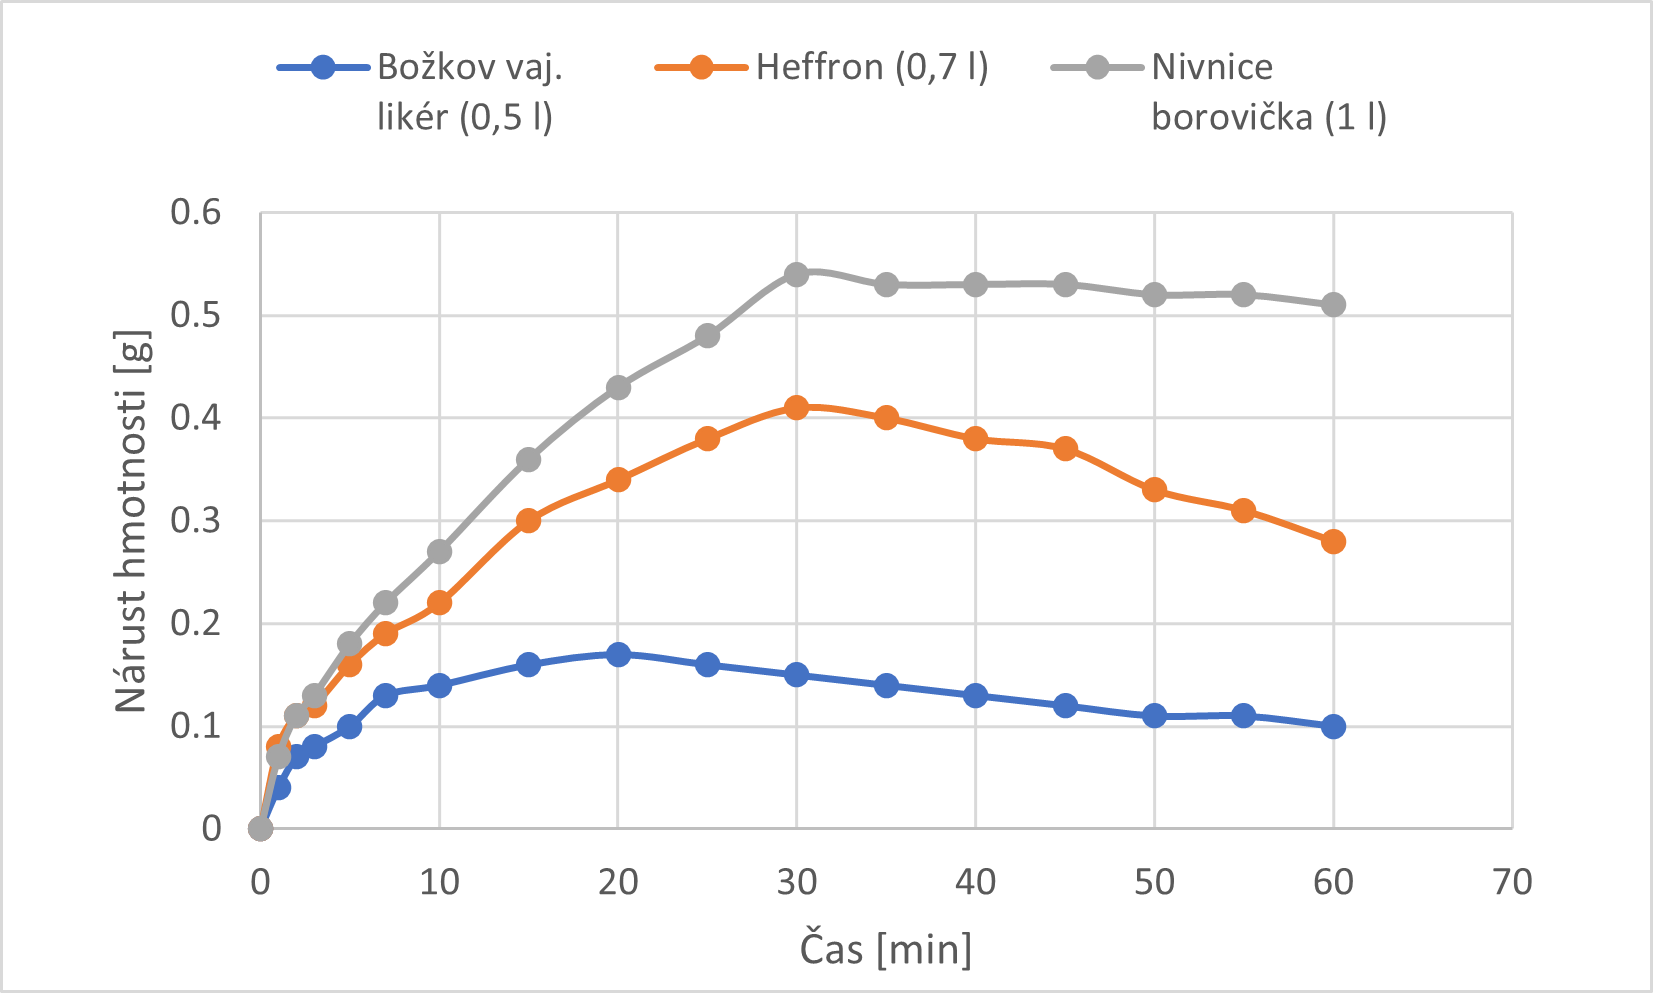
\includegraphics[scale=1.2]{obrazky/orosení.png}
    \end{center}
    \caption{Nárůst hmotnosti při orosení láhve}
\end{figure}

\chapter{Ostatní okna grafického prostředí firemwaru}

\begin{figure}[!h]
    \begin{center}
        
\includegraphics[scale=0.22]{obrazky/GUI Spuštění inventury.png}
        \includegraphics[scale=0.22]{obrazky/GUI Duplicidita.png}  
    \end{center}
    \caption{Úvodní okno firemwaru}
    \label{Úvodní okno aplikace}
\end{figure}

%\begin{figure}[H]
%    \begin{center}
%        \includegraphics[scale=0.4]{obrazky/GUI Duplicidita.png}
%    \end{center}
%    \caption{Okno informující o duplicitní evidenci produktu}
%    \label{Okno informující o duplicitní evidenci produktu}
%\end{figure}

\begin{figure}[H]
    \begin{center}
        \includegraphics[scale=0.2]{obrazky/GUI Nastavení.png}
        \includegraphics[scale=0.2]{obrazky/GUI Vymazání inventury.png}
    \end{center}
    \caption{Okno s nastavením firemwaru}
    \label{Okno s nastavením aplikace}
\end{figure}

\begin{figure}[H]
    \begin{center}
        \includegraphics[scale=0.4]{obrazky/GUI Vymazání inventury.png}
    \end{center}
    \caption{Potvrzovací okno pro vymazání aktuálně spuštěné inventury}
    \label{Potvrzovací okno pro vymazání aktuálně spuštěné inventury}
\end{figure}



\chapter{Příručka GUI}


\end{document}